% RDT2 Technical Report - Main File
% Theme: Beaver
% Compile with: pdflatex main.tex (twice for TOC)

\documentclass[aspectratio=169, 11pt]{beamer}

%==============================================================================
% THEME: BEAVER
%==============================================================================
\usetheme{default}
\usecolortheme{beaver}

% Remove navigation symbols
\setbeamertemplate{navigation symbols}{}

% Show frame numbers
\setbeamertemplate{footline}[frame number]

% Adjust fonts for readability
\setbeamerfont{frametitle}{size=\Large, series=\bfseries}
\setbeamerfont{title}{size=\LARGE, series=\bfseries}
\setbeamerfont{subtitle}{size=\large}
\setbeamerfont{block title}{size=\normalsize, series=\bfseries}

% More margin space
\setbeamersize{text margin left=10mm, text margin right=10mm}

%==============================================================================
% PACKAGES
%==============================================================================
\usepackage[utf8]{inputenc}
\usepackage[T1]{fontenc}
\usepackage{tikz}
\usepackage{pgfplots}
\usepackage{amsmath, amssymb, amsfonts}
\usepackage{bm}
\usepackage{booktabs}
\usepackage{listings}
\usepackage{xcolor}
\usepackage{hyperref}
\usepackage{graphicx}
\usepackage{multirow}
\usepackage{array}
\usepackage{mathtools}

% TikZ Libraries
\usetikzlibrary{
    shapes.geometric,
    shapes.arrows,
    arrows.meta,
    positioning,
    calc,
    fit,
    backgrounds,
    decorations.pathreplacing,
    matrix
}

\pgfplotsset{compat=1.18}

%==============================================================================
% COLORS
%==============================================================================
\definecolor{qwenblue}{RGB}{70, 130, 180}
\definecolor{rdtgreen}{RGB}{60, 179, 113}
\definecolor{vqpurple}{RGB}{147, 112, 219}
\definecolor{actionorange}{RGB}{255, 165, 0}
\definecolor{encoderblue}{RGB}{100, 149, 237}
\definecolor{decodergreen}{RGB}{144, 238, 144}
\definecolor{codebookpink}{RGB}{255, 182, 193}
\definecolor{codegreen}{RGB}{0, 128, 0}
\definecolor{codegray}{RGB}{128, 128, 128}
\definecolor{backcolor}{RGB}{248, 248, 248}

%==============================================================================
% CODE LISTINGS
%==============================================================================
\lstset{
    language=Python,
    basicstyle=\ttfamily\footnotesize,
    keywordstyle=\color{blue}\bfseries,
    commentstyle=\color{codegreen},
    stringstyle=\color{red!70!black},
    showstringspaces=false,
    breaklines=true,
    frame=single,
    backgroundcolor=\color{backcolor},
    numbers=left,
    numberstyle=\tiny\color{codegray},
    tabsize=4,
    xleftmargin=6mm,
    framexleftmargin=6mm,
    aboveskip=3mm,
    belowskip=3mm
}

%==============================================================================
% CUSTOM COMMANDS
%==============================================================================
% Math
\newcommand{\vect}[1]{\bm{#1}}
\newcommand{\mat}[1]{\mathbf{#1}}
\newcommand{\tens}[1]{\mathbf{#1}}

% Formatting
\newcommand{\dimbox}[1]{\colorbox{blue!10}{\texttt{#1}}}
\newcommand{\code}[1]{\texttt{#1}}
\newcommand{\cmark}{\textcolor{green!70!black}{\checkmark}}
\newcommand{\xmark}{\textcolor{red}{\texttimes}}

%==============================================================================
% TITLE INFO
%==============================================================================
\title{RDT2: Robotics Diffusion Transformer 2}
\subtitle{Complete Technical Deep Dive}
\author{Technical Analysis for ManiSkill Integration}
\date{January 2026}
\institute{Based on RDT2 Codebase}

%==============================================================================
% DOCUMENT
%==============================================================================
\begin{document}

% Title
\begin{frame}
    \titlepage
\end{frame}

% Table of Contents
\begin{frame}{Table of Contents}
    \tableofcontents
\end{frame}

% Include all parts
%==============================================================================
% PART 1: INTRODUCTION
%==============================================================================

\section{Introduction}

%------------------------------------------------------------------------------
\begin{frame}{What is RDT2?}
    \begin{block}{Definition}
        \textbf{RDT2} = \textbf{R}obotics \textbf{D}iffusion \textbf{T}ransformer \textbf{2}
    \end{block}

    \vspace{0.5cm}
    \textbf{Core Innovation:}
    \begin{itemize}
        \item First foundation model for \textbf{zero-shot cross-embodiment} deployment
        \item Works on \textbf{unseen robots} without fine-tuning
        \item Trained on 10,000+ hours of bimanual manipulation data
    \end{itemize}
\end{frame}

%------------------------------------------------------------------------------
\begin{frame}{Supported Tasks}
    \textbf{Open-vocabulary manipulation tasks:}

    \vspace{0.5cm}
    \begin{columns}[T]
        \begin{column}{0.5\textwidth}
            \begin{itemize}
                \item Picking objects
                \item Placing objects
                \item Pressing buttons
                \item Wiping surfaces
            \end{itemize}
        \end{column}
        \begin{column}{0.5\textwidth}
            \begin{itemize}
                \item Folding fabric
                \item Table setting
                \item Archery interception
                \item General manipulation
            \end{itemize}
        \end{column}
    \end{columns}

    \vspace{0.5cm}
    \begin{alertblock}{Reaction Time}
        Archery interception achieved $\sim$100ms reaction time (human-level)
    \end{alertblock}
\end{frame}

%------------------------------------------------------------------------------
\begin{frame}{Supported Robot Platforms}
    \textbf{Zero-shot deployment (no fine-tuning required):}

    \vspace{0.8cm}
    \begin{columns}[T]
        \begin{column}{0.45\textwidth}
            \centering
            \textbf{\large UR5e}

            \vspace{0.3cm}
            \begin{itemize}
                \item Universal Robots
                \item 6-DoF industrial arm
                \item RTDE protocol (125-500 Hz)
            \end{itemize}
        \end{column}
        \begin{column}{0.45\textwidth}
            \centering
            \textbf{\large Franka FR3}

            \vspace{0.3cm}
            \begin{itemize}
                \item Franka Emika
                \item 7-DoF research arm
                \item Torque control (1000 Hz)
            \end{itemize}
        \end{column}
    \end{columns}
\end{frame}

%------------------------------------------------------------------------------
\begin{frame}{Three Pillars of RDT2}
    \begin{enumerate}
        \item \textbf{Redesigned UMI Hardware}
              \begin{itemize}
                  \item Nylon 66 + Glass fiber (CNC machined)
                  \item HTC VIVE Tracker 3.0 for 6DoF tracking
              \end{itemize}

              \vspace{0.4cm}
        \item \textbf{Massive Diverse Dataset}
              \begin{itemize}
                  \item 10,000+ hours of manipulation video
                  \item 100+ real-world home/office environments
              \end{itemize}

              \vspace{0.4cm}
        \item \textbf{3-Stage Training Pipeline}
              \begin{itemize}
                  \item Stage 1: VQ (action tokenization)
                  \item Stage 2: FM (flow-matching)
                  \item Stage 3: Distillation (coming soon)
              \end{itemize}
    \end{enumerate}
\end{frame}

%==============================================================================
\section{Model Variants}

%------------------------------------------------------------------------------
\begin{frame}{Overview: Three Model Variants}
    \begin{table}
        \centering
        \renewcommand{\arraystretch}{1.3}
        \begin{tabular}{lccc}
            \toprule
            & \textbf{RDT2-VQ} & \textbf{RDT2-FM} & \textbf{RDT2-UltraFast} \\
            \midrule
            Stage           & 1            & 2            & 3               \\
            Output Type     & Discrete     & Continuous   & Continuous      \\
            Forward Passes  & 27           & 6            & 2               \\
            Status          & \cmark       & \cmark       & Coming Soon     \\
            \bottomrule
        \end{tabular}
    \end{table}
\end{frame}

%------------------------------------------------------------------------------
\begin{frame}{RDT2-VQ: Stage 1}
    \begin{block}{Architecture}
        Fine-tuned \textbf{Qwen2.5-VL-7B-Instruct} + RVQ Action Tokenizer
    \end{block}

    \vspace{0.5cm}
    \textbf{Input:}
    \begin{itemize}
        \item 2 wrist-camera fisheye images ($384 \times 384$ each)
        \item Language instruction (e.g., "Pick up the apple.")
    \end{itemize}

    \vspace{0.3cm}
    \textbf{Output:}
    \begin{itemize}
        \item 27 discrete action tokens (autoregressive generation)
        \item Decoded to continuous actions via VQVAE
    \end{itemize}
\end{frame}

%------------------------------------------------------------------------------
\begin{frame}{RDT2-VQ: Key Properties}
    \textbf{Inference Process:}
    \begin{itemize}
        \item 27 forward passes (one per token)
        \item Autoregressive: each token depends on previous
    \end{itemize}

    \vspace{0.5cm}
    \textbf{Strengths:}
    \begin{itemize}
        \item Superior instruction-following capability
        \item Leverages full VLM language understanding
        \item Discrete tokens = stable training
    \end{itemize}

    \vspace{0.5cm}
    \textbf{Weakness:}
    \begin{itemize}
        \item Higher latency due to 27 forward passes
        \item Discretization error from tokenization
    \end{itemize}
\end{frame}

%------------------------------------------------------------------------------
\begin{frame}{RDT2-FM: Stage 2}
    \begin{block}{Architecture}
        \textbf{Frozen} Qwen2.5-VL + 400M RDT Action Expert
    \end{block}

    \vspace{0.5cm}
    \textbf{Key Changes from VQ:}
    \begin{itemize}
        \item Replace discrete tokenizer with continuous diffusion
        \item Qwen backbone is frozen (not trained)
        \item Only RDT expert is trained
    \end{itemize}

    \vspace{0.5cm}
    \textbf{Training:}
    \begin{itemize}
        \item Flow-matching loss
        \item 5 denoising steps during inference
    \end{itemize}
\end{frame}

%------------------------------------------------------------------------------
\begin{frame}{RDT2-FM: Key Properties}
    \textbf{Inference Process:}
    \begin{itemize}
        \item 1 Qwen forward (extract KV cache)
        \item 5 RDT forwards (denoising steps)
        \item Total: 6 forward passes
    \end{itemize}

    \vspace{0.5cm}
    \textbf{Strengths:}
    \begin{itemize}
        \item No discretization error
        \item Lower latency (6 vs 27 forwards)
        \item Continuous action output
    \end{itemize}

    \vspace{0.5cm}
    \textbf{Variant:}
    \begin{itemize}
        \item \textbf{RDT2-FM-Post}: Adds UR/Franka real robot data
    \end{itemize}
\end{frame}

%------------------------------------------------------------------------------
\begin{frame}{RDT2-UltraFast: Stage 3}
    \begin{block}{Architecture}
        One-step diffusion distilled from RDT2-FM
    \end{block}

    \vspace{0.5cm}
    \textbf{Method:}
    \begin{itemize}
        \item Knowledge distillation from RDT2-FM
        \item Maps noise directly to actions in single step
    \end{itemize}

    \vspace{0.5cm}
    \textbf{Inference:}
    \begin{itemize}
        \item 1 Qwen forward + 1 RDT forward = 2 total
        \item Real-time capable ($\sim$100ms)
    \end{itemize}

    \vspace{0.5cm}
    \begin{alertblock}{Status}
        Coming Soon
    \end{alertblock}
\end{frame}

%------------------------------------------------------------------------------
\begin{frame}{Inference Latency Comparison}
    \begin{table}
        \centering
        \renewcommand{\arraystretch}{1.4}
        \begin{tabular}{lcc}
            \toprule
            \textbf{Model}     & \textbf{Forward Passes} & \textbf{Relative Speed} \\
            \midrule
            RDT2-VQ            & 27                      & 1$\times$               \\
            RDT2-FM            & 6                       & $\sim$4.5$\times$       \\
            RDT2-UltraFast     & 2                       & $\sim$13.5$\times$      \\
            \bottomrule
        \end{tabular}
    \end{table}

    \vspace{0.5cm}
    \begin{block}{Note}
        Actual latency depends on hardware and batch size
    \end{block}
\end{frame}

%------------------------------------------------------------------------------
\begin{frame}{HuggingFace Model Links}
    \textbf{Available Models:}

    \vspace{0.5cm}
    \begin{itemize}
        \item \textbf{RDT2-VQ:}

              \small\texttt{robotics-diffusion-transformer/RDT2-VQ}

              \vspace{0.3cm}
        \item \textbf{RDT2-FM:}

              \small\texttt{robotics-diffusion-transformer/RDT2-FM}

              \vspace{0.3cm}
        \item \textbf{RVQ Tokenizer:}

              \small\texttt{robotics-diffusion-transformer/RVQActionTokenizer}
    \end{itemize}
\end{frame}

%------------------------------------------------------------------------------
\begin{frame}{Hardware Requirements}
    \begin{table}
        \centering
        \renewcommand{\arraystretch}{1.3}
        \begin{tabular}{lcc}
            \toprule
            \textbf{Task}          & \textbf{VRAM}  & \textbf{Example GPU}   \\
            \midrule
            Inference              & $\sim$16 GB    & RTX 4090               \\
            Fine-tune RDT only     & $\sim$16 GB    & RTX 4090               \\
            Fine-tune LoRA         & $\geq$32 GB    & A100 40GB              \\
            Fine-tune Full         & $\geq$80 GB    & A100 80GB / H100       \\
            \bottomrule
        \end{tabular}
    \end{table}

    \vspace{0.5cm}
    \textbf{Tested OS:} Ubuntu 24.04
\end{frame}

%==============================================================================
% PART 2: UMI HARDWARE, DATA FORMAT, ACTION REPRESENTATION
%==============================================================================

\section{UMI Hardware}

%------------------------------------------------------------------------------
\begin{frame}{UMI: Universal Manipulation Interface}
    \textbf{Key Design Changes from Original UMI:}

    \vspace{0.5cm}
    \begin{table}
        \centering
        \renewcommand{\arraystretch}{1.3}
        \begin{tabular}{lll}
            \toprule
            \textbf{Component} & \textbf{Original}       & \textbf{RDT2}                \\
            \midrule
            Material           & 3D Printed              & Nylon 66 + Glass Fiber       \\
            Fabrication        & FDM Printing            & CNC Machining                \\
            Tracking           & SLAM                    & HTC VIVE Tracker 3.0         \\
            Tracking Type      & Visual                  & Infrared Positioning         \\
            \bottomrule
        \end{tabular}
    \end{table}
\end{frame}

%------------------------------------------------------------------------------
\begin{frame}{Why VIVE Tracker?}
    \textbf{Problem with SLAM:}
    \begin{itemize}
        \item Unreliable in texture-less environments
        \item Fails on reflective surfaces
        \item Drift over time
    \end{itemize}

    \vspace{0.5cm}
    \textbf{VIVE Tracker 3.0 Benefits:}
    \begin{itemize}
        \item Robust 6DoF pose estimation
        \item Works in any lighting condition
        \item Sub-millimeter accuracy
        \item No drift
    \end{itemize}
\end{frame}

%------------------------------------------------------------------------------
\begin{frame}{UMI Device Components}
    Each UMI device contains:

    \vspace{0.5cm}
    \begin{enumerate}
        \item \textbf{Fisheye Camera}
              \begin{itemize}
                  \item Resolution: $384 \times 384$ RGB
                  \item Wrist-mounted ego-centric view
              \end{itemize}

              \vspace{0.3cm}
        \item \textbf{HTC VIVE Tracker 3.0}
              \begin{itemize}
                  \item Position: $(x, y, z)$ in meters
                  \item Rotation: quaternion $(w, x, y, z)$
              \end{itemize}

              \vspace{0.3cm}
        \item \textbf{Gripper}
              \begin{itemize}
                  \item Width range: $[0, 0.088]$ meters
                  \item $0$ = closed, $0.088$ = fully open
              \end{itemize}
    \end{enumerate}
\end{frame}

%------------------------------------------------------------------------------
\begin{frame}{Data Collection Statistics}
    \begin{table}
        \centering
        \renewcommand{\arraystretch}{1.4}
        \begin{tabular}{lr}
            \toprule
            \textbf{Metric}                   & \textbf{Value}         \\
            \midrule
            UMI Systems Manufactured          & $\sim$100              \\
            Collection Environments           & 100+ homes/offices     \\
            Total Video Hours                 & 10,000+                \\
            Cost vs Teleoperation             & $\sim$1/10             \\
            Speed vs Traditional              & 5$\times$ faster       \\
            \bottomrule
        \end{tabular}
    \end{table}
\end{frame}

%------------------------------------------------------------------------------
\begin{frame}{Excluded Tasks}
    \textbf{Tasks NOT covered in UMI data:}

    \vspace{0.5cm}
    \begin{itemize}
        \item Water contact tasks
        \item Heat contact tasks
        \item Five-finger dexterity
        \item Large consumable tasks
    \end{itemize}

    \vspace{0.5cm}
    \begin{block}{Implication}
        Zero-shot performance on these tasks is not guaranteed
    \end{block}
\end{frame}

%==============================================================================
\section{Data Format}

%------------------------------------------------------------------------------
\begin{frame}{WebDataset TAR Format}
    Training data stored in \textbf{WebDataset} format (TAR files):

    \vspace{0.5cm}
    \texttt{shard-XXXXXX.tar} contains:

    \vspace{0.3cm}
    \begin{table}
        \centering
        \renewcommand{\arraystretch}{1.3}
        \begin{tabular}{lll}
            \toprule
            \textbf{File}             & \textbf{Content}      & \textbf{Shape}         \\
            \midrule
            \texttt{N.image.jpg}      & Binocular RGB         & $(H, W, 3)$            \\
            \texttt{N.action.npy}     & Relative actions      & $(24, 20)$             \\
            \texttt{N.action\_token.npy} & VQ tokens          & $(27,)$                \\
            \texttt{N.meta.json}      & Metadata              & JSON                   \\
            \bottomrule
        \end{tabular}
    \end{table}
\end{frame}

%------------------------------------------------------------------------------
\begin{frame}{Image Data Format}
    \textbf{Binocular Image:}

    \vspace{0.3cm}
    \begin{itemize}
        \item Left camera: $384 \times 384 \times 3$
        \item Right camera: $384 \times 384 \times 3$
        \item Concatenated horizontally: $384 \times 768 \times 3$
    \end{itemize}

    \vspace{0.5cm}
    \textbf{Format Details:}
    \begin{itemize}
        \item Data type: \texttt{np.uint8}
        \item Color space: RGB
        \item Compression: JPEG
        \item Value range: $[0, 255]$
    \end{itemize}
\end{frame}

%------------------------------------------------------------------------------
\begin{frame}{Image Concatenation}
    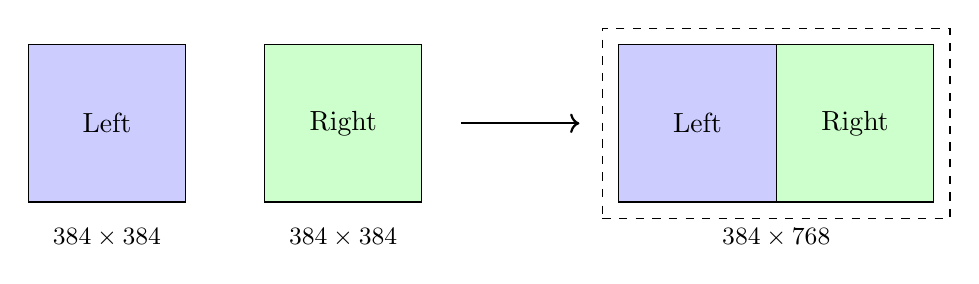
\begin{tikzpicture}
        % Left camera
        \node[draw, fill=blue!20, minimum width=2cm, minimum height=2cm] (left) at (0, 0) {Left};
        \node[below=0.2cm of left] {\small $384 \times 384$};

        % Right camera
        \node[draw, fill=green!20, minimum width=2cm, minimum height=2cm] (right) at (3, 0) {Right};
        \node[below=0.2cm of right] {\small $384 \times 384$};

        % Arrow
        \draw[->, thick] (4.5, 0) -- (6, 0);

        % Combined
        \node[draw, fill=blue!20, minimum width=2cm, minimum height=2cm] (cleft) at (7.5, 0) {Left};
        \node[draw, fill=green!20, minimum width=2cm, minimum height=2cm] (cright) at (9.5, 0) {Right};
        \node[below=0.2cm of cright, xshift=-1cm] {\small $384 \times 768$};

        % Fit box
        \node[draw, dashed, fit=(cleft)(cright), inner sep=2mm] {};
    \end{tikzpicture}
\end{frame}

%------------------------------------------------------------------------------
\begin{frame}{Action Data Format}
    \textbf{Action Tensor:}
    \begin{equation}
        \tens{A} \in \mathbb{R}^{B \times T \times D}
    \end{equation}

    where:
    \begin{itemize}
        \item $B$ = Batch size
        \item $T = 24$ (timesteps)
        \item $D = 20$ (action dimensions for bimanual)
    \end{itemize}

    \vspace{0.5cm}
    \textbf{Properties:}
    \begin{itemize}
        \item Data type: \texttt{float32}
        \item Values: relative deltas between frames
        \item Duration: 0.8 seconds @ 30 Hz
    \end{itemize}
\end{frame}

%------------------------------------------------------------------------------
\begin{frame}{Action Token Format}
    \textbf{Token Tensor:}
    \begin{equation}
        \vect{t} \in \mathbb{Z}^{B \times 27}
    \end{equation}

    \vspace{0.3cm}
    \textbf{Properties:}
    \begin{itemize}
        \item Data type: \texttt{int16}
        \item Value range: $[0, 1023]$
        \item Codebook size: 1024
        \item Total tokens: 27 per action chunk
    \end{itemize}

    \vspace{0.5cm}
    \textbf{Token Distribution:}
    \begin{itemize}
        \item Position: 18 tokens
        \item Rotation: 9 tokens
        \item Gripper: 3 tokens (actual: varies)
    \end{itemize}
\end{frame}

%------------------------------------------------------------------------------
\begin{frame}[fragile]{Metadata JSON}
    \textbf{Contents of \texttt{N.meta.json}:}

    \vspace{0.5cm}
\begin{lstlisting}
{
    "sub_task_instruction_key": "/path/to/instruction"
}
\end{lstlisting}

    \vspace{0.5cm}
    \textbf{Purpose:}
    \begin{itemize}
        \item Links sample to instruction file
        \item Contains task-specific metadata
        \item Used for instruction lookup during training
    \end{itemize}
\end{frame}

%==============================================================================
\section{Action Representation}

%------------------------------------------------------------------------------
\begin{frame}{20-D Bimanual Action Structure}
    \textbf{Total: 20 dimensions = 10 per arm $\times$ 2 arms}

    \vspace{0.5cm}
    \begin{equation}
        \vect{a} = [\underbrace{a_0, \ldots, a_9}_{\text{Right arm}}, \underbrace{a_{10}, \ldots, a_{19}}_{\text{Left arm}}]
    \end{equation}
\end{frame}

%------------------------------------------------------------------------------
\begin{frame}{Action Index Mapping}
    \begin{table}
        \centering
        \renewcommand{\arraystretch}{1.3}
        \begin{tabular}{clcc}
            \toprule
            \textbf{Indices}            & \textbf{Description}     & \textbf{Dim} & \textbf{Arm}  \\
            \midrule
            $[0, 1, 2]$                 & Position $(x, y, z)$     & 3            & Right         \\
            $[3, 4, 5, 6, 7, 8]$        & Rotation (6D)            & 6            & Right         \\
            $[9]$                       & Gripper width            & 1            & Right         \\
            \midrule
            $[10, 11, 12]$              & Position $(x, y, z)$     & 3            & Left          \\
            $[13, 14, 15, 16, 17, 18]$  & Rotation (6D)            & 6            & Left          \\
            $[19]$                      & Gripper width            & 1            & Left          \\
            \bottomrule
        \end{tabular}
    \end{table}
\end{frame}

%------------------------------------------------------------------------------
\begin{frame}{Per-Arm Action Structure (10-D)}
    \textbf{Each robot arm uses 10 dimensions:}

    \vspace{0.5cm}
    \begin{equation}
        \vect{a}_{\text{arm}} = \begin{bmatrix}
            \underbrace{p_x, p_y, p_z}_{\text{Position (3)}} &
            \underbrace{r_1, r_2, r_3, r_4, r_5, r_6}_{\text{Rotation (6)}} &
            \underbrace{g}_{\text{Gripper (1)}}
        \end{bmatrix}
    \end{equation}

    \vspace{0.5cm}
    \textbf{Units:}
    \begin{itemize}
        \item Position: meters (relative delta)
        \item Rotation: 6D representation (unitless)
        \item Gripper: meters ($[0, 0.088]$)
    \end{itemize}
\end{frame}

%------------------------------------------------------------------------------
\begin{frame}{Why 6D Rotation?}
    \textbf{Problems with other representations:}

    \vspace{0.3cm}
    \begin{itemize}
        \item \textbf{Euler angles:}
              \begin{itemize}
                  \item Gimbal lock at certain orientations
                  \item Discontinuous
              \end{itemize}

        \item \textbf{Quaternions:}
              \begin{itemize}
                  \item Double cover: $q$ and $-q$ are same rotation
                  \item Discontinuity at antipodal points
              \end{itemize}

        \item \textbf{Axis-angle:}
              \begin{itemize}
                  \item Discontinuity at $\theta = 0$
              \end{itemize}
    \end{itemize}
\end{frame}

%------------------------------------------------------------------------------
\begin{frame}{6D Rotation: Advantages}
    \textbf{Benefits of 6D representation (Zhou et al., 2019):}

    \vspace{0.5cm}
    \begin{itemize}
        \item \textbf{Continuous:} No discontinuities
        \item \textbf{No singularities:} Works for all rotations
        \item \textbf{Learnable:} Easy for neural networks
        \item \textbf{Geodesic loss:} Enables proper rotation loss
    \end{itemize}

    \vspace{0.5cm}
    \begin{block}{Key Insight}
        First two columns of rotation matrix are sufficient!
    \end{block}
\end{frame}

%------------------------------------------------------------------------------
\begin{frame}{6D to Rotation Matrix: Theory}
    \textbf{Given 6D vector:}
    \begin{equation}
        \vect{r} = [a_1, a_2, a_3, a_4, a_5, a_6]^\top
    \end{equation}

    \textbf{Step 1: Extract vectors}
    \begin{equation}
        \vect{a}_1 = [a_1, a_2, a_3]^\top, \quad \vect{a}_2 = [a_4, a_5, a_6]^\top
    \end{equation}
\end{frame}

%------------------------------------------------------------------------------
\begin{frame}{6D to Rotation Matrix: Gram-Schmidt}
    \textbf{Step 2: Orthonormalize (Gram-Schmidt)}

    \vspace{0.3cm}
    \begin{align}
        \vect{b}_1 &= \frac{\vect{a}_1}{\|\vect{a}_1\|_2} \\[0.3cm]
        \vect{b}_2 &= \frac{\vect{a}_2 - (\vect{b}_1^\top \vect{a}_2)\vect{b}_1}{\|\vect{a}_2 - (\vect{b}_1^\top \vect{a}_2)\vect{b}_1\|_2} \\[0.3cm]
        \vect{b}_3 &= \vect{b}_1 \times \vect{b}_2
    \end{align}

    \textbf{Step 3: Construct matrix}
    \begin{equation}
        \mat{R} = [\vect{b}_1 \mid \vect{b}_2 \mid \vect{b}_3] \in SO(3)
    \end{equation}
\end{frame}

%------------------------------------------------------------------------------
\begin{frame}[fragile]{6D to Matrix: Code}
\begin{lstlisting}
def rot6d_to_mat(rot6d):
    """Convert 6D rotation to 3x3 matrix.
    Input: rot6d [..., 6]
    Output: mat [..., 3, 3]
    """
    a1 = rot6d[..., :3]
    a2 = rot6d[..., 3:]

    # Normalize first vector
    b1 = F.normalize(a1, dim=-1)

    # Orthogonalize second vector
    dot = (b1 * a2).sum(dim=-1, keepdim=True)
    b2 = F.normalize(a2 - dot * b1, dim=-1)

    # Cross product
    b3 = torch.cross(b1, b2, dim=-1)

    return torch.stack([b1, b2, b3], dim=-1)
\end{lstlisting}
\end{frame}

%------------------------------------------------------------------------------
\begin{frame}{Geodesic Distance for Rotations}
    \textbf{Definition:} Angular distance on $SO(3)$ manifold

    \vspace{0.5cm}
    \begin{equation}
        d_{\text{geo}}(\mat{R}_1, \mat{R}_2) = \arccos\left(\frac{\text{tr}(\mat{R}_1^\top \mat{R}_2) - 1}{2}\right)
    \end{equation}

    \vspace{0.5cm}
    \textbf{Properties:}
    \begin{itemize}
        \item Range: $[0, \pi]$ radians
        \item Metric on $SO(3)$
        \item Measures rotation angle between matrices
    \end{itemize}
\end{frame}

%------------------------------------------------------------------------------
\begin{frame}{Geodesic Loss Function}
    \textbf{For training rotation prediction:}

    \vspace{0.5cm}
    \begin{equation}
        \mathcal{L}_{\text{geo}} = \frac{1}{n}\sum_{i=1}^{n} \arccos\left(\frac{\text{tr}(\mat{R}_{\text{pred},i}^\top \mat{R}_{\text{gt},i}) - 1}{2}\right)
    \end{equation}

    \vspace{0.5cm}
    \textbf{Normalized version:}
    \begin{equation}
        \mathcal{L}_{\text{geo,norm}} = \frac{\mathcal{L}_{\text{geo}}}{\pi} \in [0, 1]
    \end{equation}
\end{frame}

%------------------------------------------------------------------------------
\begin{frame}[fragile]{Geodesic Loss: Code}
\begin{lstlisting}
def geodesic_loss(R_pred, R_gt, eps=1e-7):
    """Compute geodesic loss.
    Input: R_pred, R_gt [..., 3, 3]
    Output: loss (scalar)
    """
    # R_err = R_pred^T @ R_gt
    R_err = torch.matmul(
        R_pred.transpose(-1, -2), R_gt
    )

    # trace = sum of diagonal
    trace = R_err.diagonal(dim1=-2, dim2=-1).sum(-1)

    # cos(theta) = (trace - 1) / 2
    cos_theta = (trace - 1) / 2
    cos_theta = torch.clamp(cos_theta, -1+eps, 1-eps)

    # loss = arccos(cos_theta)
    return torch.acos(cos_theta).mean()
\end{lstlisting}
\end{frame}

%------------------------------------------------------------------------------
\begin{frame}{Gripper Width Details}
    \textbf{Range:} $g \in [0, 0.088]$ meters

    \vspace{0.5cm}
    \begin{itemize}
        \item $g = 0$: Fully closed
        \item $g = 0.088$: Fully open (UMI gripper max)
    \end{itemize}

    \vspace{0.5cm}
    \begin{alertblock}{Critical: Rescaling Required}
        For real robot deployment:
        \begin{equation}
            g_{\text{robot}} = \frac{g_{\text{model}}}{0.088} \times g_{\text{max,robot}}
        \end{equation}
        Example: If robot max is 0.10m:
        \begin{equation}
            g_{\text{robot}} = \frac{g_{\text{model}}}{0.088} \times 0.10
        \end{equation}
    \end{alertblock}
\end{frame}

%------------------------------------------------------------------------------
\begin{frame}{Action Chunk: Temporal Structure}
    \textbf{One action chunk = 24 frames @ 30 Hz}

    \vspace{0.5cm}
    \begin{equation}
        \text{Duration} = \frac{24 \text{ frames}}{30 \text{ Hz}} = 0.8 \text{ seconds}
    \end{equation}

    \vspace{0.5cm}
    \textbf{Tensor shape:}
    \begin{equation}
        \tens{A} \in \mathbb{R}^{24 \times 20}
    \end{equation}

    \vspace{0.3cm}
    \begin{itemize}
        \item Row $i$: action at timestep $i$ (20 dimensions)
        \item Column $j$: dimension $j$ across all timesteps
    \end{itemize}
\end{frame}

%------------------------------------------------------------------------------
\begin{frame}{Action Chunk: Visual Timeline}
    \begin{center}
    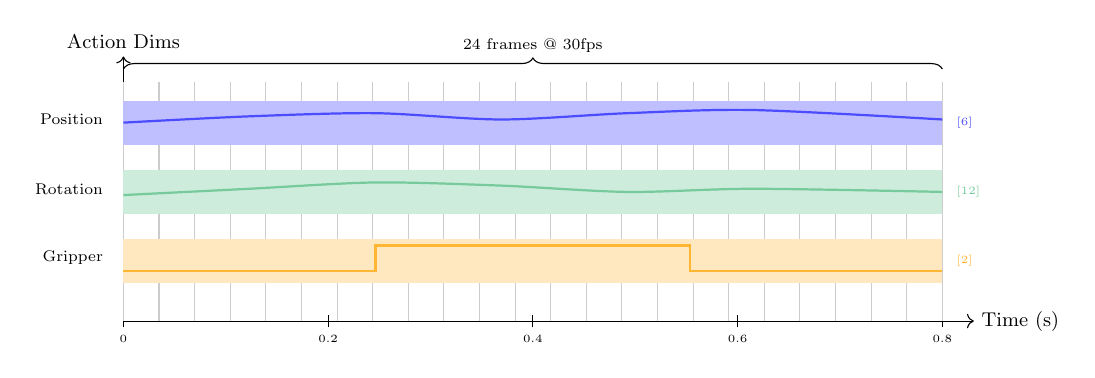
\begin{tikzpicture}[scale=0.8, transform shape]
        % Time axis
        \draw[->] (0,0) -- (13.5,0) node[right, font=\small] {Time (s)};
        \draw[->] (0,0) -- (0,4.2) node[above, font=\small] {Action Dims};

        % Time markers
        \foreach \x/\t in {0/0, 3.25/0.2, 6.5/0.4, 9.75/0.6, 13/0.8} {
            \draw (\x,-0.1) -- (\x,0.1);
            \node[below, font=\tiny] at (\x,-0.1) {\t};
        }

        % Frame markers (24 frames)
        \foreach \i in {0,...,23} {
            \pgfmathsetmacro{\x}{\i * 13 / 23}
            \draw[gray!40] (\x,0) -- (\x,3.8);
        }

        % Position component
        \begin{scope}[shift={(0,2.8)}]
            \node[left, font=\scriptsize] at (-0.2,0.4) {Position};
            \fill[blue!25] (0,0) rectangle (13,0.7);
            \draw[blue!70, thick] plot[smooth] coordinates {
                (0,0.35) (2,0.45) (4,0.5) (6,0.4) (8,0.5) (10,0.55) (13,0.4)
            };
            \node[right, font=\tiny, blue!70] at (13.1,0.35) {[6]};
        \end{scope}

        % Rotation component
        \begin{scope}[shift={(0,1.7)}]
            \node[left, font=\scriptsize] at (-0.2,0.4) {Rotation};
            \fill[rdtgreen!25] (0,0) rectangle (13,0.7);
            \draw[rdtgreen!70, thick] plot[smooth] coordinates {
                (0,0.3) (2,0.4) (4,0.5) (6,0.45) (8,0.35) (10,0.4) (13,0.35)
            };
            \node[right, font=\tiny, rdtgreen!70] at (13.1,0.35) {[12]};
        \end{scope}

        % Gripper component
        \begin{scope}[shift={(0,0.6)}]
            \node[left, font=\scriptsize] at (-0.2,0.4) {Gripper};
            \fill[actionorange!25] (0,0) rectangle (13,0.7);
            \draw[actionorange!80, thick] (0,0.2) -- (4,0.2) -- (4,0.6) -- (9,0.6) -- (9,0.2) -- (13,0.2);
            \node[right, font=\tiny, actionorange!80] at (13.1,0.35) {[2]};
        \end{scope}

        % Brace annotation
        \draw[decorate, decoration={brace, amplitude=4pt}] (0,4) -- (13,4)
            node[midway, above=4pt, font=\scriptsize] {24 frames @ 30fps};
    \end{tikzpicture}
    \end{center}

    \vspace{0.2cm}
    \textbf{Total:} 20 dimensions (bimanual: 10 per arm)
\end{frame}

%------------------------------------------------------------------------------
\begin{frame}{Control Frequency}
    \textbf{Model outputs 24 actions per inference}

    \vspace{0.5cm}
    \textbf{Execution strategies:}
    \begin{enumerate}
        \item \textbf{Execute all 24:}
              \begin{itemize}
                  \item Run at 30 Hz
                  \item New inference every 0.8s
              \end{itemize}

              \vspace{0.3cm}
        \item \textbf{Action chunking:}
              \begin{itemize}
                  \item Execute only first $k$ actions
                  \item Re-predict more frequently
                  \item Better reactivity
              \end{itemize}
    \end{enumerate}
\end{frame}

% TODO: Create these files
% %==============================================================================
% PART 3: VQVAE ACTION TOKENIZER
%==============================================================================

\section{VQVAE Action Tokenizer}

%------------------------------------------------------------------------------
\begin{frame}{VQVAE Overview}
    \begin{block}{Purpose}
        Convert \textbf{continuous actions} to \textbf{discrete tokens} for autoregressive VLA
    \end{block}

    \vspace{0.5cm}
    \textbf{Why Tokenize Actions?}
    \begin{itemize}
        \item Leverage VLM's discrete token prediction capability
        \item Enable autoregressive generation (like text)
        \item Unified interface with language tokens
    \end{itemize}

    \vspace{0.5cm}
    \begin{alertblock}{Key Innovation}
        RDT2 uses \textbf{Residual VQ} with component separation:
        \begin{itemize}
            \item Only 27 tokens for 0.8s action chunk
            \item 3--8$\times$ shorter than prior methods
        \end{itemize}
    \end{alertblock}
\end{frame}

%------------------------------------------------------------------------------
\begin{frame}{Vector Quantization: Core Concept}
    \begin{block}{Definition}
        Map continuous encoder output $\vect{z}_e$ to nearest codebook entry $\vect{w}_k$
    \end{block}

    \vspace{0.3cm}
    \textbf{Codebook:} $\mathcal{W} = \{\vect{w}_1, \vect{w}_2, \ldots, \vect{w}_Z\}$, where $Z = 1024$

    \vspace{0.5cm}
    \textbf{Quantization:}
    \[
        k^* = \argmin_{k \in \{1, \ldots, Z\}} \| \bar{\vect{z}}_e - \bar{\vect{w}}_k \|^2
    \]

    where $\bar{\vect{z}} = \frac{\vect{z}}{\|\vect{z}\|}$ (L2 normalization)

    \vspace{0.5cm}
    \textbf{Quantized output:}
    \[
        \vect{z}_q = \vect{w}_{k^*}
    \]
\end{frame}

%------------------------------------------------------------------------------
\begin{frame}{Distance Calculation}
    \textbf{Euclidean distance with L2-normalized vectors:}

    \vspace{0.3cm}
    \[
        d(\bar{\vect{z}}_e, \bar{\vect{w}}_k) = \|\bar{\vect{z}}_e\|^2 - 2 \bar{\vect{z}}_e^T \bar{\vect{w}}_k + \|\bar{\vect{w}}_k\|^2
    \]

    \vspace{0.3cm}
    Since $\|\bar{\vect{z}}\| = 1$ after normalization:
    \[
        d(\bar{\vect{z}}_e, \bar{\vect{w}}_k) = 2 - 2 \bar{\vect{z}}_e^T \bar{\vect{w}}_k = 2(1 - \cos\theta)
    \]

    \vspace{0.5cm}
    \begin{alertblock}{Cosine Similarity}
        L2 normalization converts Euclidean distance to \textbf{cosine similarity}:
        \[
            \argmin_k d(\bar{\vect{z}}_e, \bar{\vect{w}}_k) = \argmax_k \cos(\bar{\vect{z}}_e, \bar{\vect{w}}_k)
        \]
        This improves training stability (ViT-VQGAN)
    \end{alertblock}
\end{frame}

%------------------------------------------------------------------------------
\begin{frame}{VQ Loss Functions}
    \textbf{Three loss components:}

    \vspace{0.5cm}
    \textbf{1. Commitment Loss} (encoder $\rightarrow$ codebook):
    \[
        \mathcal{L}_{\text{commit}} = \| \vect{z}_e - \text{sg}[\vect{z}_q] \|^2
    \]

    \vspace{0.3cm}
    \textbf{2. Codebook Loss} (codebook $\rightarrow$ encoder):
    \[
        \mathcal{L}_{\text{cb}} = \| \vect{z}_q - \text{sg}[\vect{z}_e] \|^2
    \]

    \vspace{0.3cm}
    \textbf{3. Total VQ Loss:}
    \[
        \boxed{\mathcal{L}_{\text{VQ}} = \beta \cdot \mathcal{L}_{\text{commit}} + \gamma \cdot \mathcal{L}_{\text{cb}}}
    \]

    \vspace{0.3cm}
    where $\text{sg}[\cdot]$ = stop-gradient operator

    \vspace{0.3cm}
    \begin{block}{Default Values}
        $\beta = 0.25$ (commitment\_cost), $\gamma = 0$ (codebook\_cost)
    \end{block}
\end{frame}

%------------------------------------------------------------------------------
\begin{frame}{Straight-Through Estimator}
    \begin{block}{Problem}
        Quantization is \textbf{non-differentiable} (argmin operation)
    \end{block}

    \vspace{0.5cm}
    \textbf{Solution: Straight-Through Gradient}

    \vspace{0.3cm}
    \textbf{Forward pass:}
    \[
        \vect{z}_q = \text{Quantize}(\vect{z}_e) = \vect{w}_{k^*}
    \]

    \vspace{0.3cm}
    \textbf{Backward pass:}
    \[
        \frac{\partial \mathcal{L}}{\partial \vect{z}_e} = \frac{\partial \mathcal{L}}{\partial \vect{z}_q}
    \]

    \vspace{0.3cm}
    \textbf{Implementation:}
    \[
        \boxed{\vect{z}_q = \vect{z}_e + \text{sg}[\vect{z}_q - \vect{z}_e]}
    \]

    \vspace{0.3cm}
    \begin{alertblock}{Interpretation}
        Forward: output is $\vect{z}_q$ (quantized) \\
        Backward: gradient flows directly to $\vect{z}_e$ (copies gradient)
    \end{alertblock}
\end{frame}

%------------------------------------------------------------------------------
\begin{frame}{EMA Codebook Update}
    \begin{block}{Why EMA?}
        More stable than gradient-based updates for codebook learning
    \end{block}

    \vspace{0.3cm}
    \textbf{Track cluster statistics:}
    \begin{itemize}
        \item $N_i^{(t)}$: count of vectors assigned to codebook entry $i$
        \item $\vect{m}_i^{(t)}$: sum of encoder outputs assigned to entry $i$
    \end{itemize}

    \vspace{0.3cm}
    \textbf{EMA Update Rules:}
    \begin{align*}
        N_i^{(t)} &= \gamma \cdot N_i^{(t-1)} + (1 - \gamma) \cdot n_i \\
        \vect{m}_i^{(t)} &= \gamma \cdot \vect{m}_i^{(t-1)} + (1 - \gamma) \sum_{j: \text{idx}(j)=i} \vect{z}_e^{(j)}
    \end{align*}

    \vspace{0.3cm}
    \textbf{Codebook Update (with Laplace smoothing):}
    \[
        \boxed{\vect{w}_i = \frac{\vect{m}_i}{\tilde{N}_i}}, \quad \tilde{N}_i = \frac{(N_i + \epsilon)}{(N + Z \epsilon)} \cdot N
    \]

    Default: $\gamma = 0.99$, $\epsilon = 10^{-5}$
\end{frame}

%------------------------------------------------------------------------------
\begin{frame}{Factorized Codes}
    \begin{block}{Motivation}
        Improve codebook utilization by separating dimensions
    \end{block}

    \vspace{0.5cm}
    \textbf{Architecture:}
    \begin{center}
    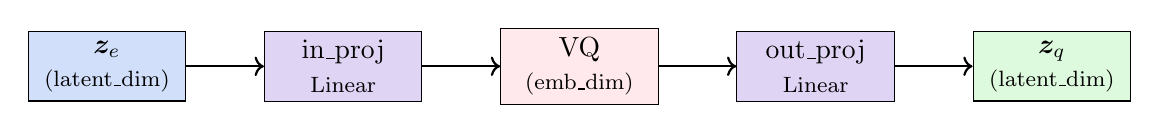
\begin{tikzpicture}[
        box/.style={rectangle, draw, minimum width=2cm, minimum height=0.8cm, align=center},
        arrow/.style={->, thick}
    ]
        \node[box, fill=encoderblue!30] (ze) at (0,0) {$\vect{z}_e$\\{\footnotesize (latent\_dim)}};
        \node[box, fill=vqpurple!30] (proj_in) at (3,0) {in\_proj\\{\footnotesize Linear}};
        \node[box, fill=codebookpink!30] (vq) at (6,0) {VQ\\{\footnotesize (emb\_dim)}};
        \node[box, fill=vqpurple!30] (proj_out) at (9,0) {out\_proj\\{\footnotesize Linear}};
        \node[box, fill=decodergreen!30] (zq) at (12,0) {$\vect{z}_q$\\{\footnotesize (latent\_dim)}};

        \draw[arrow] (ze) -- (proj_in);
        \draw[arrow] (proj_in) -- (vq);
        \draw[arrow] (vq) -- (proj_out);
        \draw[arrow] (proj_out) -- (zq);
    \end{tikzpicture}
    \end{center}

    \vspace{0.5cm}
    \textbf{Dimension Flow:}
    \[
        \underbrace{64}_{\text{latent}} \xrightarrow{\text{in\_proj}} \underbrace{256}_{\text{embedding}} \xrightarrow{\text{VQ}} \underbrace{256}_{\text{embedding}} \xrightarrow{\text{out\_proj}} \underbrace{64}_{\text{latent}}
    \]

    \vspace{0.3cm}
    \begin{alertblock}{Benefit}
        Codebook lookup happens in lower-dimensional space, improving usage
    \end{alertblock}
\end{frame}

%------------------------------------------------------------------------------
\begin{frame}{Codebook Restart}
    \begin{block}{Problem: Dead Entries}
        Some codebook entries are never selected $\rightarrow$ wasted capacity
    \end{block}

    \vspace{0.5cm}
    \textbf{Tracking Dead Entries:}
    \begin{itemize}
        \item Maintain \code{entry\_hits} buffer of size $[P, Z]$
        \item $P = 64$ (restart period), $Z = 1024$ (codebook size)
        \item Track which entries were selected each iteration
    \end{itemize}

    \vspace{0.3cm}
    \textbf{Restart Condition (every $P$ iterations):}
    \[
        \text{dead\_entries} = \{ i : \sum_{t=1}^{P} \text{hits}_{t,i} = 0 \}
    \]

    \vspace{0.3cm}
    \textbf{Restart Process:}
    \begin{enumerate}
        \item Gather encoder outputs from all GPUs
        \item Randomly select from current batch
        \item Re-initialize dead entries with selected vectors
    \end{enumerate}
\end{frame}

%------------------------------------------------------------------------------
\begin{frame}{Residual VQ Algorithm}
    \begin{block}{Key Idea}
        Quantize residuals iteratively for better reconstruction
    \end{block}

    \vspace{0.3cm}
    \begin{columns}[T]
        \begin{column}{0.55\textwidth}
            \textbf{Algorithm:}
            \begin{algorithmic}[1]
                \State \textbf{Input:} $\vect{z}$, codebooks $\{VQ_1, \ldots, VQ_N\}$
                \State $\vect{r} \leftarrow \vect{z}$ \Comment{residual}
                \State $\vect{z}_q \leftarrow \vect{0}$
                \For{$i = 1$ to $N$}
                    \State $\vect{z}_{q,i}, idx_i \leftarrow VQ_i(\vect{r})$
                    \State $\vect{z}_q \leftarrow \vect{z}_q + \vect{z}_{q,i}$
                    \State $\vect{r} \leftarrow \vect{r} - \vect{z}_{q,i}$
                \EndFor
                \State \textbf{Return:} $\vect{z}_q$, $[idx_1, \ldots, idx_N]$
            \end{algorithmic}
        \end{column}
        \begin{column}{0.4\textwidth}
            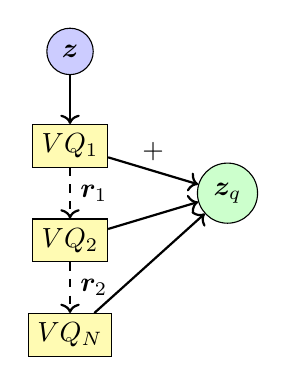
\begin{tikzpicture}[scale=0.8]
                \node[draw, circle, fill=blue!20] (z) at (0,3) {$\vect{z}$};
                \node[draw, rectangle, fill=yellow!30] (vq1) at (0,1.5) {$VQ_1$};
                \node[draw, rectangle, fill=yellow!30] (vq2) at (0,0) {$VQ_2$};
                \node[draw, rectangle, fill=yellow!30] (vq3) at (0,-1.5) {$VQ_N$};
                \node[draw, circle, fill=green!20] (zq) at (2.5,0.75) {$\vect{z}_q$};

                \draw[->, thick] (z) -- (vq1);
                \draw[->, thick, dashed] (vq1) -- node[right] {$\vect{r}_1$} (vq2);
                \draw[->, thick, dashed] (vq2) -- node[right] {$\vect{r}_2$} (vq3);
                \draw[->, thick] (vq1) -- node[above] {$+$} (zq);
                \draw[->, thick] (vq2) -- (zq);
                \draw[->, thick] (vq3) -- (zq);
            \end{tikzpicture}
        \end{column}
    \end{columns}

    \vspace{0.3cm}
    \textbf{Decoding:}
    \[
        \vect{z}_q = \sum_{i=1}^{N} VQ_i.\text{decode}(idx_i)
    \]
\end{frame}

%------------------------------------------------------------------------------
\begin{frame}{RVQ: Mathematical Formulation}
    \textbf{Encoding (per timestep):}
    \begin{align*}
        \vect{r}^{(0)} &= \vect{z} \\
        \vect{z}_{q}^{(i)}, idx^{(i)} &= VQ_i(\vect{r}^{(i-1)}) \\
        \vect{r}^{(i)} &= \vect{r}^{(i-1)} - \vect{z}_{q}^{(i)}
    \end{align*}

    \vspace{0.3cm}
    \textbf{Final Output:}
    \[
        \boxed{\vect{z}_q = \sum_{i=1}^{N} \vect{z}_{q}^{(i)}}
    \]

    \vspace{0.3cm}
    \textbf{Loss Aggregation:}
    \[
        \mathcal{L}_{\text{RVQ}} = \sum_{i=1}^{N} \mathcal{L}_{\text{VQ}}^{(i)}
    \]

    \vspace{0.3cm}
    \begin{block}{Token Sequence}
        For $N$ codebooks: output is $N$ tokens per timestep \\
        Each token $\in \{0, 1, \ldots, Z-1\}$ where $Z = 1024$
    \end{block}
\end{frame}

%------------------------------------------------------------------------------
\begin{frame}{Encoder CNN Architecture}
    \textbf{8$\times$ Temporal Compression:} $[B, D, 24] \rightarrow [B, C, 3]$

    \vspace{0.3cm}
    \begin{center}
    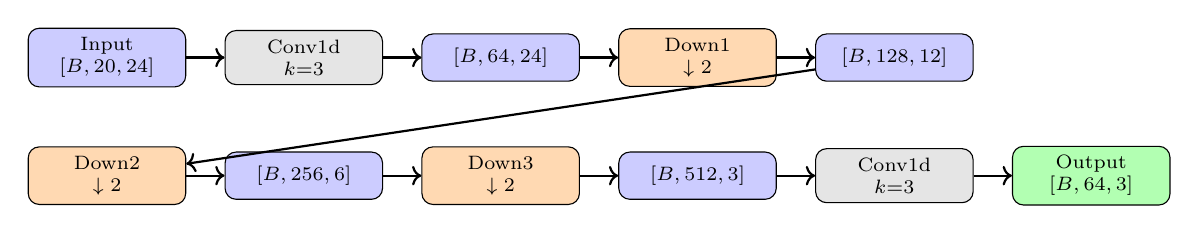
\begin{tikzpicture}[
        block/.style={rectangle, draw, rounded corners, minimum width=2cm, minimum height=0.6cm, align=center, font=\scriptsize},
        arrow/.style={->, thick}
    ]
        % Input
        \node[block, fill=blue!20] (input) at (0,0) {Input\\$[B, 20, 24]$};

        % Conv in
        \node[block, fill=gray!20] (conv_in) at (2.5,0) {Conv1d\\$k{=}3$};
        \node[block, fill=blue!20] (c1) at (5,0) {$[B, 64, 24]$};

        % Down block 1
        \node[block, fill=orange!30] (down1) at (7.5,0) {Down1\\$\downarrow 2$};
        \node[block, fill=blue!20] (c2) at (10,0) {$[B, 128, 12]$};

        % Down block 2
        \node[block, fill=orange!30] (down2) at (0,-1.5) {Down2\\$\downarrow 2$};
        \node[block, fill=blue!20] (c3) at (2.5,-1.5) {$[B, 256, 6]$};

        % Down block 3
        \node[block, fill=orange!30] (down3) at (5,-1.5) {Down3\\$\downarrow 2$};
        \node[block, fill=blue!20] (c4) at (7.5,-1.5) {$[B, 512, 3]$};

        % Conv out
        \node[block, fill=gray!20] (conv_out) at (10,-1.5) {Conv1d\\$k{=}3$};
        \node[block, fill=green!30] (output) at (12.5,-1.5) {Output\\$[B, 64, 3]$};

        \draw[arrow] (input) -- (conv_in);
        \draw[arrow] (conv_in) -- (c1);
        \draw[arrow] (c1) -- (down1);
        \draw[arrow] (down1) -- (c2);
        \draw[arrow] (c2) -- (down2);
        \draw[arrow] (down2) -- (c3);
        \draw[arrow] (c3) -- (down3);
        \draw[arrow] (down3) -- (c4);
        \draw[arrow] (c4) -- (conv_out);
        \draw[arrow] (conv_out) -- (output);
    \end{tikzpicture}
    \end{center}

    \vspace{0.3cm}
    \textbf{Down Block Structure:}
    \[
        \text{ConvBlock}(ch \rightarrow 2ch) \rightarrow \text{Downsample2x} \rightarrow \text{ConvBlock}
    \]

    \textbf{ConvBlock:} GroupNorm $\rightarrow$ SiLU $\rightarrow$ Conv1d $\rightarrow$ Dropout
\end{frame}

%------------------------------------------------------------------------------
\begin{frame}{Decoder CNN Architecture}
    \textbf{8$\times$ Temporal Upsampling:} $[B, C, 3] \rightarrow [B, D, 24]$

    \vspace{0.3cm}
    \begin{center}
    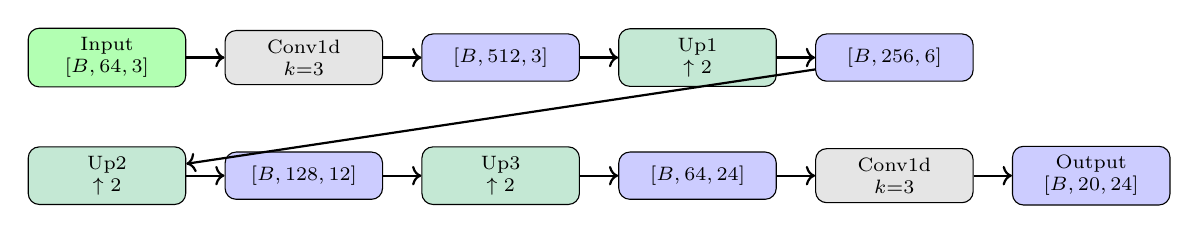
\begin{tikzpicture}[
        block/.style={rectangle, draw, rounded corners, minimum width=2cm, minimum height=0.6cm, align=center, font=\scriptsize},
        arrow/.style={->, thick}
    ]
        % Input
        \node[block, fill=green!30] (input) at (0,0) {Input\\$[B, 64, 3]$};

        % Conv in
        \node[block, fill=gray!20] (conv_in) at (2.5,0) {Conv1d\\$k{=}3$};
        \node[block, fill=blue!20] (c1) at (5,0) {$[B, 512, 3]$};

        % Up block 1
        \node[block, fill=rdtgreen!30] (up1) at (7.5,0) {Up1\\$\uparrow 2$};
        \node[block, fill=blue!20] (c2) at (10,0) {$[B, 256, 6]$};

        % Up block 2
        \node[block, fill=rdtgreen!30] (up2) at (0,-1.5) {Up2\\$\uparrow 2$};
        \node[block, fill=blue!20] (c3) at (2.5,-1.5) {$[B, 128, 12]$};

        % Up block 3
        \node[block, fill=rdtgreen!30] (up3) at (5,-1.5) {Up3\\$\uparrow 2$};
        \node[block, fill=blue!20] (c4) at (7.5,-1.5) {$[B, 64, 24]$};

        % Conv out
        \node[block, fill=gray!20] (conv_out) at (10,-1.5) {Conv1d\\$k{=}3$};
        \node[block, fill=blue!20] (output) at (12.5,-1.5) {Output\\$[B, 20, 24]$};

        \draw[arrow] (input) -- (conv_in);
        \draw[arrow] (conv_in) -- (c1);
        \draw[arrow] (c1) -- (up1);
        \draw[arrow] (up1) -- (c2);
        \draw[arrow] (c2) -- (up2);
        \draw[arrow] (up2) -- (c3);
        \draw[arrow] (c3) -- (up3);
        \draw[arrow] (up3) -- (c4);
        \draw[arrow] (c4) -- (conv_out);
        \draw[arrow] (conv_out) -- (output);
    \end{tikzpicture}
    \end{center}

    \vspace{0.3cm}
    \textbf{Up Block Structure:}
    \[
        \text{ConvBlock} \rightarrow \text{Upsample2x\_TF} \rightarrow \text{ConvBlock}(ch \rightarrow ch/2)
    \]

    \textbf{Upsample2x\_TF:} Transposed convolution with $k=4$, $s=2$, $p=1$
\end{frame}

%------------------------------------------------------------------------------
\begin{frame}{MultiVQVAE: Component Separation}
    \begin{block}{Key Innovation}
        Separate tokenizers for \textbf{position}, \textbf{rotation}, and \textbf{gripper}
    \end{block}

    \vspace{0.3cm}
    \begin{center}
    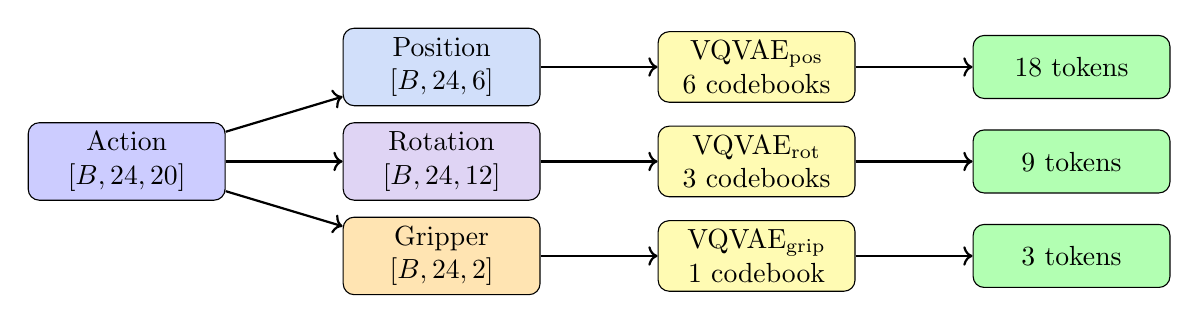
\begin{tikzpicture}[
        box/.style={rectangle, draw, rounded corners, minimum width=2.5cm, minimum height=0.8cm, align=center},
        arrow/.style={->, thick}
    ]
        % Input
        \node[box, fill=blue!20] (input) at (0,0) {Action\\$[B, 24, 20]$};

        % Split
        \node[box, fill=encoderblue!30] (pos) at (4,1.2) {Position\\$[B, 24, 6]$};
        \node[box, fill=vqpurple!30] (rot) at (4,0) {Rotation\\$[B, 24, 12]$};
        \node[box, fill=actionorange!30] (grip) at (4,-1.2) {Gripper\\$[B, 24, 2]$};

        % VQVAEs
        \node[box, fill=yellow!30] (vq_pos) at (8,1.2) {VQVAE$_\text{pos}$\\6 codebooks};
        \node[box, fill=yellow!30] (vq_rot) at (8,0) {VQVAE$_\text{rot}$\\3 codebooks};
        \node[box, fill=yellow!30] (vq_grip) at (8,-1.2) {VQVAE$_\text{grip}$\\1 codebook};

        % Tokens
        \node[box, fill=green!30] (tok_pos) at (12,1.2) {18 tokens};
        \node[box, fill=green!30] (tok_rot) at (12,0) {9 tokens};
        \node[box, fill=green!30] (tok_grip) at (12,-1.2) {3 tokens};

        \draw[arrow] (input) -- (pos);
        \draw[arrow] (input) -- (rot);
        \draw[arrow] (input) -- (grip);
        \draw[arrow] (pos) -- (vq_pos);
        \draw[arrow] (rot) -- (vq_rot);
        \draw[arrow] (grip) -- (vq_grip);
        \draw[arrow] (vq_pos) -- (tok_pos);
        \draw[arrow] (vq_rot) -- (tok_rot);
        \draw[arrow] (vq_grip) -- (tok_grip);
    \end{tikzpicture}
    \end{center}

    \vspace{0.3cm}
    \textbf{Total Tokens:} $18 + 9 + 3 = 30 \rightarrow 27$ (after optimization)
\end{frame}

%------------------------------------------------------------------------------
\begin{frame}{Token Distribution}
    \begin{table}
        \centering
        \renewcommand{\arraystretch}{1.4}
        \begin{tabular}{lcccc}
            \toprule
            \textbf{Component} & \textbf{Dim} & \textbf{Codebooks} & \textbf{Timesteps} & \textbf{Tokens} \\
            \midrule
            Position & 6 & 6 & 3 & $6 \times 3 = 18$ \\
            Rotation & 12 & 3 & 3 & $3 \times 3 = 9$ \\
            Gripper & 2 & 1 & 3 & $1 \times 3 = 3$ \\
            \midrule
            \textbf{Total} & 20 & 10 & -- & \textbf{30 $\rightarrow$ 27} \\
            \bottomrule
        \end{tabular}
    \end{table}

    \vspace{0.5cm}
    \textbf{Compression Analysis:}
    \begin{itemize}
        \item Input: $24 \times 20 = 480$ float values
        \item Output: 27 discrete tokens
        \item Compression ratio: $\sim$18$\times$
        \item Each token: $\log_2(1024) = 10$ bits
    \end{itemize}
\end{frame}

%------------------------------------------------------------------------------
\begin{frame}{Action Dimension Mapping}
    \textbf{20-dim Bimanual Action $\rightarrow$ 3 Components:}

    \vspace{0.5cm}
    \begin{table}
        \centering
        \renewcommand{\arraystretch}{1.3}
        \begin{tabular}{lcc}
            \toprule
            \textbf{Component} & \textbf{Right Arm Indices} & \textbf{Left Arm Indices} \\
            \midrule
            Position (6D) & [0, 1, 2] & [10, 11, 12] \\
            Rotation (12D) & [3, 4, 5, 6, 7, 8] & [13, 14, 15, 16, 17, 18] \\
            Gripper (2D) & [9] & [19] \\
            \bottomrule
        \end{tabular}
    \end{table}

    \vspace{0.5cm}
    \textbf{Code Implementation:}
    \begin{itemize}
        \item \code{select\_act\_dim(x, 'pos')}: Extract [0:3, 10:13]
        \item \code{select\_act\_dim(x, 'rot')}: Extract [3:9, 13:19]
        \item \code{select\_act\_dim(x, 'grip')}: Extract [9, 19]
    \end{itemize}

    \vspace{0.3cm}
    \textbf{Reconstruction:}
    \begin{itemize}
        \item \code{apply\_act\_dim(x, y, 'pos')}: Insert at [0:3, 10:13]
        \item Same for rotation and gripper
    \end{itemize}
\end{frame}

%------------------------------------------------------------------------------
\begin{frame}{Token Conversion: VLA $\leftrightarrow$ VAE}
    \begin{block}{Problem}
        VLA vocabulary tokens $\neq$ VAE codebook indices
    \end{block}

    \vspace{0.5cm}
    \textbf{VLA to VAE Conversion:}
    \[
        \boxed{t_{\text{vae}} = V_{\text{vocab}} - (t_{\text{vla}} + 1)}
    \]

    \vspace{0.3cm}
    \textbf{VAE to VLA Conversion:}
    \[
        \boxed{t_{\text{vla}} = V_{\text{vocab}} - t_{\text{vae}} - 1}
    \]

    \vspace{0.3cm}
    where $V_{\text{vocab}} = 152064$ (Qwen2.5-VL vocabulary size)

    \vspace{0.5cm}
    \textbf{Clamping for Valid Range:}
    \[
        t_{\text{vae}} = \text{clamp}(t_{\text{vae}}, 0, Z-1)
    \]
    where $Z = 1024$ (codebook size)

    \begin{alertblock}{Note}
        Invalid tokens (out of range) indicate generation errors
    \end{alertblock}
\end{frame}

%------------------------------------------------------------------------------
\begin{frame}{Complete VQVAE Pipeline}
    \begin{center}
    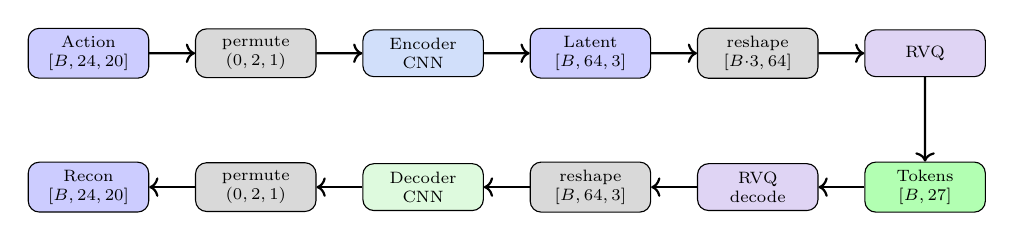
\begin{tikzpicture}[
        box/.style={rectangle, draw, rounded corners, minimum width=1.8cm, minimum height=0.7cm, align=center, font=\scriptsize},
        arrow/.style={->, thick},
        scale=0.85, transform shape
    ]
        % Encoding path
        \node[box, fill=blue!20] (input) at (0,2) {Action\\$[B,24,20]$};
        \node[box, fill=gray!30] (perm1) at (2.5,2) {permute\\$(0,2,1)$};
        \node[box, fill=encoderblue!30] (enc) at (5,2) {Encoder\\CNN};
        \node[box, fill=blue!20] (latent) at (7.5,2) {Latent\\$[B,64,3]$};
        \node[box, fill=gray!30] (reshape1) at (10,2) {reshape\\$[B{\cdot}3,64]$};
        \node[box, fill=vqpurple!30] (rvq) at (12.5,2) {RVQ};

        % Token output
        \node[box, fill=green!30] (tokens) at (12.5,0) {Tokens\\$[B,27]$};

        % Decoding path
        \node[box, fill=vqpurple!30] (rvq_dec) at (10,0) {RVQ\\decode};
        \node[box, fill=gray!30] (reshape2) at (7.5,0) {reshape\\$[B,64,3]$};
        \node[box, fill=decodergreen!30] (dec) at (5,0) {Decoder\\CNN};
        \node[box, fill=gray!30] (perm2) at (2.5,0) {permute\\$(0,2,1)$};
        \node[box, fill=blue!20] (output) at (0,0) {Recon\\$[B,24,20]$};

        % Arrows
        \draw[arrow] (input) -- (perm1);
        \draw[arrow] (perm1) -- (enc);
        \draw[arrow] (enc) -- (latent);
        \draw[arrow] (latent) -- (reshape1);
        \draw[arrow] (reshape1) -- (rvq);
        \draw[arrow] (rvq) -- (tokens);
        \draw[arrow] (tokens) -- (rvq_dec);
        \draw[arrow] (rvq_dec) -- (reshape2);
        \draw[arrow] (reshape2) -- (dec);
        \draw[arrow] (dec) -- (perm2);
        \draw[arrow] (perm2) -- (output);
    \end{tikzpicture}
    \end{center}

    \vspace{0.5cm}
    \textbf{Key Dimension Transformations:}
    \begin{align*}
        [B, 24, 20] &\xrightarrow{\text{permute}} [B, 20, 24] \xrightarrow{\text{Encoder}} [B, 64, 3] \\
        &\xrightarrow{\text{reshape}} [B \cdot 3, 64] \xrightarrow{\text{RVQ}} [B \cdot 3, N] \\
        &\xrightarrow{\text{flatten}} [B, 3 \cdot N] = [B, 27]
    \end{align*}
\end{frame}

%------------------------------------------------------------------------------
\begin{frame}{Codebook Parameters}
    \begin{table}
        \centering
        \renewcommand{\arraystretch}{1.4}
        \begin{tabular}{lccccc}
            \toprule
            \textbf{Parameter} & \textbf{Position} & \textbf{Rotation} & \textbf{Gripper} \\
            \midrule
            Input dim ($D$) & 6 & 12 & 2 \\
            Latent dim ($C$) & 64 & 64 & 64 \\
            Embedding dim ($E$) & 256 & 256 & 256 \\
            Codebook size ($Z$) & 1024 & 1024 & 1024 \\
            Num codebooks ($N$) & 6 & 3 & 1 \\
            \midrule
            Tokens per timestep & 6 & 3 & 1 \\
            Timesteps & 3 & 3 & 3 \\
            \textbf{Total tokens} & \textbf{18} & \textbf{9} & \textbf{3} \\
            \bottomrule
        \end{tabular}
    \end{table}

    \vspace{0.3cm}
    \begin{block}{Default Hyperparameters}
        \begin{itemize}
            \item EMA decay: $\gamma = 0.99$
            \item Commitment cost: $\beta = 0.25$
            \item Codebook restart interval: 64 iterations
        \end{itemize}
    \end{block}
\end{frame}

%------------------------------------------------------------------------------
\begin{frame}{VQVAE Loss Components}
    \textbf{Total Training Loss:}
    \[
        \mathcal{L}_{\text{total}} = \mathcal{L}_{\text{recon}} + \mathcal{L}_{\text{VQ}}
    \]

    \vspace{0.3cm}
    \textbf{1. Reconstruction Loss (per component):}
    \begin{itemize}
        \item Position: MSE loss
              \[ \mathcal{L}_{\text{pos}} = \|\hat{\vect{p}} - \vect{p}\|^2 \]
        \item Rotation: Geodesic loss (6D representation)
              \[ \mathcal{L}_{\text{rot}} = \arccos\left(\frac{\text{tr}(\mat{R}_{\text{pred}}^T \mat{R}_{\text{gt}}) - 1}{2}\right) \]
        \item Gripper: MSE loss
              \[ \mathcal{L}_{\text{grip}} = \|\hat{g} - g\|^2 \]
    \end{itemize}

    \vspace{0.3cm}
    \textbf{2. VQ Loss:}
    \[
        \mathcal{L}_{\text{VQ}} = \sum_{c \in \{\text{pos}, \text{rot}, \text{grip}\}} \mathcal{L}_{\text{VQ}}^{(c)}
    \]
\end{frame}

%------------------------------------------------------------------------------
\begin{frame}{HuggingFace Model}
    \textbf{Model Location:}

    \vspace{0.3cm}
    \code{robotics-diffusion-transformer/RVQActionTokenizer}

    \vspace{0.5cm}
    \textbf{Loading in Code:}
    \begin{lstlisting}[language=Python, basicstyle=\ttfamily\small]
from vqvae.models.multivqvae import MultiVQVAE

vae = MultiVQVAE.from_pretrained(
    "robotics-diffusion-transformer/RVQActionTokenizer"
)
vae = vae.to("cuda").float()
    \end{lstlisting}

    \vspace{0.5cm}
    \textbf{Key Attributes:}
    \begin{itemize}
        \item \code{vae.pos\_id\_len} = 18
        \item \code{vae.rot\_id\_len} = 9
        \item \code{vae.grip\_id\_len} = 3
        \item \code{vae.num\_embeddings} = 1024
    \end{itemize}
\end{frame}

%------------------------------------------------------------------------------
\begin{frame}{Encode/Decode Example}
    \textbf{Encoding Actions to Tokens:}
    \begin{lstlisting}[language=Python, basicstyle=\ttfamily\small]
# actions: [B, 24, 20] - normalized action chunk
with torch.no_grad():
    tokens = vae.encode(actions)  # [B, 27]
    \end{lstlisting}

    \vspace{0.5cm}
    \textbf{Decoding Tokens to Actions:}
    \begin{lstlisting}[language=Python, basicstyle=\ttfamily\small]
# tokens: [B, 27] - from VLA generation
with torch.no_grad():
    actions_recon = vae.decode(tokens)  # [B, 24, 20]
    \end{lstlisting}

    \vspace{0.5cm}
    \textbf{Component-wise Decoding:}
    \begin{lstlisting}[language=Python, basicstyle=\ttfamily\small]
result = vae.decode(tokens, return_dict=True)
# result['pos']: [B, 24, 6]
# result['rot']: [B, 24, 12]
# result['grip']: [B, 24, 2]
    \end{lstlisting}
\end{frame}

%------------------------------------------------------------------------------
\begin{frame}{VQVAE Summary}
    \begin{columns}[T]
        \begin{column}{0.5\textwidth}
            \textbf{Key Techniques:}
            \begin{itemize}
                \item L2 normalization (cosine similarity)
                \item Straight-through estimator
                \item EMA codebook updates
                \item Codebook restart for dead entries
                \item Residual quantization
                \item Component separation
            \end{itemize}
        \end{column}
        \begin{column}{0.5\textwidth}
            \textbf{Output Specification:}
            \begin{itemize}
                \item 27 discrete tokens
                \item Each token $\in [0, 1023]$
                \item Position: 18 tokens
                \item Rotation: 9 tokens
                \item Gripper: 3 tokens
            \end{itemize}
        \end{column}
    \end{columns}

    \vspace{0.5cm}
    \begin{alertblock}{Comparison with Prior Methods}
        \begin{itemize}
            \item ACT: 256 tokens per chunk
            \item RT-2: 256 tokens per step
            \item \textbf{RDT2: 27 tokens per chunk (0.8s)}
            \item $\mathbf{3\text{--}8\times}$ \textbf{shorter token sequences}
        \end{itemize}
    \end{alertblock}
\end{frame}


% %==============================================================================
% PART 4: RDT2-VQ ARCHITECTURE
%==============================================================================

\section{RDT2-VQ Architecture}

%------------------------------------------------------------------------------
\begin{frame}{RDT2-VQ Overview}
    \begin{block}{Definition}
        \textbf{RDT2-VQ} = Vision-Language-Action model with VQ action tokenization
    \end{block}

    \vspace{0.5cm}
    \textbf{Core Architecture:}
    \begin{itemize}
        \item \textbf{Backbone:} Qwen2.5-VL-7B-Instruct (fine-tuned)
        \item \textbf{Action Output:} Discrete tokens via VQVAE
        \item \textbf{Generation:} Autoregressive (27 tokens)
    \end{itemize}

    \vspace{0.5cm}
    \begin{alertblock}{Key Characteristic}
        \textbf{27 forward passes} per action chunk (one per token)
    \end{alertblock}
\end{frame}

%------------------------------------------------------------------------------
\begin{frame}{Qwen2.5-VL-7B-Instruct}
    \begin{columns}[T]
        \begin{column}{0.55\textwidth}
            \begin{block}{Base Model}
                Alibaba's VLM with instruction following
            \end{block}

            \vspace{0.2cm}
            \textbf{Model Specifications:}
            \begin{table}
                \centering
                \footnotesize
                \renewcommand{\arraystretch}{1.2}
                \begin{tabular}{ll}
                    \toprule
                    \textbf{Parameter} & \textbf{Value} \\
                    \midrule
                    Parameters & 7B \\
                    Hidden size & 3584 \\
                    Num layers & 28 \\
                    Vocabulary size & 152,064 \\
                    \bottomrule
                \end{tabular}
            \end{table}
        \end{column}
        \begin{column}{0.45\textwidth}
            \textbf{Key Features:}
            \begin{itemize}
                \item Multi-image support
                \item Flash Attention 2
                \item Instruction-tuned
                \item ViT vision encoder
            \end{itemize}
        \end{column}
    \end{columns}
\end{frame}

%------------------------------------------------------------------------------
\begin{frame}{RDT2-VQ Architecture Diagram}
    \begin{center}
    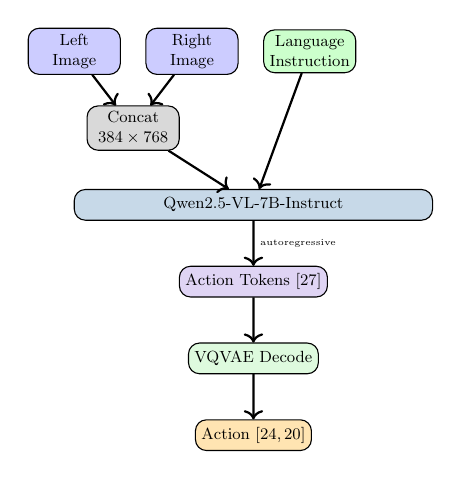
\begin{tikzpicture}[
        box/.style={rectangle, draw, rounded corners, minimum width=1.8cm, minimum height=0.6cm, align=center, font=\small},
        arrow/.style={->, thick},
        scale=0.65, transform shape
    ]
        % Input
        \node[box, fill=blue!20] (img_l) at (0,2.5) {Left\\Image};
        \node[box, fill=blue!20] (img_r) at (2.3,2.5) {Right\\Image};
        \node[box, fill=green!20] (text) at (4.6,2.5) {Language\\Instruction};

        % Concatenate
        \node[box, fill=gray!30] (concat) at (1.15,1) {Concat\\$384 \times 768$};

        % Qwen processor
        \node[box, fill=qwenblue!30, minimum width=7cm] (qwen) at (3.5,-0.5) {Qwen2.5-VL-7B-Instruct};

        % Output
        \node[box, fill=vqpurple!30] (tokens) at (3.5,-2) {Action Tokens $[27]$};

        % VAE decode
        \node[box, fill=decodergreen!30] (vae) at (3.5,-3.5) {VQVAE Decode};

        % Final output
        \node[box, fill=actionorange!30] (action) at (3.5,-5) {Action $[24, 20]$};

        % Arrows
        \draw[arrow] (img_l) -- (concat);
        \draw[arrow] (img_r) -- (concat);
        \draw[arrow] (concat) -- (qwen);
        \draw[arrow] (text) -- (qwen);
        \draw[arrow] (qwen) -- node[right, font=\tiny] {autoregressive} (tokens);
        \draw[arrow] (tokens) -- (vae);
        \draw[arrow] (vae) -- (action);
    \end{tikzpicture}
    \end{center}
\end{frame}

%------------------------------------------------------------------------------
\begin{frame}{Image Input Processing (1/2)}
    \textbf{Binocular Fisheye Images:}

    \vspace{0.3cm}
    \begin{center}
    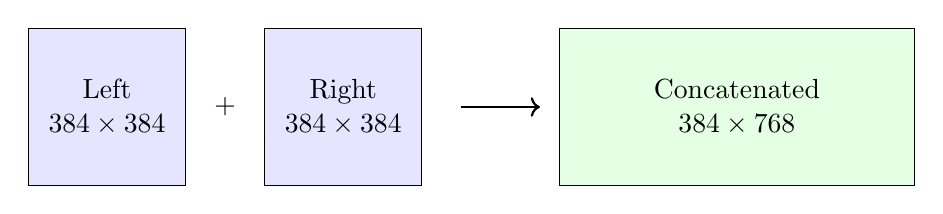
\begin{tikzpicture}[
        img/.style={rectangle, draw, minimum width=2cm, minimum height=2cm, align=center},
        arrow/.style={->, thick}
    ]
        \node[img, fill=blue!10] (left) at (0,0) {Left\\$384 \times 384$};
        \node[img, fill=blue!10] (right) at (3,0) {Right\\$384 \times 384$};
        \node at (1.5,0) {$+$};
        \node[img, fill=green!10, minimum width=4.5cm] (concat) at (8,0) {Concatenated\\$384 \times 768$};

        \draw[arrow] (4.5,0) -- (5.5,0);
    \end{tikzpicture}
    \end{center}

    \begin{block}{Camera Order}
        Left image $\rightarrow$ Right image (spatial alignment)
    \end{block}
\end{frame}

%------------------------------------------------------------------------------
\begin{frame}{Image Input Processing (2/2)}
    \textbf{Processing Steps:}
    \begin{enumerate}
        \item Camera captures at $1280 \times 1024$
        \item Resize to $384 \times 384$ per camera
        \item Concatenate horizontally: $384 \times 768 \times 3$
        \item Optional JPEG compression (training augmentation)
    \end{enumerate}
\end{frame}

%------------------------------------------------------------------------------
\begin{frame}[fragile]{Chat Template Format (1/2)}
    \textbf{Qwen2.5-VL Chat Structure:}

    \vspace{0.3cm}
    \begin{lstlisting}[language=Python]
messages = [{
    "role": "user",
    "content": [
        {"type": "image", "image": concatenated_image},
        {"type": "text", "text": instruction}
    ]
}]

text = processor.apply_chat_template(
    messages, tokenize=False, add_generation_prompt=True
)
text += "<|im_start|>assistant\n<|quad_start|>"
    \end{lstlisting}
\end{frame}

%------------------------------------------------------------------------------
\begin{frame}{Chat Template Format (2/2)}
    \textbf{Special Tokens:}

    \vspace{0.5cm}
    \begin{table}
        \centering
        \begin{tabular}{ll}
            \toprule
            \textbf{Token} & \textbf{Purpose} \\
            \midrule
            \code{<|im\_start|>} & Message start marker \\
            \code{<|im\_end|>} & Message end marker \\
            \code{<|quad\_start|>} & Action sequence start \\
            \code{<|quad\_end|>} & Action sequence end \\
            \bottomrule
        \end{tabular}
    \end{table}
\end{frame}

%------------------------------------------------------------------------------
\begin{frame}{Token Sequence Structure}
    \textbf{Complete Input Sequence:}

    \vspace{0.3cm}
    \begin{center}
    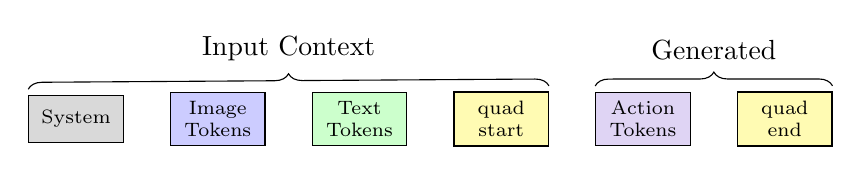
\begin{tikzpicture}[
        tok/.style={rectangle, draw, minimum width=1.2cm, minimum height=0.6cm, align=center, font=\scriptsize},
        arrow/.style={->, thick}
    ]
        \node[tok, fill=gray!30] (sys) at (0,0) {System};
        \node[tok, fill=blue!20] (img) at (1.8,0) {Image\\Tokens};
        \node[tok, fill=green!20] (text) at (3.6,0) {Text\\Tokens};
        \node[tok, fill=yellow!30] (start) at (5.4,0) {quad\\start};
        \node[tok, fill=vqpurple!30] (act) at (7.2,0) {Action\\Tokens};
        \node[tok, fill=yellow!30] (end) at (9,0) {quad\\end};

        \draw[decorate, decoration={brace, amplitude=5pt, raise=2pt}]
            (sys.north west) -- (start.north east) node[midway, above=8pt] {Input Context};

        \draw[decorate, decoration={brace, amplitude=5pt, raise=2pt}]
            (act.north west) -- (end.north east) node[midway, above=8pt] {Generated};
    \end{tikzpicture}
    \end{center}

    \vspace{0.5cm}
    \textbf{Token Counts:}
    \begin{itemize}
        \item Image tokens: $\sim$1000 (depends on resolution)
        \item Text tokens: Variable (instruction length)
        \item Action tokens: Exactly 27
        \item Total context: $< 2048$ tokens
    \end{itemize}
\end{frame}

%------------------------------------------------------------------------------
\begin{frame}{Autoregressive Generation (1/2)}
    \begin{block}{Process}
        Generate 27 action tokens one at a time
    \end{block}

    \vspace{0.3cm}
    \textbf{Generation Loop:}
    \begin{algorithmic}[1]
        \State $\vect{h} \leftarrow \text{Encode}(\text{image}, \text{instruction})$
        \State $\vect{t} \leftarrow [\;]$ \Comment{token sequence}
        \For{$i = 1$ to $27$}
            \State $p_i \leftarrow \text{LMHead}(\vect{h})$ \Comment{logits over vocabulary}
            \State $t_i \leftarrow \argmax(p_i)$ \Comment{greedy decoding}
            \State $\vect{t}.\text{append}(t_i)$
            \State $\vect{h} \leftarrow \text{Update}(\vect{h}, t_i)$ \Comment{KV cache update}
        \EndFor
        \State \textbf{Return} $\vect{t}$
    \end{algorithmic}
\end{frame}

%------------------------------------------------------------------------------
\begin{frame}{Autoregressive Generation (2/2)}
    \textbf{Inference Configuration:}
    \begin{itemize}
        \item Temperature: $0.0$ (greedy decoding)
        \item Max tokens: 29 (27 action + 2 markers)
        \item Sampling: Deterministic (argmax)
    \end{itemize}

    \vspace{0.5cm}
    \begin{alertblock}{Computational Cost}
        \begin{itemize}
            \item 27 sequential forward passes required
            \item Cannot parallelize (autoregressive dependency)
            \item KV cache reduces redundant computation
        \end{itemize}
    \end{alertblock}
\end{frame}

%------------------------------------------------------------------------------
\begin{frame}{Autoregressive Token Generation: Visual Timeline}
    \begin{center}
    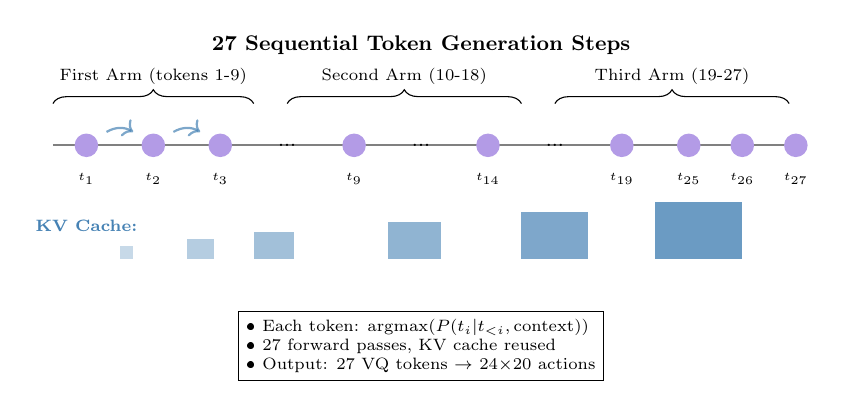
\begin{tikzpicture}[scale=0.85, transform shape]
        % Title for timeline
        \node[font=\small\bfseries] at (0,3) {27 Sequential Token Generation Steps};

        % Timeline base
        \draw[thick, gray] (-5.5,1.5) -- (5.5,1.5);

        % Token generation steps - show 9 representative tokens
        \foreach \i/\x/\label in {1/-5/t_1, 2/-4/t_2, 3/-3/t_3, 9/-1/t_9, 14/1/t_{14}, 19/3/t_{19}, 25/4/t_{25}, 26/4.8/t_{26}, 27/5.6/t_{27}} {
            % Token circle
            \fill[vqpurple!70] (\x,1.5) circle (5pt);
            \node[font=\tiny, below] at (\x,1.2) {$\label$};
        }

        % Ellipsis for skipped tokens
        \node[font=\small] at (-2,1.5) {...};
        \node[font=\small] at (0,1.5) {...};
        \node[font=\small] at (2,1.5) {...};

        % Arrows showing autoregressive dependency
        \draw[->, thick, qwenblue, opacity=0.7] (-4.7,1.7) to[bend left=30] (-4.3,1.7);
        \draw[->, thick, qwenblue, opacity=0.7] (-3.7,1.7) to[bend left=30] (-3.3,1.7);

        % KV Cache accumulation visualization
        \node[font=\scriptsize\bfseries, qwenblue] at (-5,0.3) {KV Cache:};

        % Growing KV cache bars
        \fill[qwenblue!30] (-4.5,-0.2) rectangle (-4.3,0);
        \fill[qwenblue!40] (-3.5,-0.2) rectangle (-3.1,0.1);
        \fill[qwenblue!50] (-2.5,-0.2) rectangle (-1.9,0.2);
        \fill[qwenblue!60] (-0.5,-0.2) rectangle (0.3,0.35);
        \fill[qwenblue!70] (1.5,-0.2) rectangle (2.5,0.5);
        \fill[qwenblue!80] (3.5,-0.2) rectangle (4.8,0.65);

        % Labels for phases
        \draw[decorate, decoration={brace, amplitude=5pt, raise=3pt}] (-5.5,2) -- (-2.5,2)
            node[midway, above=8pt, font=\scriptsize] {First Arm (tokens 1-9)};
        \draw[decorate, decoration={brace, amplitude=5pt, raise=3pt}] (-2,2) -- (1.5,2)
            node[midway, above=8pt, font=\scriptsize] {Second Arm (10-18)};
        \draw[decorate, decoration={brace, amplitude=5pt, raise=3pt}] (2,2) -- (5.5,2)
            node[midway, above=8pt, font=\scriptsize] {Third Arm (19-27)};

        % Legend
        \node[draw, fill=white, font=\scriptsize, align=left] at (0,-1.5) {
            \textbullet\ Each token: argmax($P(t_i | t_{<i}, \text{context})$)\\
            \textbullet\ 27 forward passes, KV cache reused\\
            \textbullet\ Output: 27 VQ tokens $\rightarrow$ 24$\times$20 actions
        };
    \end{tikzpicture}
    \end{center}
\end{frame}

%------------------------------------------------------------------------------
\begin{frame}[fragile]{Token to Action Conversion (1/2)}
    \textbf{Step 1: Extract Action Tokens}
    \begin{lstlisting}[language=Python]
# Find markers in generated sequence
quad_start = find_token(output, "<|quad_start|>")
quad_end = find_token(output, "<|quad_end|>")
action_tokens = output[quad_start+1 : quad_end]
    \end{lstlisting}

    \vspace{0.3cm}
    \textbf{Step 2: Convert VLA $\rightarrow$ VAE Token IDs}
    \begin{lstlisting}[language=Python]
vocab_size = 152064
vae_tokens = vocab_size - (action_tokens + 1)
vae_tokens = vae_tokens.clamp(0, 1023)
    \end{lstlisting}
\end{frame}

%------------------------------------------------------------------------------
\begin{frame}[fragile]{Token to Action Conversion (2/2)}
    \textbf{Step 3: Decode via VQVAE}
    \begin{lstlisting}[language=Python]
actions = vae.decode(vae_tokens)  # [B, 24, 20]
    \end{lstlisting}

    \vspace{0.3cm}
    \textbf{Step 4: Unnormalize}
    \begin{lstlisting}[language=Python]
actions = normalizer["action"].unnormalize(actions)
    \end{lstlisting}

    \vspace{0.5cm}
    \begin{block}{Output Specification}
        \begin{itemize}
            \item Shape: $[B, 24, 20]$ (batch, timesteps, action\_dim)
            \item Units: Physical coordinates (meters, radians, binary)
        \end{itemize}
    \end{block}
\end{frame}

%------------------------------------------------------------------------------
\begin{frame}{Valid Token Rate (1/2)}
    \begin{block}{Quality Metric}
        Percentage of generated tokens within valid codebook range
    \end{block}

    \vspace{0.3cm}
    \textbf{Definition:}
    \[
        \text{valid\_rate} = \frac{|\{t : 0 \leq t < 1024\}|}{27}
    \]

    \vspace{0.3cm}
    \textbf{Invalid Token Causes:}
    \begin{itemize}
        \item Model generates text tokens instead of action tokens
        \item Token ID outside codebook range after conversion
        \item Premature \code{<|quad\_end|>} generation
    \end{itemize}
\end{frame}

%------------------------------------------------------------------------------
\begin{frame}{Valid Token Rate (2/2)}
    \begin{alertblock}{Handling Invalid Tokens}
        \begin{itemize}
            \item Clamp to valid range: $[0, 1023]$
            \item Monitor valid\_rate during training/inference
            \item Low valid\_rate indicates training issues
        \end{itemize}
    \end{alertblock}

    \vspace{0.5cm}
    \begin{block}{Expected Values}
        \begin{itemize}
            \item Well-trained model: $> 99\%$ valid rate
            \item Early training: May have lower valid rate
            \item Zero-shot: Varies by embodiment similarity
        \end{itemize}
    \end{block}
\end{frame}

%------------------------------------------------------------------------------
\begin{frame}{Training: Loss Function}
    \textbf{Cross-Entropy Loss on Action Tokens:}

    \vspace{0.3cm}
    \[
        \mathcal{L}_{\text{CE}} = -\sum_{i=1}^{27} \log P(t_i | t_{<i}, \text{image}, \text{instruction})
    \]

    \vspace{0.5cm}
    \textbf{Label Preparation:}
    \begin{enumerate}
        \item Encode ground-truth actions: $\vect{a} \rightarrow \vect{t}_{\text{gt}}$ via VQVAE
        \item Convert to VLA token IDs: $t_{\text{vla}} = V - t_{\text{vae}} - 1$
        \item Mask non-action positions: $-100$ (ignored in loss)
    \end{enumerate}

    \vspace{0.3cm}
    \textbf{Training Configuration:}
    \begin{itemize}
        \item Only action token positions contribute to loss
        \item Image/text tokens are input context only
        \item Teacher forcing: ground-truth tokens as input
    \end{itemize}
\end{frame}

%------------------------------------------------------------------------------
\begin{frame}[fragile]{Training: LoRA Configuration (1/2)}
    \begin{block}{Parameter-Efficient Fine-Tuning}
        LoRA adapters on attention layers
    \end{block}

    \vspace{0.3cm}
    \textbf{Target Modules:}
    \begin{lstlisting}[language=Python]
LoraConfig(
    r=8,                    # LoRA rank
    lora_alpha=8,           # Scaling factor
    lora_dropout=0.1,       # Dropout rate
    target_modules=[
        "q_proj", "k_proj", "v_proj", "o_proj",
        "gate_proj", "up_proj", "down_proj"
    ],
    use_dora=False,
    init_lora_weights="gaussian"
)
    \end{lstlisting}
\end{frame}

%------------------------------------------------------------------------------
\begin{frame}{Training: LoRA Configuration (2/2)}
    \textbf{Trainable Parameters:}
    \begin{itemize}
        \item LoRA: $\sim$20M parameters (0.3\% of 7B)
        \item Full fine-tune: 7B parameters
    \end{itemize}

    \vspace{0.5cm}
    \begin{block}{LoRA Benefits}
        \begin{itemize}
            \item Reduces memory: 80GB $\rightarrow$ 32GB
            \item Faster training convergence
            \item Preserves base model capabilities
            \item Easy to merge or swap adapters
        \end{itemize}
    \end{block}
\end{frame}

%------------------------------------------------------------------------------
\begin{frame}[fragile]{Training: QLoRA Configuration}
    \begin{columns}[T]
        \begin{column}{0.55\textwidth}
            \begin{block}{Quantized LoRA}
                4-bit quantization + LoRA
            \end{block}

            \vspace{0.2cm}
            \textbf{BitsAndBytes Config:}
            \begin{lstlisting}[language=Python]
BitsAndBytesConfig(
    load_in_4bit=True,
    bnb_4bit_use_double_quant=True,
    bnb_4bit_quant_type="nf4",
    bnb_4bit_compute_dtype=bfloat16
)
            \end{lstlisting}
        \end{column}
        \begin{column}{0.45\textwidth}
            \textbf{LoRA + DoRA:}
            \begin{lstlisting}[language=Python]
LoraConfig(
    use_dora=True
)
            \end{lstlisting}

            \vspace{0.2cm}
            \textbf{Memory:}
            \begin{itemize}
                \item Full: 80GB
                \item LoRA: 32GB
                \item QLoRA: 20GB
            \end{itemize}
        \end{column}
    \end{columns}
\end{frame}

%------------------------------------------------------------------------------
\begin{frame}{Evaluation Metrics (1/2)}
    \textbf{Computed during training/validation:}

    \vspace{0.5cm}
    \begin{table}
        \centering
        \renewcommand{\arraystretch}{1.3}
        \begin{tabular}{ll}
            \toprule
            \textbf{Metric} & \textbf{Formula} \\
            \midrule
            Valid Rate & $\frac{\text{\# valid tokens}}{27}$ \\[0.3cm]
            MSE (Total) & $\|\hat{\vect{a}} - \vect{a}\|^2$ \\[0.3cm]
            MSE (Position) & $\|\hat{\vect{p}} - \vect{p}\|^2$ \\
            \bottomrule
        \end{tabular}
    \end{table}
\end{frame}

%------------------------------------------------------------------------------
\begin{frame}{Evaluation Metrics (2/2)}
    \begin{table}
        \centering
        \renewcommand{\arraystretch}{1.3}
        \begin{tabular}{ll}
            \toprule
            \textbf{Metric} & \textbf{Formula} \\
            \midrule
            Geodesic (Rotation) & $\arccos\left(\frac{\text{tr}(\mat{R}^T \hat{\mat{R}}) - 1}{2}\right)$ \\[0.3cm]
            MSE (Gripper) & $\|\hat{g} - g\|^2$ \\
            \bottomrule
        \end{tabular}
    \end{table}

    \vspace{0.5cm}
    \begin{block}{Note}
        Metrics computed on unnormalized actions for interpretability
    \end{block}
\end{frame}

%------------------------------------------------------------------------------
\begin{frame}[fragile]{vLLM Acceleration (1/2)}
    \begin{block}{Purpose}
        Faster inference using optimized LLM serving
    \end{block}

    \vspace{0.3cm}
    \textbf{vLLM Configuration:}
    \begin{lstlisting}[language=Python]
from vllm import LLM, SamplingParams

llm = LLM(
    model=model_path,
    dtype=torch.bfloat16,
    tensor_parallel_size=1,
    enable_chunked_prefill=True,
    gpu_memory_utilization=0.90,
    max_model_len=2048,
    limit_mm_per_prompt={"image": 1}
)
    \end{lstlisting}
\end{frame}

%------------------------------------------------------------------------------
\begin{frame}[fragile]{vLLM Acceleration (2/2)}
    \textbf{Sampling Parameters:}
    \begin{lstlisting}[language=Python]
sampling_params = SamplingParams(
    max_tokens=29,
    temperature=0.0
)
    \end{lstlisting}

    \vspace{0.5cm}
    \begin{block}{Key vLLM Features}
        \begin{itemize}
            \item Continuous batching
            \item Paged attention (efficient KV cache)
            \item Chunked prefill for long prompts
            \item Multi-modal support
        \end{itemize}
    \end{block}
\end{frame}

%------------------------------------------------------------------------------
\begin{frame}[fragile]{vLLM Inference (1/2)}
    \textbf{Inference with vLLM:}

    \vspace{0.3cm}
    \begin{lstlisting}[language=Python]
# Prepare input
prompt = build_chat_template(image, instruction)

# Generate
outputs = llm.generate(
    prompts=[prompt],
    sampling_params=sampling_params,
    use_tqdm=False
)

# Extract tokens (no detokenization)
token_ids = outputs[0].outputs[0].token_ids
    \end{lstlisting}
\end{frame}

%------------------------------------------------------------------------------
\begin{frame}{vLLM Inference (2/2)}
    \textbf{Performance Comparison:}
    \begin{itemize}
        \item Standard HuggingFace: $\sim$400ms per inference
        \item vLLM: $\sim$237ms per inference
        \item Speedup: $\sim$1.7$\times$
    \end{itemize}

    \vspace{0.5cm}
    \begin{alertblock}{Real-Time Feasibility}
        \begin{itemize}
            \item Action chunk: 0.8s (24 frames at 30Hz)
            \item vLLM inference: 237ms
            \item Ratio: 30\% of chunk duration
            \item \textbf{Real-time capable} with temporal action chunking
        \end{itemize}
    \end{alertblock}
\end{frame}

%------------------------------------------------------------------------------
\begin{frame}[fragile]{KV Cache Optimization}
    \begin{columns}[T]
        \begin{column}{0.45\textwidth}
            \begin{block}{Key Insight}
                Encoding is constant across tokens
            \end{block}

            \vspace{0.2cm}
            \textbf{Standard:}
            \begin{itemize}
                \item $27 \times$ full forward
            \end{itemize}

            \textbf{With KV Cache:}
            \begin{itemize}
                \item 1st: Full forward
                \item 2-27: Decode only
            \end{itemize}
        \end{column}
        \begin{column}{0.55\textwidth}
            \textbf{Implementation:}
            \begin{lstlisting}[language=Python]
# Initial encoding
out = model(**inputs, use_cache=True)
kv = out.past_key_values

# Subsequent generation
out = model(input_ids=new_token,
            past_key_values=kv)
            \end{lstlisting}
        \end{column}
    \end{columns}
\end{frame}

%------------------------------------------------------------------------------
\begin{frame}{RDT2-VQ Strengths \& Weaknesses}
    \begin{columns}[T]
        \begin{column}{0.5\textwidth}
            \textbf{Strengths:}
            \begin{itemize}
                \item Full VLM language understanding
                \item Superior instruction following
                \item Unified text-action interface
                \item Stable discrete training
                \item Leverages pretrained VLM
            \end{itemize}
        \end{column}
        \begin{column}{0.5\textwidth}
            \textbf{Weaknesses:}
            \begin{itemize}
                \item 27 forward passes (slow)
                \item Discretization error
                \item High memory usage
                \item Sequential generation
                \item Cannot parallelize tokens
            \end{itemize}
        \end{column}
    \end{columns}

    \vspace{0.5cm}
    \begin{alertblock}{Latency Analysis}
        27 forward passes $\times$ $\sim$15ms = $\sim$400ms per action chunk \\
        Action chunk = 0.8s $\Rightarrow$ \textbf{50\% of real-time}
    \end{alertblock}
\end{frame}

%------------------------------------------------------------------------------
\begin{frame}[fragile]{HuggingFace Model}
    \textbf{Model:} \code{robotics-diffusion-transformer/RDT2-VQ}

    \vspace{0.3cm}
    \textbf{Loading:}
    \begin{lstlisting}[language=Python]
from transformers import (
    Qwen2_5_VLForConditionalGeneration, AutoProcessor
)

model = Qwen2_5_VLForConditionalGeneration.from_pretrained(
    "robotics-diffusion-transformer/RDT2-VQ",
    torch_dtype=torch.bfloat16,
    attn_implementation="flash_attention_2"
)

processor = AutoProcessor.from_pretrained(
    "Qwen/Qwen2.5-VL-7B-Instruct"
)
    \end{lstlisting}
\end{frame}

%------------------------------------------------------------------------------
\begin{frame}{Complete Inference Pipeline}
    \begin{center}
    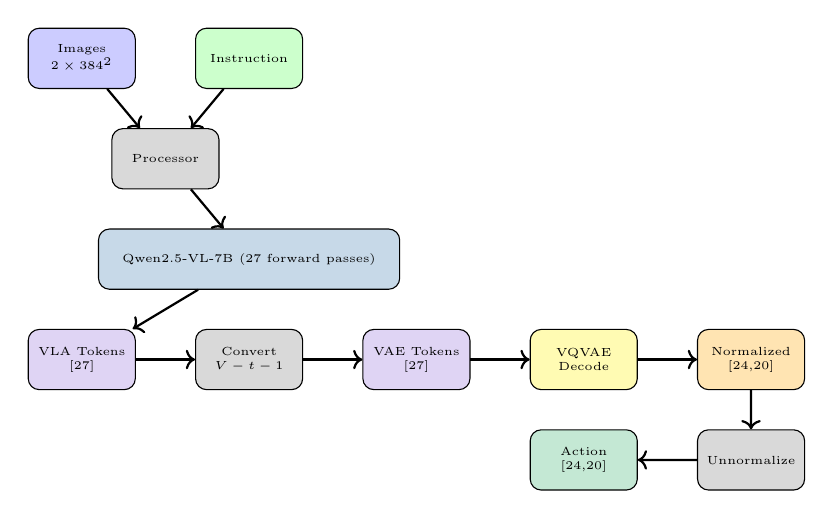
\begin{tikzpicture}[
        box/.style={rectangle, draw, rounded corners, minimum width=1.6cm, minimum height=0.9cm, align=center, font=\tiny},
        arrow/.style={->, thick},
        scale=0.85, transform shape
    ]
        % Row 1: Input (Images and Instruction side by side)
        \node[box, fill=blue!20] (img) at (0,3.5) {Images\\$2 \times 384^2$};
        \node[box, fill=green!20] (inst) at (2.5,3.5) {Instruction};

        % Processor below inputs
        \node[box, fill=gray!30] (proc) at (1.25,2) {Processor};

        % Row 2: Model
        \node[box, fill=qwenblue!30, minimum width=4.5cm] (qwen) at (2.5,0.5) {Qwen2.5-VL-7B (27 forward passes)};

        % Row 3: Tokens
        \node[box, fill=vqpurple!30] (vla_tok) at (0,-1) {VLA Tokens\\{[}27{]}};
        \node[box, fill=gray!30] (convert) at (2.5,-1) {Convert\\$V - t - 1$};
        \node[box, fill=vqpurple!30] (vae_tok) at (5,-1) {VAE Tokens\\{[}27{]}};
        \node[box, fill=yellow!30] (vae) at (7.5,-1) {VQVAE\\Decode};
        \node[box, fill=actionorange!30] (norm_act) at (10,-1) {Normalized\\{[}24,20{]}};

        % Row 4: Output
        \node[box, fill=gray!30] (unnorm) at (10,-2.5) {Unnormalize};
        \node[box, fill=rdtgreen!30] (action) at (7.5,-2.5) {Action\\{[}24,20{]}};

        % Arrows - Images and Instruction both go to Processor
        \draw[arrow] (img) -- (proc);
        \draw[arrow] (inst) -- (proc);
        \draw[arrow] (proc) -- (qwen);
        \draw[arrow] (qwen) -- (vla_tok);
        \draw[arrow] (vla_tok) -- (convert);
        \draw[arrow] (convert) -- (vae_tok);
        \draw[arrow] (vae_tok) -- (vae);
        \draw[arrow] (vae) -- (norm_act);
        \draw[arrow] (norm_act) -- (unnorm);
        \draw[arrow] (unnorm) -- (action);
    \end{tikzpicture}
    \end{center}

    \vspace{0.3cm}
    \textbf{Total Latency:} $\sim$400ms (without vLLM) / $\sim$237ms (with vLLM)
\end{frame}

%------------------------------------------------------------------------------
\begin{frame}{RDT2-VQ Summary (1/2)}
    \begin{table}
        \centering
        \renewcommand{\arraystretch}{1.3}
        \begin{tabular}{ll}
            \toprule
            \textbf{Attribute} & \textbf{Value} \\
            \midrule
            Backbone & Qwen2.5-VL-7B-Instruct \\
            Output type & Discrete tokens \\
            Tokens per chunk & 27 \\
            Forward passes & 27 \\
            Action chunk & 24 frames (0.8s) \\
            \bottomrule
        \end{tabular}
    \end{table}
\end{frame}

%------------------------------------------------------------------------------
\begin{frame}{RDT2-VQ Summary (2/2)}
    \textbf{Latency:} $\sim$400ms (standard) / $\sim$237ms (with vLLM)

    \vspace{0.5cm}
    \textbf{Training modes:} Full / LoRA / QLoRA

    \vspace{0.5cm}
    \begin{block}{Use Case}
        Best for tasks requiring strong language understanding and instruction following, where latency is acceptable
    \end{block}
\end{frame}


% %==============================================================================
% PART 5: RDT2-FM ARCHITECTURE
%==============================================================================

\section{RDT2-FM Architecture}

%------------------------------------------------------------------------------
\begin{frame}{RDT2-FM Overview}
    \begin{block}{Definition}
        \textbf{RDT2-FM} = Frozen VLM + Flow-Matching Action Expert
    \end{block}

    \vspace{0.5cm}
    \textbf{Core Architecture:}
    \begin{itemize}
        \item \textbf{VLM Backbone:} Qwen2.5-VL-7B-Instruct (\textbf{frozen})
        \item \textbf{Action Expert:} 400M parameter RDT transformer
        \item \textbf{Generation:} Flow-matching diffusion (5 steps)
    \end{itemize}

    \vspace{0.5cm}
    \begin{alertblock}{Key Advantage}
        \textbf{6 forward passes} total (1 VLM + 5 RDT) \\
        $\sim$4.5$\times$ faster than RDT2-VQ
    \end{alertblock}
\end{frame}

%------------------------------------------------------------------------------
\begin{frame}{Architecture Comparison}
    \begin{table}
        \centering
        \renewcommand{\arraystretch}{1.4}
        \begin{tabular}{lcc}
            \toprule
            & \textbf{RDT2-VQ} & \textbf{RDT2-FM} \\
            \midrule
            VLM Backbone & Fine-tuned & \textbf{Frozen} \\
            Action Output & Discrete (27 tokens) & \textbf{Continuous} \\
            Forward Passes & 27 & \textbf{6} \\
            Trainable Params & 7B+ & \textbf{400M} \\
            Training VRAM & $\geq$32 GB & \textbf{$\sim$16 GB} \\
            \bottomrule
        \end{tabular}
    \end{table}

    \vspace{0.5cm}
    \begin{block}{Key Insight}
        Freeze VLM $\rightarrow$ Only train lightweight action expert \\
        Same visual understanding, much faster training
    \end{block}
\end{frame}

%------------------------------------------------------------------------------
\begin{frame}{RDT2-FM Architecture Diagram}
    \begin{center}
    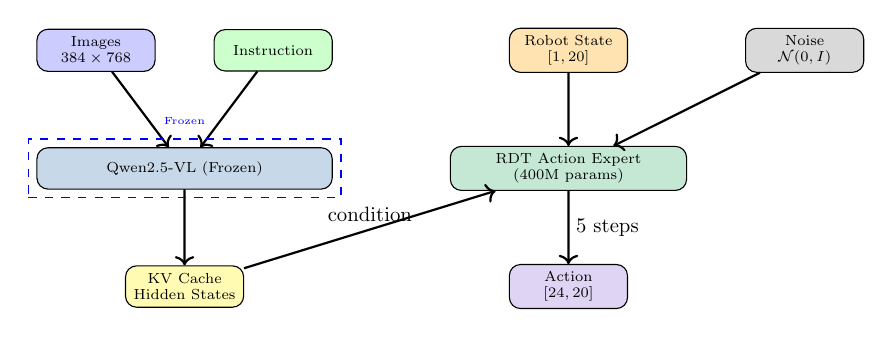
\begin{tikzpicture}[
        box/.style={rectangle, draw, rounded corners, minimum width=2cm, minimum height=0.7cm, align=center, font=\scriptsize},
        arrow/.style={->, thick},
        scale=0.75, transform shape
    ]
        % Input
        \node[box, fill=blue!20] (img) at (0,4) {Images\\$384 \times 768$};
        \node[box, fill=green!20] (inst) at (3,4) {Instruction};

        % Frozen VLM
        \node[box, fill=qwenblue!30, minimum width=5cm] (qwen) at (1.5,2) {Qwen2.5-VL (Frozen)};
        \node[box, fill=yellow!30] (kv) at (1.5,0) {KV Cache\\Hidden States};

        % RDT Expert
        \node[box, fill=rdtgreen!30, minimum width=4cm] (rdt) at (8,2) {RDT Action Expert\\(400M params)};

        % State input
        \node[box, fill=actionorange!30] (state) at (8,4) {Robot State\\$[1, 20]$};

        % Noise
        \node[box, fill=gray!30] (noise) at (12,4) {Noise\\$\mathcal{N}(0, I)$};

        % Output
        \node[box, fill=vqpurple!30] (action) at (8,0) {Action\\$[24, 20]$};

        % Arrows
        \draw[arrow] (img) -- (qwen);
        \draw[arrow] (inst) -- (qwen);
        \draw[arrow] (qwen) -- (kv);
        \draw[arrow] (kv) -- node[above] {condition} (rdt);
        \draw[arrow] (state) -- (rdt);
        \draw[arrow] (noise) -- (rdt);
        \draw[arrow] (rdt) -- node[right] {5 steps} (action);

        % Frozen indicator
        \node[draw, dashed, blue, fit=(qwen), inner sep=3pt] {};
        \node[blue, font=\tiny] at (1.5,2.8) {Frozen};
    \end{tikzpicture}
    \end{center}
\end{frame}

%------------------------------------------------------------------------------
\begin{frame}{Flow Matching: Overview (1/2)}
    \begin{block}{Core Idea}
        Learn to transport samples from noise distribution to data distribution
    \end{block}

    \vspace{0.3cm}
    \textbf{Probability Flow ODE:}
    \[
        \frac{d\vect{x}_t}{dt} = \vect{v}_\theta(\vect{x}_t, t)
    \]

    where $\vect{v}_\theta$ is the learned velocity field
\end{frame}

%------------------------------------------------------------------------------
\begin{frame}{Flow Matching: Overview (2/2)}
    \textbf{Interpolation Path (Linear):}
    \[
        \vect{x}_t = (1 - t) \cdot \vect{x}_0 + t \cdot \vect{x}_1
    \]

    \begin{itemize}
        \item $t = 0$: Pure noise $\vect{x}_0 \sim \mathcal{N}(0, I)$
        \item $t = 1$: Data sample $\vect{x}_1 = \vect{a}_{\text{gt}}$
    \end{itemize}

    \vspace{0.3cm}
    \textbf{Target Velocity:}
    \[
        \vect{v}^* = \vect{x}_1 - \vect{x}_0 = \vect{a}_{\text{gt}} - \boldsymbol{\epsilon}
    \]
\end{frame}

%------------------------------------------------------------------------------
\begin{frame}{Flow Matching: Noise to Data Trajectory}
    \begin{center}
    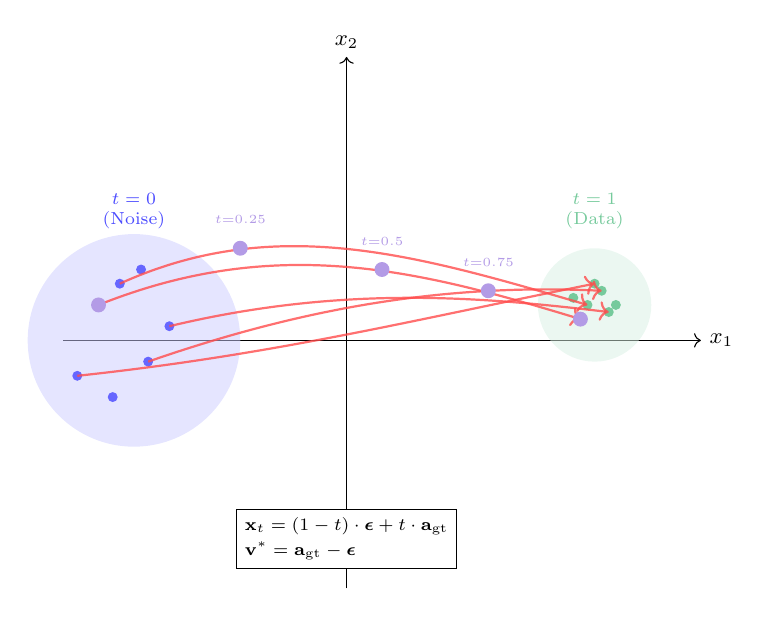
\begin{tikzpicture}[scale=0.9, transform shape]
        % Axes
        \draw[->] (-4,0) -- (5,0) node[right, font=\small] {$x_1$};
        \draw[->] (0,-3.5) -- (0,4) node[above, font=\small] {$x_2$};

        % Noise distribution (t=0) - scattered points on left
        \begin{scope}
            \fill[blue!20, opacity=0.5] (-3,0) circle (1.5);
            \node[blue!70, font=\scriptsize] at (-3,2) {$t=0$};
            \node[blue!70, font=\scriptsize] at (-3,1.7) {(Noise)};

            % Sample points from noise
            \foreach \x/\y in {-3.5/0.5, -2.8/-0.3, -3.2/0.8, -2.5/0.2, -3.8/-0.5, -2.9/1.0, -3.3/-0.8} {
                \fill[blue!60] (\x,\y) circle (2pt);
            }
        \end{scope}

        % Data distribution (t=1) - clustered on right
        \begin{scope}
            \fill[rdtgreen!20, opacity=0.5] (3.5,0.5) circle (0.8);
            \node[rdtgreen!70, font=\scriptsize] at (3.5,2) {$t=1$};
            \node[rdtgreen!70, font=\scriptsize] at (3.5,1.7) {(Data)};

            % Target data points
            \foreach \x/\y in {3.3/0.3, 3.6/0.7, 3.4/0.5, 3.7/0.4, 3.5/0.8, 3.2/0.6, 3.8/0.5} {
                \fill[rdtgreen!70] (\x,\y) circle (2pt);
            }
        \end{scope}

        % Flow trajectories (curved arrows from noise to data)
        \draw[->, thick, red!70, opacity=0.8] (-3.5,0.5)
            .. controls (-1,1.5) and (1,1) .. (3.3,0.3);
        \draw[->, thick, red!70, opacity=0.8] (-2.8,-0.3)
            .. controls (-0.5,0.5) and (1.5,0.8) .. (3.6,0.7);
        \draw[->, thick, red!70, opacity=0.8] (-3.2,0.8)
            .. controls (-1,1.8) and (1,1.2) .. (3.4,0.5);
        \draw[->, thick, red!70, opacity=0.8] (-2.5,0.2)
            .. controls (0,0.8) and (2,0.6) .. (3.7,0.4);
        \draw[->, thick, red!70, opacity=0.8] (-3.8,-0.5)
            .. controls (-1,-0.2) and (1,0.3) .. (3.5,0.8);

        % Time markers along one trajectory
        \fill[vqpurple!70] (-3.5,0.5) circle (3pt);
        \fill[vqpurple!70] (-1.5,1.3) circle (3pt);
        \fill[vqpurple!70] (0.5,1.0) circle (3pt);
        \fill[vqpurple!70] (2,0.7) circle (3pt);
        \fill[vqpurple!70] (3.3,0.3) circle (3pt);

        \node[vqpurple!70, font=\tiny] at (-1.5,1.7) {$t{=}0.25$};
        \node[vqpurple!70, font=\tiny] at (0.5,1.4) {$t{=}0.5$};
        \node[vqpurple!70, font=\tiny] at (2,1.1) {$t{=}0.75$};

        % Legend / Equation
        \node[draw, fill=white, font=\scriptsize, align=left] at (0,-2.8) {
            $\mathbf{x}_t = (1-t)\cdot\boldsymbol{\epsilon} + t\cdot\mathbf{a}_{\text{gt}}$\\[2pt]
            $\mathbf{v}^* = \mathbf{a}_{\text{gt}} - \boldsymbol{\epsilon}$
        };
    \end{tikzpicture}
    \end{center}
\end{frame}

%------------------------------------------------------------------------------
\begin{frame}{Flow Matching: Training Loss}
    \textbf{Objective: Learn to predict velocity}

    \vspace{0.5cm}
    \textbf{Training Procedure:}
    \begin{enumerate}
        \item Sample noise: $\boldsymbol{\epsilon} \sim \mathcal{N}(0, I)$
        \item Sample timestep: $t \sim \text{LogisticNormal}(\mu, \sigma)$
        \item Create noisy action: $\vect{a}_t = (1 - t) \cdot \boldsymbol{\epsilon} + t \cdot \vect{a}_{\text{gt}}$
        \item Predict velocity: $\hat{\vect{v}} = f_\theta(\vect{a}_t, t, \text{cond})$
        \item Compute loss: $\mathcal{L} = \|\hat{\vect{v}} - (\vect{a}_{\text{gt}} - \boldsymbol{\epsilon})\|^2$
    \end{enumerate}

    \vspace{0.5cm}
    \textbf{Flow Matching Loss:}
    \[
        \boxed{\mathcal{L}_{\text{FM}} = \mathbb{E}_{t, \boldsymbol{\epsilon}, \vect{a}} \left[ \| \vect{v}_\theta(\vect{a}_t, t) - (\vect{a} - \boldsymbol{\epsilon}) \|^2 \right]}
    \]
\end{frame}

%------------------------------------------------------------------------------
\begin{frame}{Timestep Sampling: Logistic Normal (1/2)}
    \begin{block}{Why Not Uniform?}
        Different timesteps have different importance for learning
    \end{block}

    \vspace{0.3cm}
    \textbf{Logistic Normal Distribution:}
    \[
        t = \sigma\left(\frac{u - \mu}{\sigma}\right), \quad u \sim \mathcal{N}(0, 1)
    \]

    where $\sigma(x) = \frac{1}{1 + e^{-x}}$ (sigmoid)
\end{frame}

%------------------------------------------------------------------------------
\begin{frame}{Timestep Sampling: Logistic Normal (2/2)}
    \textbf{Default Parameters:}
    \begin{itemize}
        \item $\mu = 0$ (center)
        \item $\sigma = 1$ (spread)
    \end{itemize}

    \vspace{0.3cm}
    \begin{alertblock}{Effect}
        More samples near $t = 0.5$ (intermediate states) \\
        Fewer samples at extremes ($t \approx 0$ or $t \approx 1$)
    \end{alertblock}
\end{frame}

%------------------------------------------------------------------------------
\begin{frame}{Inference: Euler Integration}
    \textbf{Generate actions by integrating velocity field}

    \vspace{0.3cm}
    \textbf{Algorithm (5 steps):}
    \begin{algorithmic}[1]
        \State $\vect{a}_0 \sim \mathcal{N}(0, I)$ \Comment{Sample noise}
        \State $\Delta t \leftarrow 1 / N$ \Comment{$N = 5$ steps}
        \For{$i = 0$ to $N-1$}
            \State $t \leftarrow i \cdot \Delta t$
            \State $\vect{v} \leftarrow \vect{v}_\theta(\vect{a}_t, t, \text{cond})$ \Comment{RDT forward}
            \State $\vect{a}_{t + \Delta t} \leftarrow \vect{a}_t + \vect{v} \cdot \Delta t$ \Comment{Euler step}
        \EndFor
        \State \textbf{Return} $\vect{a}_1$
    \end{algorithmic}

    \vspace{0.5cm}
    \textbf{Timesteps:} $t \in \{0, 0.2, 0.4, 0.6, 0.8\} \rightarrow 1.0$
\end{frame}

%------------------------------------------------------------------------------
\begin{frame}{RDT Transformer Architecture}
    \begin{block}{RDT = Robotics Diffusion Transformer}
        Specialized transformer for action diffusion
    \end{block}

    \vspace{0.3cm}
    \textbf{Architecture Specifications:}
    \begin{table}
        \centering
        \renewcommand{\arraystretch}{1.2}
        \begin{tabular}{ll}
            \toprule
            \textbf{Parameter} & \textbf{Value} \\
            \midrule
            Hidden size & 1024 \\
            Depth (layers) & 14 \\
            Attention heads & 8 \\
            KV heads (GQA) & 4 \\
            Register tokens & 4 \\
            FFN multiplier & 256 \\
            Total params & $\sim$400M \\
            \bottomrule
        \end{tabular}
    \end{table}
\end{frame}

%------------------------------------------------------------------------------
\begin{frame}{RDT Block Structure}
    \begin{center}
    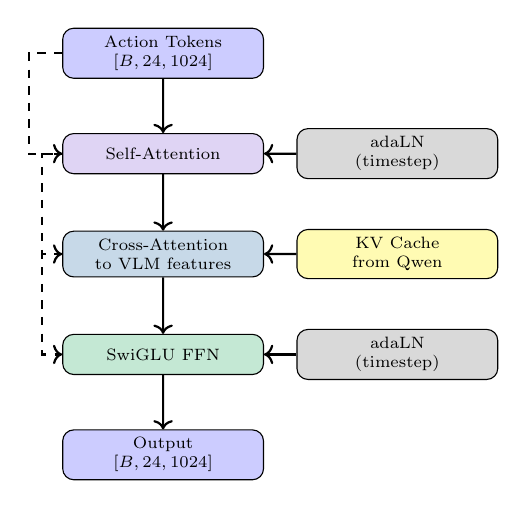
\begin{tikzpicture}[
        box/.style={rectangle, draw, rounded corners, minimum width=3cm, minimum height=0.6cm, align=center, font=\scriptsize},
        arrow/.style={->, thick},
        scale=0.85, transform shape
    ]
        % Input
        \node[box, fill=blue!20] (input) at (0,5) {Action Tokens\\$[B, 24, 1024]$};

        % Self-attention
        \node[box, fill=vqpurple!30] (sa) at (0,3.5) {Self-Attention};
        \node[box, fill=gray!30] (mod1) at (3.5,3.5) {adaLN\\(timestep)};

        % Cross-attention
        \node[box, fill=qwenblue!30] (ca) at (0,2) {Cross-Attention\\to VLM features};
        \node[box, fill=yellow!30] (cond) at (3.5,2) {KV Cache\\from Qwen};

        % FFN
        \node[box, fill=rdtgreen!30] (ffn) at (0,0.5) {SwiGLU FFN};
        \node[box, fill=gray!30] (mod2) at (3.5,0.5) {adaLN\\(timestep)};

        % Output
        \node[box, fill=blue!20] (output) at (0,-1) {Output\\$[B, 24, 1024]$};

        % Arrows
        \draw[arrow] (input) -- (sa);
        \draw[arrow] (mod1) -- (sa);
        \draw[arrow] (sa) -- (ca);
        \draw[arrow] (cond) -- (ca);
        \draw[arrow] (ca) -- (ffn);
        \draw[arrow] (mod2) -- (ffn);
        \draw[arrow] (ffn) -- (output);

        % Residual connections
        \draw[arrow, dashed] (input.west) -- ++(-0.5,0) |- (sa.west);
        \draw[arrow, dashed] (sa.west) -- ++(-0.3,0) |- (ca.west);
        \draw[arrow, dashed] (ca.west) -- ++(-0.3,0) |- (ffn.west);
    \end{tikzpicture}
    \end{center}

    \vspace{0.3cm}
    \textbf{adaLN:} Adaptive Layer Norm modulated by timestep embedding
\end{frame}

%------------------------------------------------------------------------------
\begin{frame}{Timestep Embedding (1/2)}
    \textbf{Sinusoidal Frequency Encoding:}

    \vspace{0.3cm}
    \[
        \text{PE}(t, 2k) = \sin\left(\frac{t}{10000^{2k/d}}\right)
    \]
    \[
        \text{PE}(t, 2k+1) = \cos\left(\frac{t}{10000^{2k/d}}\right)
    \]

    \vspace{0.5cm}
    \textbf{Dimension Flow:}
    \[
        t \in [0, 1] \xrightarrow{\text{sinusoidal}} [256] \xrightarrow{\text{MLP}} [1024]
    \]
\end{frame}

%------------------------------------------------------------------------------
\begin{frame}[fragile]{Timestep Embedding (2/2)}
    \textbf{MLP Processing:}
    \begin{lstlisting}[language=Python]
class TimestepEmbedder(nn.Module):
    def __init__(self, hidden_size, freq_dim=256):
        self.mlp = nn.Sequential(
            nn.Linear(freq_dim, hidden_size),
            nn.SiLU(),
            nn.Linear(hidden_size, hidden_size)
        )
    \end{lstlisting}

    \vspace{0.5cm}
    \begin{block}{Purpose}
        Inject timestep information into each RDT block via adaptive layer norm
    \end{block}
\end{frame}

%------------------------------------------------------------------------------
\begin{frame}{Condition Adaptors}
    \textbf{Project VLM features to RDT hidden space}

    \vspace{0.5cm}
    \begin{center}
    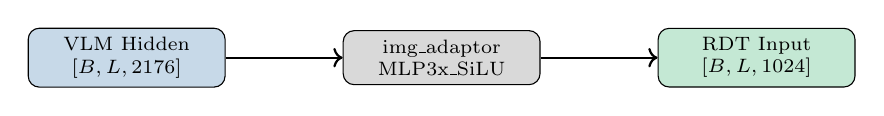
\begin{tikzpicture}[
        box/.style={rectangle, draw, rounded corners, minimum width=2.5cm, minimum height=0.6cm, align=center, font=\scriptsize},
        arrow/.style={->, thick}
    ]
        \node[box, fill=qwenblue!30] (vlm) at (0,0) {VLM Hidden\\$[B, L, 2176]$};
        \node[box, fill=gray!30] (adapt) at (4,0) {img\_adaptor\\MLP3x\_SiLU};
        \node[box, fill=rdtgreen!30] (rdt) at (8,0) {RDT Input\\$[B, L, 1024]$};

        \draw[arrow] (vlm) -- (adapt);
        \draw[arrow] (adapt) -- (rdt);
    \end{tikzpicture}
    \end{center}

    \vspace{0.5cm}
    \textbf{Adaptor Types:}
    \begin{itemize}
        \item \code{mlp2x\_gelu}: $d \rightarrow 2d \rightarrow d$ with GELU
        \item \code{mlp3x\_silu}: $d \rightarrow 3d \rightarrow d$ with SiLU
    \end{itemize}

    \vspace{0.3cm}
    \textbf{Adaptors in RDT:}
    \begin{itemize}
        \item \code{img\_adaptor}: VLM features $\rightarrow$ RDT (2176 $\rightarrow$ 1024)
        \item \code{act\_adaptor}: Action $\rightarrow$ RDT (20 $\rightarrow$ 1024)
        \item \code{state\_adaptor}: State $\rightarrow$ RDT (20 $\rightarrow$ 1024)
    \end{itemize}
\end{frame}

%------------------------------------------------------------------------------
\begin{frame}[fragile]{KV Cache Extraction (1/2)}
    \textbf{Extract VLM hidden states for RDT conditioning}

    \vspace{0.3cm}
    \begin{lstlisting}[language=Python]
# Forward through frozen VLM
with torch.no_grad():
    outputs = vision_language_model(
        **inputs,
        output_hidden_states=True
    )

# Extract selected layer outputs
selected_layers = list(range(14))  # All layers
hidden_states = [
    outputs.hidden_states[i]
    for i in selected_layers
]
    \end{lstlisting}
\end{frame}

%------------------------------------------------------------------------------
\begin{frame}[fragile]{KV Cache Extraction (2/2)}
    \textbf{Stack and create KV cache:}
    \begin{lstlisting}[language=Python]
# Stack and create KV cache
kv_cache = torch.stack(hidden_states, dim=1)
# Shape: [B, num_layers, seq_len, hidden_dim]
    \end{lstlisting}

    \vspace{0.5cm}
    \textbf{VLM Hidden Dim:} 2176 (Qwen2.5-VL specific)

    \vspace{0.3cm}
    \begin{block}{Note}
        All 14 layers are used for conditioning the RDT action expert
    \end{block}
\end{frame}

%------------------------------------------------------------------------------
\begin{frame}[fragile]{Attention Mask}
    \textbf{Control which VLM tokens RDT attends to}

    \vspace{0.5cm}
    \textbf{Mask Structure:}
    \begin{center}
    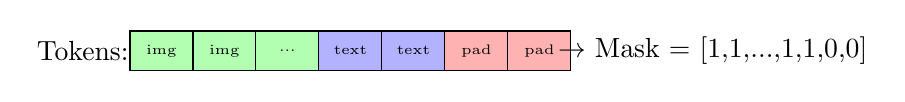
\begin{tikzpicture}[
        cell/.style={rectangle, draw, minimum width=0.8cm, minimum height=0.5cm, align=center, font=\tiny}
    ]
        \node[cell, fill=green!30] at (0,0) {img};
        \node[cell, fill=green!30] at (0.8,0) {img};
        \node[cell, fill=green!30] at (1.6,0) {...};
        \node[cell, fill=blue!30] at (2.4,0) {text};
        \node[cell, fill=blue!30] at (3.2,0) {text};
        \node[cell, fill=red!30] at (4.0,0) {pad};
        \node[cell, fill=red!30] at (4.8,0) {pad};

        \node at (-1,0) {Tokens:};
        \node at (7,0) {$\rightarrow$ Mask = [1,1,...,1,1,0,0]};
    \end{tikzpicture}
    \end{center}

    \vspace{0.5cm}
    \textbf{Implementation:}
    \begin{lstlisting}[language=Python]
# Attention mask from processor
attn_mask = inputs["attention_mask"]  # [B, seq_len]

# Expand for cross-attention
# RDT action tokens attend to all valid VLM tokens
    \end{lstlisting}
\end{frame}

%------------------------------------------------------------------------------
\begin{frame}[fragile]{RDT Forward Pass}
    \textbf{Single denoising step:}

    \vspace{0.2cm}
    \begin{lstlisting}[language=Python]
def forward(self, gt_action, states, img_cond, ...):
    t = self.sample_timesteps(batch_size)

    # Create noisy actions (flow matching)
    noise = torch.randn_like(gt_action)
    noisy_action = (1 - t) * noise + t * gt_action

    # Predict velocity
    pred_v = self.model(noisy_action, t, img_cond, ...)

    # Compute loss: target = gt - noise
    loss = F.mse_loss(pred_v, gt_action - noise)
    return loss
    \end{lstlisting}
\end{frame}

%------------------------------------------------------------------------------
\begin{frame}[fragile]{RDT Inference (1/2)}
    \textbf{Generate action from noise:}

    \vspace{0.3cm}
    \begin{lstlisting}[language=Python]
def predict_action(self, states, img_cond,
                   img_attn_mask):
    B = states.shape[0]

    # Initialize with noise
    action = torch.randn(B, 24, 20)

    # Euler integration (5 steps)
    dt = 1.0 / self.num_inference_timesteps
    for i in range(self.num_inference_timesteps):
        t = torch.full((B,), i * dt)
    \end{lstlisting}
\end{frame}

%------------------------------------------------------------------------------
\begin{frame}[fragile]{RDT Inference (2/2)}
    \textbf{Continue Euler integration:}

    \vspace{0.3cm}
    \begin{lstlisting}[language=Python]
        # Predict velocity
        v = self.model(action, t, img_cond,
                       img_attn_mask, states)

        # Euler step
        action = action + v * dt

    return action  # [B, 24, 20]
    \end{lstlisting}

    \vspace{0.5cm}
    \begin{block}{Key Points}
        \begin{itemize}
            \item 5 denoising steps (default)
            \item Simple Euler integration (no higher-order solver)
            \item Output: normalized action $[B, 24, 20]$
        \end{itemize}
    \end{block}
\end{frame}

%------------------------------------------------------------------------------
\begin{frame}{Complete FM Inference Pipeline}
    \begin{center}
    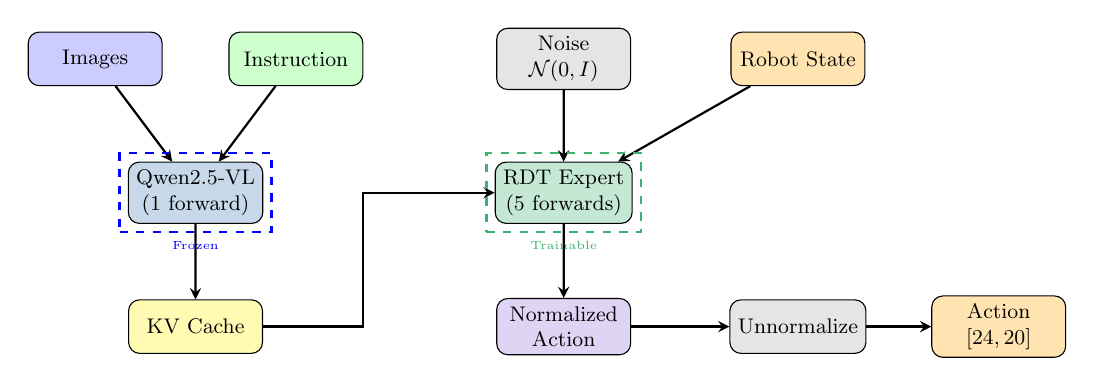
\begin{tikzpicture}[
        box/.style={rectangle, draw, rounded corners, minimum width=2cm, minimum height=0.8cm, align=center, font=\small},
        arrow/.style={->, thick, >=stealth},
        scale=0.85, transform shape
    ]
        % Row 1: Inputs (top)
        \node[box, fill=blue!20] (img) at (0,2.5) {Images};
        \node[box, fill=green!20] (inst) at (3,2.5) {Instruction};
        \node[box, fill=gray!20] (noise) at (7,2.5) {Noise\\$\mathcal{N}(0,I)$};
        \node[box, fill=actionorange!30] (state) at (10.5,2.5) {Robot State};

        % Row 2: Processing (middle)
        \node[box, fill=qwenblue!30] (qwen) at (1.5,0.5) {Qwen2.5-VL\\(1 forward)};
        \node[box, fill=rdtgreen!30] (rdt) at (7,0.5) {RDT Expert\\(5 forwards)};

        % Row 3: Intermediate (bottom-middle)
        \node[box, fill=yellow!30] (kv) at (1.5,-1.5) {KV Cache};
        \node[box, fill=vqpurple!30] (action) at (7,-1.5) {Normalized\\Action};

        % Row 4: Output (bottom)
        \node[box, fill=gray!20] (unnorm) at (10.5,-1.5) {Unnormalize};
        \node[box, fill=actionorange!30] (final) at (13.5,-1.5) {Action\\$[24,20]$};

        % Arrows - VLM path
        \draw[arrow] (img) -- (qwen);
        \draw[arrow] (inst) -- (qwen);
        \draw[arrow] (qwen) -- (kv);

        % KV Cache to RDT - horizontal then up
        \draw[arrow] (kv.east) -- ++(1.5,0) |- (rdt.west);

        % Arrows - RDT path
        \draw[arrow] (noise) -- (rdt);
        \draw[arrow] (state) -- (rdt);
        \draw[arrow] (rdt) -- (action);
        \draw[arrow] (action) -- (unnorm);
        \draw[arrow] (unnorm) -- (final);

        % Frozen indicator
        \node[draw, dashed, blue, thick, fit=(qwen), inner sep=3pt, label={[font=\tiny, blue]below:Frozen}] {};

        % Trainable indicator
        \node[draw, dashed, rdtgreen, thick, fit=(rdt), inner sep=3pt, label={[font=\tiny, rdtgreen]below:Trainable}] {};
    \end{tikzpicture}
    \end{center}
\end{frame}

%------------------------------------------------------------------------------
\begin{frame}{RDT2-FM-Post Variant}
    \begin{block}{Definition}
        RDT2-FM with additional post-training on real robot data
    \end{block}

    \vspace{0.5cm}
    \textbf{Post-Training Data:}
    \begin{itemize}
        \item UR5e manipulation demonstrations
        \item Franka FR3 manipulation demonstrations
        \item Real-world environments
    \end{itemize}

    \vspace{0.3cm}
    \textbf{Benefits:}
    \begin{itemize}
        \item Better adaptation to specific robot kinematics
        \item Improved real-world performance
        \item Reduced sim-to-real gap
    \end{itemize}

    \vspace{0.3cm}
    \begin{alertblock}{Model Location}
        \code{robotics-diffusion-transformer/RDT2-FM-Post}
    \end{alertblock}
\end{frame}

%------------------------------------------------------------------------------
\begin{frame}{Training Configuration}
    \begin{columns}[T]
        \begin{column}{0.5\textwidth}
            \textbf{RDT Expert Training:}
            \begin{table}
                \centering
                \footnotesize
                \renewcommand{\arraystretch}{1.1}
                \begin{tabular}{ll}
                    \toprule
                    \textbf{Param} & \textbf{Value} \\
                    \midrule
                    Batch size & 256 \\
                    LR & $10^{-4}$ \\
                    Max steps & 1M \\
                    Optimizer & AdamW \\
                    Precision & bf16 \\
                    \bottomrule
                \end{tabular}
            \end{table}
        \end{column}
        \begin{column}{0.5\textwidth}
            \textbf{Data Augmentation:}
            \begin{itemize}
                \item Color jitter, crop
                \item \code{cond\_mask}: 0.1
                \item \code{cam\_mask}: 0.2
            \end{itemize}
        \end{column}
    \end{columns}
\end{frame}

%------------------------------------------------------------------------------
\begin{frame}{Condition Masking}
    \begin{block}{Purpose}
        Enable classifier-free guidance and robustness
    \end{block}

    \vspace{0.3cm}
    \textbf{During Training:}
    \begin{itemize}
        \item With probability \code{cond\_mask\_prob} = 0.1:
              \begin{itemize}
                  \item Drop language instruction
                  \item Replace with null embedding
              \end{itemize}
        \item With probability \code{cam\_ext\_mask\_prob} = 0.2:
              \begin{itemize}
                  \item Mask one or both camera inputs
                  \item Replace with zeros
              \end{itemize}
    \end{itemize}

    \vspace{0.3cm}
    \textbf{During Inference:}
    \begin{itemize}
        \item Can run with or without language guidance
        \item Graceful degradation if camera fails
    \end{itemize}
\end{frame}

%------------------------------------------------------------------------------
\begin{frame}{State Noise Augmentation (1/2)}
    \textbf{Add noise to robot state during training}

    \vspace{0.5cm}
    \textbf{SNR-based Noise:}
    \[
        \vect{s}_{\text{noisy}} = \vect{s} + \boldsymbol{\eta}, \quad \boldsymbol{\eta} \sim \mathcal{N}(0, \sigma^2 I)
    \]

    where $\sigma$ is computed from SNR:
    \[
        \text{SNR (dB)} = 10 \log_{10}\left(\frac{\|\vect{s}\|^2}{\|\boldsymbol{\eta}\|^2}\right)
    \]
\end{frame}

%------------------------------------------------------------------------------
\begin{frame}{State Noise Augmentation (2/2)}
    \textbf{Default:} \code{state\_noise\_snr} = 40 dB

    \vspace{0.3cm}
    \begin{block}{Purpose}
        \begin{itemize}
            \item Robustness to sensor noise
            \item Prevent overfitting to exact states
            \item Better generalization
        \end{itemize}
    \end{block}
\end{frame}

%------------------------------------------------------------------------------
\begin{frame}[fragile]{HuggingFace Model}
    \textbf{Model:} \code{robotics-diffusion-transformer/RDT2-FM}

    \vspace{0.3cm}
    \textbf{Loading:}
    \begin{lstlisting}[language=Python]
from models.rdt_runner import RDTRunner

rdt_runner = RDTRunner.from_pretrained(
    "robotics-diffusion-transformer/RDT2-FM",
    config=model_config, dtype=torch.bfloat16
)

# Frozen VLM
vlm = Qwen2_5_VLForConditionalGeneration.from_pretrained(
    "robotics-diffusion-transformer/RDT2-VQ",
    torch_dtype=torch.bfloat16
)
vlm.requires_grad_(False)  # Freeze
    \end{lstlisting}
\end{frame}

%------------------------------------------------------------------------------
\begin{frame}[fragile]{RDTInferencer Wrapper (1/2)}
    \textbf{High-level inference interface:}

    \vspace{0.3cm}
    \begin{lstlisting}[language=Python]
from models.rdt_inferencer import RDTInferencer

model = RDTInferencer(
    config=config,
    pretrained_path="path/to/rdt_checkpoint",
    normalizer_path="path/to/normalizer.pt",
    pretrained_vision_language_model_name_or_path=
        "robotics-diffusion-transformer/RDT2-VQ",
    device="cuda:0",
    dtype=torch.bfloat16
)
    \end{lstlisting}
\end{frame}

%------------------------------------------------------------------------------
\begin{frame}[fragile]{RDTInferencer Wrapper (2/2)}
    \textbf{Usage:}
    \begin{lstlisting}[language=Python]
# Reset before each episode
model.reset()

# Single step inference
action = model.step(observations, instruction)
# Returns: [24, 20] tensor
    \end{lstlisting}

    \vspace{0.5cm}
    \begin{alertblock}{Important}
        \code{model.reset()} must be called before each new task episode
    \end{alertblock}
\end{frame}

%------------------------------------------------------------------------------
\begin{frame}[fragile]{Language Embedding Cache (1/2)}
    \begin{block}{Optimization}
        Cache VLM outputs for repeated instructions
    \end{block}

    \begin{lstlisting}[language=Python]
class RDTInferencer:
    def __init__(self, ...):
        self.lang_embeds_cache = {}  # Max 1024
    \end{lstlisting}
\end{frame}

%------------------------------------------------------------------------------
\begin{frame}[fragile]{Language Embedding Cache (2/2)}
    \begin{lstlisting}[language=Python]
def step(self, obs, instruction):
    if instruction not in self.lang_embeds_cache:
        kv_cache = self.encode(obs, instruction)
        self.lang_embeds_cache[instruction] = kv_cache
    else:
        kv_cache = self.lang_embeds_cache[instruction]
    return self.policy.predict_action(kv_cache, ...)
    \end{lstlisting}
\end{frame}

%------------------------------------------------------------------------------
\begin{frame}{Language Embedding Cache: Benefits}
    \begin{alertblock}{Key Benefits}
        \begin{itemize}
            \item Skip VLM forward for repeated instructions
            \item Reduces latency for multi-step tasks
            \item Bounded cache size (max 1024 entries)
        \end{itemize}
    \end{alertblock}
\end{frame}

%------------------------------------------------------------------------------
\begin{frame}{RDT2-FM Strengths}
    \textbf{Key Advantages:}
    \begin{itemize}
        \item Only 6 forward passes (vs 27+ for VQ)
        \item No discretization error (continuous output)
        \item Low VRAM requirement ($\sim$16GB)
        \item Fast training (frozen VLM)
    \end{itemize}
\end{frame}

%------------------------------------------------------------------------------
\begin{frame}{RDT2-FM Weaknesses}
    \textbf{Limitations:}
    \begin{itemize}
        \item Frozen VLM (no fine-tuning adaptation)
        \item Still requires 5 RDT passes
        \item Normalizer dependency for action scaling
        \item Separate models to manage
    \end{itemize}
\end{frame}

%------------------------------------------------------------------------------
\begin{frame}{RDT2-FM: Latency \& Use Cases}
    \begin{alertblock}{Latency Analysis}
        1 VLM ($\sim$50ms) + 5 RDT ($\sim$15ms each) = $\sim$125ms \\
        $\sim$3$\times$ faster than RDT2-VQ
    \end{alertblock}

    \vspace{0.3cm}
    \begin{block}{When to Use RDT2-FM}
        \begin{itemize}
            \item Real-time control requirements
            \item Limited GPU memory (16GB)
        \end{itemize}
    \end{block}
\end{frame}

%------------------------------------------------------------------------------
\begin{frame}{RDT2-FM Summary (1/2)}
    \begin{table}
        \centering
        \renewcommand{\arraystretch}{1.3}
        \begin{tabular}{ll}
            \toprule
            \textbf{Attribute} & \textbf{Value} \\
            \midrule
            VLM Backbone & Qwen2.5-VL-7B (frozen) \\
            Action Expert & 400M RDT transformer \\
            Output type & Continuous \\
            Denoising steps & 5 \\
            Total forward passes & 6 \\
            \bottomrule
        \end{tabular}
    \end{table}
\end{frame}

%------------------------------------------------------------------------------
\begin{frame}{RDT2-FM Summary (2/2)}
    \begin{table}
        \centering
        \renewcommand{\arraystretch}{1.3}
        \begin{tabular}{ll}
            \toprule
            \textbf{Attribute} & \textbf{Value} \\
            \midrule
            Action chunk & 24 frames (0.8s) \\
            Inference time & $\sim$125ms \\
            Training VRAM & $\sim$16 GB \\
            \bottomrule
        \end{tabular}
    \end{table}

    \vspace{0.3cm}
    \begin{block}{Use Case}
        Best for real-time applications where latency matters and VLM adaptation is not critical
    \end{block}
\end{frame}


% %==============================================================================
% PART 6: TRAINING PIPELINE
%==============================================================================

\section{Training Pipeline}

%------------------------------------------------------------------------------
\begin{frame}{Three-Stage Training}
    \begin{center}
    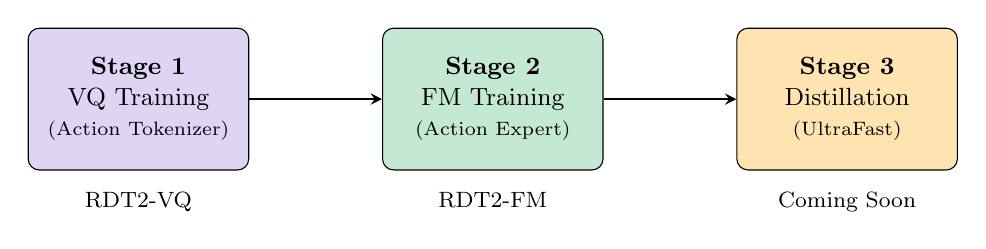
\begin{tikzpicture}[
        stage/.style={rectangle, draw, rounded corners, minimum width=2.8cm, minimum height=1.8cm, align=center, font=\small},
        arrow/.style={->, thick, >=stealth}
    ]
        \node[stage, fill=vqpurple!30] (s1) at (0,0) {\textbf{Stage 1}\\VQ Training\\{\scriptsize (Action Tokenizer)}};
        \node[stage, fill=rdtgreen!30] (s2) at (4.5,0) {\textbf{Stage 2}\\FM Training\\{\scriptsize (Action Expert)}};
        \node[stage, fill=actionorange!30] (s3) at (9,0) {\textbf{Stage 3}\\Distillation\\{\scriptsize (UltraFast)}};

        \draw[arrow] (s1) -- (s2);
        \draw[arrow] (s2) -- (s3);

        \node[below=0.15cm, font=\footnotesize] at (s1.south) {RDT2-VQ};
        \node[below=0.15cm, font=\footnotesize] at (s2.south) {RDT2-FM};
        \node[below=0.15cm, font=\footnotesize] at (s3.south) {Coming Soon};
    \end{tikzpicture}
    \end{center}

    \vspace{0.5cm}
    \textbf{Stage 1:} Train VLA with VQVAE action tokenizer \\
    \textbf{Stage 2:} Train RDT action expert with frozen VLM \\
    \textbf{Stage 3:} Distill to single-step model (future)
\end{frame}

%------------------------------------------------------------------------------
\begin{frame}{Training Entry Points}
    \textbf{Key Files:}

    \vspace{0.5cm}
    \begin{table}
        \centering
        \renewcommand{\arraystretch}{1.3}
        \begin{tabular}{lll}
            \toprule
            \textbf{Stage} & \textbf{Entry Point} & \textbf{Purpose} \\
            \midrule
            Stage 1 (VQ) & \code{main.py} & VLA fine-tuning \\
            Stage 1 (VQ) & \code{train.py} & Core training loop \\
            Stage 2 (FM) & \code{rdt/main.py} & RDT training entry \\
            Stage 2 (FM) & \code{rdt/train.py} & RDT training loop \\
            \bottomrule
        \end{tabular}
    \end{table}

    \vspace{0.5cm}
    \textbf{Training Scripts:}
    \begin{itemize}
        \item \code{scripts/finetune\_lora.sh} - LoRA ($\sim$32GB)
        \item \code{scripts/finetune\_full\_param.sh} - Full ($\sim$80GB)
        \item \code{scripts/finetune\_rdt.sh} - RDT only ($\sim$16GB)
    \end{itemize}
\end{frame}

%------------------------------------------------------------------------------
\begin{frame}{Stage 1: VLA Training Overview}
    \begin{center}
    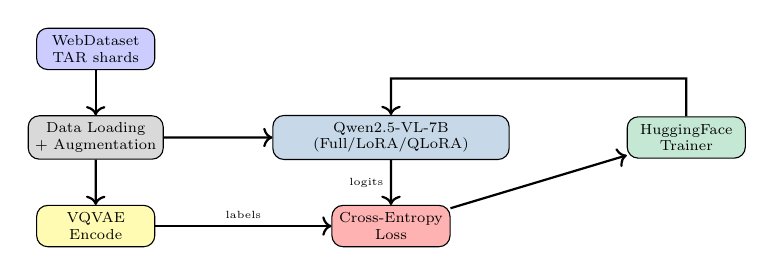
\begin{tikzpicture}[
        box/.style={rectangle, draw, rounded corners, minimum width=2cm, minimum height=0.7cm, align=center, font=\scriptsize},
        arrow/.style={->, thick},
        scale=0.75, transform shape
    ]
        % Data
        \node[box, fill=blue!20] (data) at (0,3) {WebDataset\\TAR shards};

        % Processing
        \node[box, fill=gray!30] (load) at (0,1.5) {Data Loading\\+ Augmentation};
        \node[box, fill=yellow!30] (vae) at (0,0) {VQVAE\\Encode};

        % Model
        \node[box, fill=qwenblue!30, minimum width=4cm] (qwen) at (5,1.5) {Qwen2.5-VL-7B\\(Full/LoRA/QLoRA)};

        % Loss
        \node[box, fill=red!30] (loss) at (5,0) {Cross-Entropy\\Loss};

        % Trainer
        \node[box, fill=rdtgreen!30] (trainer) at (10,1.5) {HuggingFace\\Trainer};

        % Arrows
        \draw[arrow] (data) -- (load);
        \draw[arrow] (load) -- (vae);
        \draw[arrow] (load) -- (qwen);
        \draw[arrow] (vae) -- node[above, font=\tiny] {labels} (loss);
        \draw[arrow] (qwen) -- node[left, font=\tiny] {logits} (loss);
        \draw[arrow] (loss) -- (trainer);
        \draw[arrow] (trainer) -- ++(0,1) -| (qwen);
    \end{tikzpicture}
    \end{center}
\end{frame}

%------------------------------------------------------------------------------
\begin{frame}[fragile]{main.py: Command-Line Arguments}
    \begin{columns}[T]
        \begin{column}{0.5\textwidth}
            \textbf{Model:}
            \begin{lstlisting}[language=Python]
--pretrained_model_name_or_path
--vae_name
--output_dir
            \end{lstlisting}

            \textbf{Training:}
            \begin{lstlisting}[language=Python]
--train_batch_size 4
--learning_rate 5e-6
--lr_warmup_steps 500
            \end{lstlisting}
        \end{column}
        \begin{column}{0.5\textwidth}
            \textbf{LoRA:}
            \begin{lstlisting}[language=Python]
--use_lora False
--use_qlora False
--lora_r 8
--lora_alpha 8
--lora_dropout 0.1
            \end{lstlisting}
        \end{column}
    \end{columns}
\end{frame}

%------------------------------------------------------------------------------
\begin{frame}[fragile]{train.py: Core Training Loop}
    \textbf{1. Model Loading:}
    \begin{lstlisting}[language=Python]
# Load Vision-Language Model
model = Qwen2_5_VLForConditionalGeneration \
    .from_pretrained(
        args.pretrained_model_name_or_path,
        torch_dtype=weight_dtype,
        attn_implementation="flash_attention_2"
    )

# Load Action Tokenizer
vae = MultiVQVAE.from_pretrained(args.vae_name)
vae = vae.to("cuda").float()
    \end{lstlisting}

    \vspace{0.3cm}
    \textbf{2. LoRA Setup (if enabled):}
    \begin{lstlisting}[language=Python]
if args.use_lora:
    model = get_peft_model(model, lora_config)
    model.print_trainable_parameters()
    \end{lstlisting}
\end{frame}

%------------------------------------------------------------------------------
\begin{frame}[fragile]{Collate Function (1/2)}
    \textbf{Prepare batch for training:}

    \vspace{0.3cm}
    \begin{lstlisting}[language=Python]
def collate_fn(examples):
    # 1. Process images
    images = [preprocess_image(ex["image"]) for ex in examples]

    # 2. Encode actions to tokens
    actions = torch.stack([ex["action"] for ex in examples])
    action_tokens = vae.encode(actions)  # [B, 27]

    # 3. Convert to VLA token IDs
    vla_tokens = vocab_size - action_tokens - 1
    \end{lstlisting}
\end{frame}

%------------------------------------------------------------------------------
\begin{frame}[fragile]{Collate Function (2/2)}
    \textbf{Continue batch preparation:}

    \vspace{0.3cm}
    \begin{lstlisting}[language=Python]
    # 4. Build chat template
    messages = build_chat_messages(images, instructions)
    inputs = processor(messages)

    # 5. Insert action tokens into labels
    labels = inputs["input_ids"].clone()
    labels[~action_mask] = -100  # Ignore non-action

    return {"input_ids": ..., "labels": labels, ...}
    \end{lstlisting}

    \vspace{0.3cm}
    \begin{block}{Key Points}
        \begin{itemize}
            \item VQVAE encodes actions to 27 discrete tokens
            \item Only action tokens contribute to loss (label mask)
        \end{itemize}
    \end{block}
\end{frame}

%------------------------------------------------------------------------------
\begin{frame}[fragile]{Training Arguments}
    \begin{lstlisting}[language=Python]
TrainingArguments(
    output_dir=args.output_dir,
    per_device_train_batch_size=args.train_batch_size,
    per_device_eval_batch_size=args.eval_batch_size,
    learning_rate=args.learning_rate,
    max_steps=args.max_train_steps,
    bf16=True,  # Mixed precision
    deepspeed=args.deepspeed,  # DeepSpeed config
    gradient_checkpointing=args.gradient_checkpointing,
    gradient_accumulation_steps=
        args.gradient_accumulation_steps,
    save_steps=args.checkpointing_steps,
    save_total_limit=args.checkpoints_total_limit,
    logging_steps=10,
    dataloader_num_workers=16,
    dataloader_pin_memory=True,
)
    \end{lstlisting}
\end{frame}

%------------------------------------------------------------------------------
\begin{frame}[fragile]{DeepSpeed ZeRO-1 Configuration}
    \textbf{File:} \code{scripts/zero1.json}

    \vspace{0.3cm}
    \begin{lstlisting}[language=Python]
{
    "bf16": {"enabled": "auto"},
    "train_micro_batch_size_per_gpu": "auto",
    "train_batch_size": "auto",
    "gradient_accumulation_steps": "auto",
    "zero_optimization": {
        "stage": 1,
        "allgather_partitions": true,
        "allgather_bucket_size": 5e8,
        "overlap_comm": true,
        "contiguous_gradients": true,
        "reduce_bucket_size": 8e8
    },
    "gradient_clipping": "auto"
}
    \end{lstlisting}

    \vspace{0.3cm}
    \textbf{ZeRO Stage 1:} Optimizer state partitioning only
\end{frame}

%------------------------------------------------------------------------------
\begin{frame}[fragile]{VLATrainer: Custom Evaluation}
    \begin{columns}[T]
        \begin{column}{0.55\textwidth}
            \textbf{File:} \code{vla\_trainer.py}
            \begin{lstlisting}[language=Python]
class VLATrainer(Trainer):
    def __init__(self, num_eval_datasets=2,
                 num_eval_batches=4, **kwargs):
        super().__init__(**kwargs)
        ...

    def evaluation_loop(self, ...):
        # Custom metrics computation
        ...
            \end{lstlisting}
        \end{column}
        \begin{column}{0.45\textwidth}
            \textbf{Features:}
            \begin{itemize}
                \item Multi-dataset eval
                \item Limited batch eval
                \item Custom metrics:
                \begin{itemize}
                    \item valid\_rate
                    \item mse\_error
                    \item geodesic
                \end{itemize}
            \end{itemize}
        \end{column}
    \end{columns}
\end{frame}

%------------------------------------------------------------------------------
\begin{frame}[fragile]{Evaluation Metrics Computation}
    \begin{lstlisting}[language=Python]
def compute_action_metrics(pred_action, gt_action):
    # 1. Valid rate
    valid_mask = (pred_tokens >= 0) & (pred_tokens < 1024)
    valid_rate = valid_mask.float().mean()

    # 2. MSE (total)
    mse_error = F.mse_loss(pred_action, gt_action)

    # 3. MSE (position) - indices [0:3, 10:13]
    mse_pos = F.mse_loss(pred_action[..., pos_idx],
                         gt_action[..., pos_idx])

    # 4. Geodesic (rotation) - indices [3:9, 13:19]
    R_pred = rot6d_to_matrix(pred_action[..., rot_idx])
    R_gt = rot6d_to_matrix(gt_action[..., rot_idx])
    geodesic = compute_geodesic_distance(R_pred, R_gt)

    # 5. MSE (gripper) - indices [9, 19]
    mse_grip = F.mse_loss(pred_action[..., grip_idx],
                          gt_action[..., grip_idx])
    \end{lstlisting}
\end{frame}

%------------------------------------------------------------------------------
\begin{frame}{Stage 2: RDT Training Overview}
    \begin{center}
    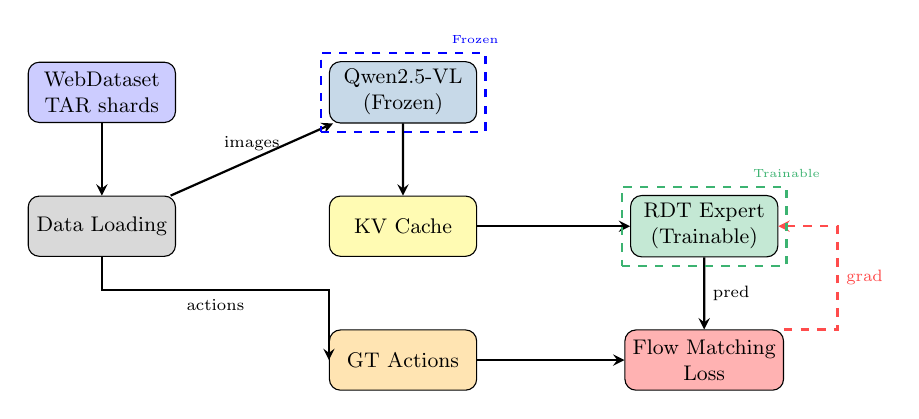
\begin{tikzpicture}[
        box/.style={rectangle, draw, rounded corners, minimum width=2.2cm, minimum height=0.9cm, align=center, font=\small},
        arrow/.style={->, thick, >=stealth},
        scale=0.85, transform shape
    ]
        % Row 1: Data source
        \node[box, fill=blue!20] (data) at (0,3) {WebDataset\\TAR shards};

        % Row 2: Data loading and VLM
        \node[box, fill=gray!30] (load) at (0,1) {Data Loading};
        \node[box, fill=qwenblue!30] (qwen) at (4.5,3) {Qwen2.5-VL\\(Frozen)};
        \node[box, fill=yellow!30] (kv) at (4.5,1) {KV Cache};

        % Row 3: RDT Expert
        \node[box, fill=rdtgreen!30] (rdt) at (9,1) {RDT Expert\\(Trainable)};

        % Row 4: Loss
        \node[box, fill=red!30] (loss) at (9,-1) {Flow Matching\\Loss};

        % Ground truth actions
        \node[box, fill=actionorange!30] (gt) at (4.5,-1) {GT Actions};

        % Arrows - Data flow
        \draw[arrow] (data) -- (load);
        \draw[arrow] (load) -- node[above, font=\scriptsize] {images} (qwen);
        \draw[arrow] (qwen) -- (kv);
        \draw[arrow] (kv) -- (rdt);

        % Actions arrow - goes below to avoid collision
        \draw[arrow] (load.south) -- ++(0,-0.5) -| node[below, font=\scriptsize, pos=0.25] {actions} (gt.west);
        \draw[arrow] (gt) -- (loss);

        % RDT to Loss
        \draw[arrow] (rdt) -- node[right, font=\scriptsize] {pred} (loss);

        % Gradient flow (backprop) - dashed
        \draw[arrow, dashed, red!70] (loss.north east) -- ++(0.8,0) |- node[right, font=\scriptsize, pos=0.25] {grad} (rdt.east);

        % Frozen indicator
        \node[draw, dashed, blue, thick, fit=(qwen), inner sep=3pt, label={[font=\tiny, blue]above right:Frozen}] {};

        % Trainable indicator
        \node[draw, dashed, rdtgreen, thick, fit=(rdt), inner sep=3pt, label={[font=\tiny, rdtgreen]above right:Trainable}] {};
    \end{tikzpicture}
    \end{center}
\end{frame}

%------------------------------------------------------------------------------
\begin{frame}[fragile]{rdt/main.py: Arguments}
    \begin{columns}[T]
        \begin{column}{0.5\textwidth}
            \textbf{Model:}
            \begin{lstlisting}[language=Python]
--config_path
--pretrained_vlm_path
--webdataset_config
            \end{lstlisting}

            \textbf{Training:}
            \begin{lstlisting}[language=Python]
--train_batch_size 256
--max_train_steps 1M
--learning_rate 1e-4
            \end{lstlisting}
        \end{column}
        \begin{column}{0.5\textwidth}
            \textbf{Augmentation:}
            \begin{lstlisting}[language=Python]
--image_aug False
--cond_mask_prob 0.1
--cam_ext_mask_prob 0.2
--state_noise_snr 40
            \end{lstlisting}
        \end{column}
    \end{columns}
\end{frame}

%------------------------------------------------------------------------------
\begin{frame}[fragile]{rdt/train.py: Training Loop}
    \begin{lstlisting}[language=Python]
for step in range(args.max_train_steps):
    batch = next(train_dataloader)

    # 1. Normalize actions
    naction = normalizer["action"].normalize(batch["actions"])

    # 2. Extract VLM features (frozen)
    with torch.no_grad():
        kv_cache = extract_kv_cache(vlm, batch)

    # 3. RDT forward (flow-matching loss)
    loss = rdt_runner(naction, batch["states"], kv_cache, ...)

    # 4. Backward + optimize
    accelerator.backward(loss)
    optimizer.step(); lr_scheduler.step(); optimizer.zero_grad()
    \end{lstlisting}
\end{frame}

%------------------------------------------------------------------------------
\begin{frame}[fragile]{Dataset Configuration (1/2)}
    \textbf{File:} \code{configs/datasets/example.yaml}

    \vspace{0.3cm}
    \textbf{Single Dataset:}
    \begin{lstlisting}[language=Python]
name: bimanual/ur_example
type: single
shards_dir: /path/to/shards
kwargs:
  instruction_path: /path/to/instruction.json
  normalizer_path: /path/to/normalizer.pt
    \end{lstlisting}
\end{frame}

%------------------------------------------------------------------------------
\begin{frame}[fragile]{Dataset Configuration (2/2)}
    \textbf{Blended Dataset:}
    \begin{lstlisting}[language=Python]
name: blended_dataset
type: blended
datasets:
  - name: dataset1
    weight: 0.5
    config_path: configs/datasets/dataset1.yaml
  - name: dataset2
    weight: 0.5
    config_path: configs/datasets/dataset2.yaml
    \end{lstlisting}

    \vspace{0.5cm}
    \begin{block}{Dataset Blending}
        Multiple datasets can be combined with different weights for diverse training data
    \end{block}
\end{frame}

%------------------------------------------------------------------------------
\begin{frame}[fragile]{WebDataset Loading (1/2)}
    \textbf{File:} \code{rdt/dataset.py}

    \vspace{0.3cm}
    \begin{lstlisting}[language=Python]
def get_train_dataset(shards_dir):
    # Load TAR shards
    dataset = wds.WebDataset(shards_dir)
    dataset = dataset.shuffle(1000)
    dataset = dataset.decode("pil")

    # Map to dictionary
    dataset = dataset.map(lambda x: {
        "image": x["image.jpg"],
        "action": np.load(io.BytesIO(x["action.npy"])),
        "meta": json.loads(x["meta.json"])
    })
    return dataset
    \end{lstlisting}
\end{frame}

%------------------------------------------------------------------------------
\begin{frame}[fragile]{WebDataset Loading (2/2)}
    \textbf{Multi-Dataset Blending:}
    \begin{lstlisting}[language=Python]
dataset = wds.RandomMix(datasets, weights)
    \end{lstlisting}

    \vspace{0.5cm}
    \begin{block}{WebDataset Benefits}
        \begin{itemize}
            \item Streaming from TAR archives (no extraction)
            \item Built-in shuffling and parallel loading
            \item Supports distributed training
        \end{itemize}
    \end{block}
\end{frame}

%------------------------------------------------------------------------------
\begin{frame}[fragile]{Normalizer (1/2)}
    \textbf{File:} \code{models/normalizer/normalizer.py}

    \vspace{0.3cm}
    \textbf{Normalization Modes:}
    \begin{itemize}
        \item \code{"limits"}: Min-max $\rightarrow [-1, 1]$
        \item \code{"gaussian"}: Standardization $\rightarrow \mu=0, \sigma=1$
    \end{itemize}

    \vspace{0.3cm}
    \begin{lstlisting}[language=Python]
# Forward normalization
x_norm = x * scale + offset

# Inverse normalization
x_orig = (x - offset) / scale
    \end{lstlisting}
\end{frame}

%------------------------------------------------------------------------------
\begin{frame}[fragile]{Normalizer (2/2)}
    \begin{lstlisting}[language=Python]
# Field-specific access
normalizer["action"].normalize(action)
normalizer["action"].unnormalize(action)

# Save/Load
normalizer.save("normalizer.pt")
normalizer = LinearNormalizer.load("normalizer.pt")
    \end{lstlisting}
\end{frame}

%------------------------------------------------------------------------------
\begin{frame}[fragile]{Training Script: LoRA}
    \textbf{File:} \code{scripts/finetune\_lora.sh}

    \vspace{0.3cm}
    \begin{lstlisting}[language=bash]
accelerate launch --config_file scripts/zero1.json main.py \
    --pretrained_model_name_or_path \
        robotics-diffusion-transformer/RDT2-VQ \
    --vae_name \
        robotics-diffusion-transformer/RVQActionTokenizer \
    --dataset configs/datasets/your_dataset.yaml \
    --output_dir outputs/lora_finetune \
    --train_batch_size 96 \
    --max_train_steps 10000 \
    --learning_rate 1e-4 \
    --lr_scheduler cosine \
    --mixed_precision bf16 \
    --use_lora \
    --gradient_checkpointing \
    --checkpointing_steps 1000 \
    --dataloader_num_workers 16
    \end{lstlisting}

    \vspace{0.3cm}
    \textbf{VRAM:} $\sim$32 GB
\end{frame}

%------------------------------------------------------------------------------
\begin{frame}[fragile]{Training Script: Full Parameter}
    \textbf{File:} \code{scripts/finetune\_full\_param.sh}

    \vspace{0.3cm}
    \begin{lstlisting}[language=bash]
accelerate launch --config_file scripts/zero1.json main.py \
    --pretrained_model_name_or_path \
        robotics-diffusion-transformer/RDT2-VQ \
    --vae_name \
        robotics-diffusion-transformer/RVQActionTokenizer \
    --dataset configs/datasets/your_dataset.yaml \
    --output_dir outputs/full_finetune \
    --train_batch_size 64 \
    --max_train_steps 10000 \
    --learning_rate 1e-5 \
    --lr_scheduler cosine \
    --mixed_precision bf16 \
    --gradient_checkpointing \
    --checkpointing_steps 1000 \
    --dataloader_num_workers 16
    \end{lstlisting}

    \vspace{0.3cm}
    \textbf{VRAM:} $\sim$80 GB (A100 80GB / H100)
\end{frame}

%------------------------------------------------------------------------------
\begin{frame}[fragile]{Training Script: RDT Only}
    \textbf{File:} \code{scripts/finetune\_rdt.sh}

    \vspace{0.3cm}
    \begin{lstlisting}[language=bash]
accelerate launch --config_file scripts/zero1.json \
    rdt/main.py \
    --pretrained_vision_language_model_name_or_path \
        robotics-diffusion-transformer/RDT2-VQ \
    --config_path configs/rdt/post_train.yaml \
    --webdataset_config configs/datasets/your_dataset.yaml \
    --output_dir outputs/rdt_finetune \
    --train_batch_size 64 \
    --sample_batch_size 32 \
    --max_train_steps 1000000 \
    --learning_rate 1e-4 \
    --checkpointing_period 5000 \
    --sample_period 1000 \
    --image_aug
    \end{lstlisting}

    \vspace{0.3cm}
    \textbf{VRAM:} $\sim$16 GB (RTX 4090)
\end{frame}

%------------------------------------------------------------------------------
\begin{frame}{VRAM Requirements Summary}
    \begin{table}
        \centering
        \renewcommand{\arraystretch}{1.4}
        \begin{tabular}{lccc}
            \toprule
            \textbf{Training Mode} & \textbf{VRAM} & \textbf{GPU Example} & \textbf{Params} \\
            \midrule
            Full Fine-tune & $\geq$80 GB & A100 80GB / H100 & 7B \\
            LoRA & $\geq$32 GB & A100 40GB & $\sim$20M \\
            QLoRA & $\geq$20 GB & RTX 4090 & $\sim$20M \\
            RDT Only & $\sim$16 GB & RTX 4090 & 400M \\
            Inference & $\sim$16 GB & RTX 4090 & -- \\
            \bottomrule
        \end{tabular}
    \end{table}

    \vspace{0.5cm}
    \begin{alertblock}{Recommendation}
        For most use cases, \textbf{RDT-only training} ($\sim$16GB) provides good results with minimal hardware requirements
    \end{alertblock}
\end{frame}

%------------------------------------------------------------------------------
\begin{frame}{Training Tips}
    \textbf{1. Learning Rate:}
    \begin{itemize}
        \item Full fine-tune: $1 \times 10^{-5}$
        \item LoRA: $1 \times 10^{-4}$
        \item RDT: $1 \times 10^{-4}$
    \end{itemize}

    \vspace{0.3cm}
    \textbf{2. Batch Size:}
    \begin{itemize}
        \item Larger is better for RDT (256+ recommended)
        \item Use gradient accumulation if limited VRAM
    \end{itemize}

    \vspace{0.3cm}
    \textbf{3. Gradient Checkpointing:}
    \begin{itemize}
        \item Enable for large models (\code{--gradient\_checkpointing})
        \item Trades compute for memory
    \end{itemize}

    \vspace{0.3cm}
    \textbf{4. Mixed Precision:}
    \begin{itemize}
        \item Always use \code{bf16} on modern GPUs
        \item Better numerical stability than \code{fp16}
    \end{itemize}
\end{frame}

%------------------------------------------------------------------------------
\begin{frame}[fragile]{Checkpointing}
    \textbf{Checkpoint Contents:}

    \vspace{0.3cm}
    \begin{itemize}
        \item \code{model.safetensors} - Model weights
        \item \code{optimizer.pt} - Optimizer state
        \item \code{scheduler.pt} - LR scheduler state
        \item \code{trainer\_state.json} - Training metadata
        \item \code{config.json} - Model configuration
    \end{itemize}

    \vspace{0.5cm}
    \textbf{Checkpoint Management:}
    \begin{lstlisting}[language=Python]
--checkpointing_steps 1000      # Save every N steps
--checkpoints_total_limit 20    # Keep last N checkpoints
    \end{lstlisting}

    \vspace{0.3cm}
    \textbf{Resume Training:}
    \begin{lstlisting}[language=Python]
--resume_from_checkpoint path/to/checkpoint
    \end{lstlisting}
\end{frame}

%------------------------------------------------------------------------------
\begin{frame}{Training Monitoring (1/2)}
    \textbf{Logged Metrics:}

    \vspace{0.3cm}
    \begin{table}
        \centering
        \renewcommand{\arraystretch}{1.2}
        \begin{tabular}{ll}
            \toprule
            \textbf{Metric} & \textbf{Description} \\
            \midrule
            \code{train/loss} & Training loss \\
            \code{train/learning\_rate} & Current LR \\
            \code{eval/valid\_rate} & Valid token ratio \\
            \code{eval/mse\_error} & Total MSE \\
            \bottomrule
        \end{tabular}
    \end{table}
\end{frame}

%------------------------------------------------------------------------------
\begin{frame}{Training Monitoring (2/2)}
    \textbf{Additional Metrics:}
    \begin{table}
        \centering
        \renewcommand{\arraystretch}{1.2}
        \begin{tabular}{ll}
            \toprule
            \textbf{Metric} & \textbf{Description} \\
            \midrule
            \code{eval/mse\_error\_pos} & Position MSE \\
            \code{eval/geodesic\_error\_rot} & Rotation error \\
            \code{eval/mse\_error\_width} & Gripper MSE \\
            \bottomrule
        \end{tabular}
    \end{table}

    \vspace{0.3cm}
    \textbf{Visualization:}
    \begin{itemize}
        \item TensorBoard: \code{tensorboard --logdir outputs/}
        \item Weights \& Biases: \code{--report\_to wandb}
    \end{itemize}
\end{frame}

%------------------------------------------------------------------------------
\begin{frame}{Training Pipeline Summary}
    \begin{columns}[T]
        \begin{column}{0.5\textwidth}
            \textbf{Stage 1 (VQ):}
            \begin{itemize}
                \item Entry: \code{main.py}
                \item Model: Qwen2.5-VL
                \item Loss: Cross-entropy
                \item Output: Discrete tokens
                \item Fine-tune: Full/LoRA/QLoRA
            \end{itemize}
        \end{column}
        \begin{column}{0.5\textwidth}
            \textbf{Stage 2 (FM):}
            \begin{itemize}
                \item Entry: \code{rdt/main.py}
                \item Model: RDT Expert
                \item Loss: Flow matching
                \item Output: Continuous
                \item VLM: Frozen
            \end{itemize}
        \end{column}
    \end{columns}

    \vspace{0.5cm}
    \begin{block}{Key Files}
        \begin{itemize}
            \item \code{train.py}, \code{rdt/train.py} - Core training
            \item \code{vla\_trainer.py} - Custom evaluation
            \item \code{scripts/zero1.json} - DeepSpeed config
            \item \code{configs/datasets/*.yaml} - Dataset configs
        \end{itemize}
    \end{block}
\end{frame}


% %==============================================================================
% PART 7: INFERENCE PIPELINE
%==============================================================================

\section{Inference Pipeline}

%------------------------------------------------------------------------------
\begin{frame}{Inference Entry Points}
    \textbf{Real Robot Deployment:}

    \vspace{0.5cm}
    \begin{table}
        \centering
        \renewcommand{\arraystretch}{1.3}
        \begin{tabular}{lll}
            \toprule
            \textbf{Model} & \textbf{Entry Point} & \textbf{Characteristics} \\
            \midrule
            RDT2-VQ & \code{deploy/inference\_real\_vq.py} & 27 passes, discrete \\
            RDT2-FM & \code{deploy/inference\_real\_fm.py} & 6 passes, continuous \\
            \bottomrule
        \end{tabular}
    \end{table}

    \vspace{0.5cm}
    \textbf{Key Differences:}
    \begin{itemize}
        \item VQ: Full VLM forward, VQVAE decode
        \item FM: KV cache extraction + RDT denoising
    \end{itemize}
\end{frame}

%------------------------------------------------------------------------------
\begin{frame}{inference\_real\_vq.py: Arguments}
    \begin{lstlisting}[language=Python, basicstyle=\ttfamily\scriptsize]
@click.command()
@click.option("--input", required=True)          # Model path
@click.option("--vae_path", required=True)       # VQVAE path
@click.option("--data_config", required=True)    # Data config
@click.option("--robot_config", required=True)   # Robot config
@click.option("--steps_per_inference", default=24)
@click.option("--max_duration", default=2000000)
@click.option("--frequency", default=30)         # Control Hz
@click.option("--instruction", default=None)
@click.option("--binarize_gripper", default=False)
@click.option("--interact", default=False)       # Interactive mode
@click.option("--use_vllm", default=False)       # vLLM acceleration
    \end{lstlisting}
\end{frame}

%------------------------------------------------------------------------------
\begin{frame}{inference\_real\_fm.py: Arguments}
    \begin{lstlisting}[language=Python, basicstyle=\ttfamily\scriptsize]
@click.command()
@click.option("--input", required=True)          # RDT checkpoint
@click.option("--pretrained_vision_language_model_name_or_path",
              required=True)                     # Frozen VLM
@click.option("--normalizer_path", required=True)
@click.option("--model_config", required=True)   # RDT config
@click.option("--data_config", required=True)
@click.option("--robot_config", required=True)
@click.option("--steps_per_inference", default=24)
@click.option("--frequency", default=30)
@click.option("--instruction", default=None)
    \end{lstlisting}
\end{frame}

%------------------------------------------------------------------------------
\begin{frame}{Complete VQ Inference Pipeline}
    \begin{center}
    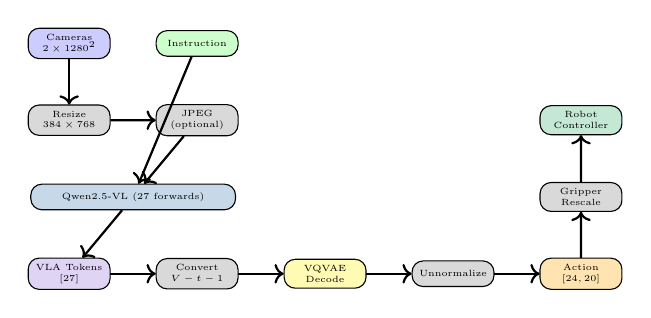
\begin{tikzpicture}[
        box/.style={rectangle, draw, rounded corners, minimum width=1.6cm, minimum height=0.5cm, align=center, font=\tiny},
        arrow/.style={->, thick},
        scale=0.65, transform shape
    ]
        % Row 1: Hardware
        \node[box, fill=blue!20] (cam) at (0,5) {Cameras\\$2 \times 1280^2$};
        \node[box, fill=green!20] (inst) at (2.5,5) {Instruction};

        % Row 2: Preprocess
        \node[box, fill=gray!30] (resize) at (0,3.5) {Resize\\$384 \times 768$};
        \node[box, fill=gray!30] (jpeg) at (2.5,3.5) {JPEG\\(optional)};

        % Row 3: Model
        \node[box, fill=qwenblue!30, minimum width=4cm] (qwen) at (1.25,2) {Qwen2.5-VL (27 forwards)};

        % Row 4: Post-process
        \node[box, fill=vqpurple!30] (tokens) at (0,0.5) {VLA Tokens\\$[27]$};
        \node[box, fill=gray!30] (convert) at (2.5,0.5) {Convert\\$V-t-1$};
        \node[box, fill=yellow!30] (vae) at (5,0.5) {VQVAE\\Decode};

        % Row 5: Action
        \node[box, fill=gray!30] (unnorm) at (7.5,0.5) {Unnormalize};
        \node[box, fill=actionorange!30] (action) at (10,0.5) {Action\\$[24,20]$};

        % Row 6: Robot
        \node[box, fill=gray!30] (grip) at (10,2) {Gripper\\Rescale};
        \node[box, fill=rdtgreen!30] (robot) at (10,3.5) {Robot\\Controller};

        % Arrows
        \draw[arrow] (cam) -- (resize);
        \draw[arrow] (resize) -- (jpeg);
        \draw[arrow] (jpeg) -- (qwen);
        \draw[arrow] (inst) -- (qwen);
        \draw[arrow] (qwen) -- (tokens);
        \draw[arrow] (tokens) -- (convert);
        \draw[arrow] (convert) -- (vae);
        \draw[arrow] (vae) -- (unnorm);
        \draw[arrow] (unnorm) -- (action);
        \draw[arrow] (action) -- (grip);
        \draw[arrow] (grip) -- (robot);
    \end{tikzpicture}
    \end{center}
\end{frame}

%------------------------------------------------------------------------------
\begin{frame}{Complete FM Inference Pipeline}
    \begin{center}
    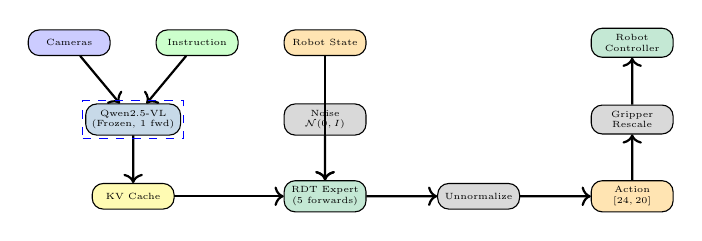
\begin{tikzpicture}[
        box/.style={rectangle, draw, rounded corners, minimum width=1.6cm, minimum height=0.5cm, align=center, font=\tiny},
        arrow/.style={->, thick},
        scale=0.65, transform shape
    ]
        % Row 1: Hardware
        \node[box, fill=blue!20] (cam) at (0,5) {Cameras};
        \node[box, fill=green!20] (inst) at (2.5,5) {Instruction};
        \node[box, fill=actionorange!30] (state) at (5,5) {Robot State};

        % Row 2: VLM
        \node[box, fill=qwenblue!30] (qwen) at (1.25,3.5) {Qwen2.5-VL\\(Frozen, 1 fwd)};
        \node[box, fill=yellow!30] (kv) at (1.25,2) {KV Cache};

        % Row 3: RDT
        \node[box, fill=gray!30] (noise) at (5,3.5) {Noise\\$\mathcal{N}(0,I)$};
        \node[box, fill=rdtgreen!30] (rdt) at (5,2) {RDT Expert\\(5 forwards)};

        % Row 4: Output
        \node[box, fill=gray!30] (unnorm) at (8,2) {Unnormalize};
        \node[box, fill=actionorange!30] (action) at (11,2) {Action\\$[24,20]$};

        % Row 5: Robot
        \node[box, fill=gray!30] (grip) at (11,3.5) {Gripper\\Rescale};
        \node[box, fill=rdtgreen!30] (robot) at (11,5) {Robot\\Controller};

        % Arrows
        \draw[arrow] (cam) -- (qwen);
        \draw[arrow] (inst) -- (qwen);
        \draw[arrow] (qwen) -- (kv);
        \draw[arrow] (kv) -- (rdt);
        \draw[arrow] (state) -- (rdt);
        \draw[arrow] (noise) -- (rdt);
        \draw[arrow] (rdt) -- (unnorm);
        \draw[arrow] (unnorm) -- (action);
        \draw[arrow] (action) -- (grip);
        \draw[arrow] (grip) -- (robot);

        % Frozen
        \node[draw, dashed, blue, fit=(qwen), inner sep=1pt] {};
    \end{tikzpicture}
    \end{center}
\end{frame}

%------------------------------------------------------------------------------
\begin{frame}{Model Loading (VQ)}
    \begin{lstlisting}[language=Python, basicstyle=\ttfamily\small]
# Load processor
processor = AutoProcessor.from_pretrained(
    "Qwen/Qwen2.5-VL-7B-Instruct")

# Load model
model = Qwen2_5_VLForConditionalGeneration \
    .from_pretrained(
        input_path,
        torch_dtype=torch.bfloat16,
        attn_implementation="flash_attention_2"
    ).to("cuda").eval()

# Load VQVAE (float32 for precision)
vae = MultiVQVAE.from_pretrained(vae_path)
vae = vae.to("cuda").float()

# Load normalizer
normalizer = LinearNormalizer.load(normalizer_path)
    \end{lstlisting}
\end{frame}

%------------------------------------------------------------------------------
\begin{frame}{Model Loading (FM)}
    \begin{lstlisting}[language=Python, basicstyle=\ttfamily\small]
from models.rdt_inferencer import RDTInferencer

model = RDTInferencer(
    config=yaml.safe_load(open(model_config)),
    pretrained_path=input_path,
    normalizer_path=normalizer_path,
    pretrained_vision_language_model_name_or_path=
        vlm_path,
    device="cuda:0",
    dtype=torch.bfloat16
)

# IMPORTANT: Reset before each episode
model.reset()
    \end{lstlisting}

    \vspace{0.3cm}
    \begin{alertblock}{Note}
        \code{model.reset()} must be called before each task episode to clear caches and compile the model
    \end{alertblock}
\end{frame}

%------------------------------------------------------------------------------
\begin{frame}{batch\_predict\_action Function}
    \textbf{File:} \code{utils.py}

    \vspace{0.3cm}
    \begin{lstlisting}[language=Python, basicstyle=\ttfamily\scriptsize]
def batch_predict_action(model, processor, vae, normalizer,
                         examples, valid_action_id_length,
                         instruction=None, apply_jpeg=False):
    # 1. Preprocess images
    images = [preprocess_data_from_umi(ex) for ex in examples]

    # 2. Build chat template
    text = processor.apply_chat_template(messages)
    text += "<|im_start|>assistant\n<|quad_start|>"

    # 3. Generate tokens
    output = model.generate(**inputs, max_new_tokens=29)

    # 4. Extract action tokens
    action_ids = extract_between_markers(output)

    # 5. Convert VLA -> VAE tokens
    vae_ids = vocab_size - (action_ids + 1)
    vae_ids = vae_ids.clamp(0, vae.num_embeddings - 1)

    # 6. Decode and unnormalize
    actions = vae.decode(vae_ids)
    actions = normalizer["action"].unnormalize(actions)
    \end{lstlisting}
\end{frame}

%------------------------------------------------------------------------------
\begin{frame}{RDTInferencer.step() Method}
    \textbf{File:} \code{models/rdt\_inferencer.py}

    \vspace{0.3cm}
    \begin{lstlisting}[language=Python, basicstyle=\ttfamily\small]
def step(self, observations, instruction):
    # 1. Extract images
    images = [observations['images'][name]
              for name in self.camera_names]

    # 2. Encode (with caching)
    if instruction not in self.lang_embeds_cache:
        kv_cache = self.encode_image_and_instruction(
            images, instruction)
        self.lang_embeds_cache[instruction] = kv_cache

    # 3. Predict action (5 denoising steps)
    action = self.policy.predict_action(
        states=observations['state'],
        img_cond=kv_cache)

    # 4. Unnormalize
    action = self.normalizer["action"].unnormalize(action)
    return action.squeeze(0)  # [24, 20]
    \end{lstlisting}
\end{frame}

%------------------------------------------------------------------------------
\begin{frame}{Latency Constants}
    \textbf{Critical timing parameters:}

    \vspace{0.5cm}
    \begin{table}
        \centering
        \renewcommand{\arraystretch}{1.4}
        \begin{tabular}{lll}
            \toprule
            \textbf{Parameter} & \textbf{Value} & \textbf{Description} \\
            \midrule
            Camera obs latency & 70 ms & Image capture delay \\
            Action execution latency & 10 ms & Command transmission \\
            Frame latency & $\sim$16.7 ms & $1/60$ second \\
            \midrule
            VQ inference & $\sim$400 ms & 27 forward passes \\
            FM inference & $\sim$125 ms & 6 forward passes \\
            \bottomrule
        \end{tabular}
    \end{table}

    \vspace{0.3cm}
    \begin{lstlisting}[language=Python, basicstyle=\ttfamily\small]
camera_obs_latency = 0.07      # 70ms
action_execution_latency = 0.01 # 10ms
frame_latency = 1/60           # ~16.7ms
    \end{lstlisting}
\end{frame}

%------------------------------------------------------------------------------
\begin{frame}{Latency Compensation}
    \begin{block}{Problem}
        By the time action executes, observation is outdated
    \end{block}

    \vspace{0.3cm}
    \textbf{Compensation Strategy:}
    \begin{enumerate}
        \item Measure inference time
        \item Calculate total latency: $L = L_{\text{obs}} + L_{\text{inf}} + L_{\text{exec}}$
        \item Skip initial actions that would be outdated
        \item Start execution from appropriate action index
    \end{enumerate}

    \vspace{0.3cm}
    \begin{lstlisting}[language=Python, basicstyle=\ttfamily\small]
# Calculate actions to skip
total_latency = camera_obs_latency + inference_time
skip_frames = int(total_latency * frequency)

# Execute remaining actions
actions_to_execute = actions[skip_frames:]
env.exec_actions(actions_to_execute,
                 compensate_latency=True)
    \end{lstlisting}
\end{frame}

%------------------------------------------------------------------------------
\begin{frame}{Gripper Rescaling}
    \begin{block}{UMI vs Real Robot}
        UMI gripper range differs from real robot gripper range
    \end{block}

    \vspace{0.5cm}
    \textbf{Rescaling Formula:}
    \[
        \boxed{g_{\text{robot}} = \frac{g_{\text{model}}}{0.088} \times 0.10}
    \]

    \vspace{0.3cm}
    \begin{itemize}
        \item UMI gripper range: $[0, 0.088]$ meters
        \item Real robot range: $[0, 0.10]$ meters
    \end{itemize}

    \vspace{0.3cm}
    \begin{lstlisting}[language=Python, basicstyle=\ttfamily\small]
# Rescale gripper for right arm (index 9)
action[:, 9] = action[:, 9] / 0.088 * 0.10

# Rescale gripper for left arm (index 19)
action[:, 19] = action[:, 19] / 0.088 * 0.10
    \end{lstlisting}
\end{frame}

%------------------------------------------------------------------------------
\begin{frame}{Binarize Gripper Option}
    \begin{block}{Purpose}
        Convert continuous gripper to binary open/close
    \end{block}

    \vspace{0.3cm}
    \textbf{Implementation:}
    \begin{lstlisting}[language=Python, basicstyle=\ttfamily\small]
if binarize_gripper:
    threshold = 0.5  # midpoint
    gripper = action[..., grip_idx]
    gripper = (gripper > threshold).float()
    action[..., grip_idx] = gripper
    \end{lstlisting}

    \vspace{0.5cm}
    \textbf{When to Use:}
    \begin{itemize}
        \item Robot gripper only supports open/close
        \item Task doesn't require precise grip width
        \item Reduces noise in gripper commands
    \end{itemize}
\end{frame}

%------------------------------------------------------------------------------
\begin{frame}{Robot Controllers}
    \textbf{Supported Robots:}

    \vspace{0.5cm}
    \begin{table}
        \centering
        \renewcommand{\arraystretch}{1.3}
        \begin{tabular}{lll}
            \toprule
            \textbf{Robot} & \textbf{Controller File} & \textbf{Protocol} \\
            \midrule
            UR5e & \code{rtde\_interpolation\_controller.py} & RTDE \\
            Franka FR3 & \code{franka\_interpolation\_controller.py} & zerorpc \\
            \bottomrule
        \end{tabular}
    \end{table}

    \vspace{0.5cm}
    \textbf{Directory:} \code{deploy/umi/real\_world/}

    \vspace{0.3cm}
    \textbf{Common Interface:}
    \begin{itemize}
        \item \code{STOP} - Halt motion
        \item \code{SERVOL} - Servo to target
        \item \code{SCHEDULE\_WAYPOINT} - Schedule future waypoint
    \end{itemize}
\end{frame}

%------------------------------------------------------------------------------
\begin{frame}{UR5e Controller (RTDE)}
    \textbf{File:} \code{rtde\_interpolation\_controller.py}

    \vspace{0.3cm}
    \begin{lstlisting}[language=Python, basicstyle=\ttfamily\small]
controller = RTDEInterpolationController(
    shm_manager=shm_manager,
    robot_ip="192.168.x.x",
    frequency=125,          # CB2=125, UR3e=500
    lookahead_time=0.1,     # [0.03, 0.2]s
    gain=300,               # [100, 2000]
    max_pos_speed=0.25,     # m/s
    max_rot_speed=0.16,     # rad/s
    tcp_offset_pose=offset,
    payload_mass=1.0,       # kg
)
    \end{lstlisting}

    \vspace{0.3cm}
    \textbf{RTDE Protocol:} Real-Time Data Exchange (125-500 Hz)
\end{frame}

%------------------------------------------------------------------------------
\begin{frame}{Franka FR3 Controller}
    \textbf{File:} \code{franka\_interpolation\_controller.py}

    \vspace{0.3cm}
    \begin{lstlisting}[language=Python, basicstyle=\ttfamily\small]
# Low-level interface
interface = FrankaInterface()
interface.go_home()
interface.get_ee_pose()
interface.get_joint_positions()
interface.start_cartesian_impedance(Kx, Kxd)
interface.update_desired_ee_pose(pose)

# High-level controller
controller = FrankaInterpolationController(
    robot_ip="localhost",
    robot_port=4243,
    frequency=1000,         # Torque control Hz
    verbose=False,
    receive_latency=latency
)
    \end{lstlisting}

    \vspace{0.3cm}
    \textbf{Communication:} zerorpc over TCP
\end{frame}

%------------------------------------------------------------------------------
\begin{frame}{BimanualUmiEnv}
    \textbf{File:} \code{deploy/umi/real\_world/bimanual\_umi\_env.py}

    \vspace{0.3cm}
    \begin{lstlisting}[language=Python, basicstyle=\ttfamily\small]
env = BimanualUmiEnv(
    output_dir=output_dir,
    cameras_config=cameras_config,
    robots_config=robots_config,
    grippers_config=grippers_config,
    frequency=20,                    # Control Hz
    max_obs_buffer_size=60,
    camera_obs_latency=0.125,
    max_pos_speed=0.25,              # m/s
    max_rot_speed=0.6,               # rad/s
)
    \end{lstlisting}

    \vspace{0.3cm}
    \textbf{Key Methods:}
    \begin{itemize}
        \item \code{get\_obs()} - Get current observation
        \item \code{exec\_actions(actions, timestamps)} - Execute actions
        \item \code{start\_episode()} / \code{end\_episode()}
    \end{itemize}
\end{frame}

%------------------------------------------------------------------------------
\begin{frame}{Observation Structure}
    \textbf{Output of \code{env.get\_obs()}:}

    \vspace{0.3cm}
    \begin{lstlisting}[language=Python, basicstyle=\ttfamily\small]
obs = {
    'camera0_rgb': np.array([H, W, 3]),  # uint8
    'camera1_rgb': np.array([H, W, 3]),  # uint8
    'robot0_eef_pos': np.array([3]),     # xyz
    'robot0_eef_rot_axis_angle': np.array([3]),
    'robot0_gripper_width': float,
    'robot1_eef_pos': np.array([3]),
    'robot1_eef_rot_axis_angle': np.array([3]),
    'robot1_gripper_width': float,
    'timestamp': float
}
    \end{lstlisting}

    \vspace{0.3cm}
    \textbf{Image Resolution:}
    \begin{itemize}
        \item Raw: $1280 \times 1024$
        \item After resize: $384 \times 384$
    \end{itemize}
\end{frame}

%------------------------------------------------------------------------------
\begin{frame}{Action Execution}
    \begin{lstlisting}[language=Python, basicstyle=\ttfamily\small]
def exec_actions(self, actions, timestamps,
                 compensate_latency=True):
    """
    Execute action sequence on robots.

    Args:
        actions: [T, 20] action chunk
        timestamps: [T] execution times
        compensate_latency: skip outdated actions

    Action dimensions per robot (10):
        [0:3] - Position (x, y, z)
        [3:9] - Rotation (6D representation)
        [9]   - Gripper width
    """
    for robot_idx in range(self.num_robots):
        robot_actions = actions[:, robot_idx*10:(robot_idx+1)*10]
        self.robots[robot_idx].schedule_waypoints(
            robot_actions, timestamps)
    \end{lstlisting}
\end{frame}

%------------------------------------------------------------------------------
\begin{frame}{Control Loop Structure}
    \begin{lstlisting}[language=Python, basicstyle=\ttfamily\scriptsize]
# Main inference loop
while True:
    # 1. Get observation
    obs = env.get_obs()
    t_obs = time.time()

    # 2. Preprocess
    data = preprocess_data_from_umi(obs, instruction)

    # 3. Predict actions
    t_start = time.time()
    actions = model.step(data, instruction)  # [24, 20]
    inference_time = time.time() - t_start

    # 4. Gripper rescaling
    actions[:, 9] = actions[:, 9] / 0.088 * 0.10
    actions[:, 19] = actions[:, 19] / 0.088 * 0.10

    # 5. Execute with latency compensation
    timestamps = compute_action_timestamps(
        t_obs, inference_time, frequency)
    env.exec_actions(actions, timestamps,
                     compensate_latency=True)
    \end{lstlisting}
\end{frame}

%------------------------------------------------------------------------------
\begin{frame}{Action Space Conversion}
    \textbf{File:} \code{deploy/umi/real\_world/real\_inference\_util.py}

    \vspace{0.3cm}
    \textbf{Policy $\rightarrow$ Robot Conversion:}
    \begin{lstlisting}[language=Python, basicstyle=\ttfamily\small]
def get_real_umi_action(action, env_obs,
                        action_pose_repr='abs'):
    """
    Convert 10-dim policy action to robot command.

    Policy (10-dim per robot):
        [0:3]  - Target EE position
        [3:9]  - Target EE rotation (6D)
        [9]    - Gripper width

    Robot command (7-dim per robot):
        [0:3]  - Position (delta or absolute)
        [3:6]  - Rotation vector (3D)
        [6]    - Gripper command
    """
    \end{lstlisting}
\end{frame}

%------------------------------------------------------------------------------
\begin{frame}{TCP Space Conversion}
    \textbf{Tracker $\rightarrow$ TCP Transformation:}

    \vspace{0.3cm}
    \begin{lstlisting}[language=Python, basicstyle=\ttfamily\small]
def convert_policy_to_tcp_space(
    action,
    T_tracker_to_policy,  # (0, 0.078, -0.026705)
    T_tracker_to_tcp,     # (0, 0.070261, 0.272602)
    backward=False
):
    """
    Transform between policy space and TCP space.

    Formula:
        T_composed = T_tracker_to_tcp^-1 @ T_tracker_to_policy
        action_tcp = composed_T @ action @ composed_T^-1
    """
    \end{lstlisting}

    \vspace{0.3cm}
    \begin{alertblock}{Important}
        This conversion is critical for accurate robot control. Incorrect TCP offset causes systematic errors.
    \end{alertblock}
\end{frame}

%------------------------------------------------------------------------------
\begin{frame}{Robot Configuration YAML}
    \textbf{File:} \code{configs/robots/eval\_bimanual\_*.yaml}

    \vspace{0.3cm}
    \begin{lstlisting}[language=Python, basicstyle=\ttfamily\scriptsize]
tx_left_right: [[4x4 transformation matrix]]
tx_tracker_to_tcp: [[4x4 transformation matrix]]

cameras:
  - serial: "camera_serial"
    fps: 30
    input_res: [1280, 1024]
    output_res: [384, 384]

robots:
  - robot_type: "franka"  # or "ur5e"
    robot_ip: "192.168.x.x"
    robot_port: 4242
    tcp_offset: 0.21
    sphere_center: [x, y, z]
    sphere_radius: 0.15

grippers:
  - gripper_ip: "192.168.x.x"
    gripper_port: 1000
    \end{lstlisting}
\end{frame}

%------------------------------------------------------------------------------
\begin{frame}{Calibration Overview}
    \textbf{Files:} \code{deploy/calibration/}

    \vspace{0.5cm}
    \textbf{Calibration Steps:}
    \begin{enumerate}
        \item \textbf{calibrate\_franka.py} - Collect tracker-robot data
              \begin{itemize}
                  \item Execute sinusoidal motion
                  \item Record tracker and robot poses
              \end{itemize}

        \item \textbf{compute\_calibration\_matrix.py} - Optimize transform
              \begin{itemize}
                  \item L-BFGS-B optimization
                  \item Minimize position + rotation error
              \end{itemize}
    \end{enumerate}

    \vspace{0.3cm}
    \textbf{Output:}
    \begin{itemize}
        \item \code{tx\_tracker\_to\_tcp}: $4 \times 4$ transformation matrix
        \item Position error: $< 5$mm typical
        \item Rotation error: $< 2^\circ$ typical
    \end{itemize}
\end{frame}

%------------------------------------------------------------------------------
\begin{frame}{vLLM Inference (VQ Only)}
    \begin{lstlisting}[language=Python, basicstyle=\ttfamily\small]
from vllm import LLM, SamplingParams

# Initialize vLLM
llm = LLM(
    model=model_path,
    dtype=torch.bfloat16,
    tensor_parallel_size=1,
    enable_chunked_prefill=True,
    gpu_memory_utilization=0.90,
    max_model_len=2048,
    limit_mm_per_prompt={"image": 1}
)

# Sampling parameters
sampling_params = SamplingParams(
    max_tokens=29,
    temperature=0.0,  # Greedy
    detokenize=False
)

# Generate
outputs = llm.generate(prompts, sampling_params)
    \end{lstlisting}
\end{frame}

%------------------------------------------------------------------------------
\begin{frame}{Interactive Mode}
    \textbf{Option:} \code{--interact}

    \vspace(0.5cm)
    \textbf{Features:}
    \begin{itemize}
        \item Change instruction during execution
        \item Keyboard control for manual override
        \item Real-time task switching
    \end{itemize}

    \vspace{0.3cm}
    \begin{lstlisting}[language=Python, basicstyle=\ttfamily\small]
if interact:
    print("Enter new instruction (or 'q' to quit):")
    user_input = input()
    if user_input == 'q':
        break
    elif user_input:
        instruction = user_input
        model.reset()  # Clear caches for new instruction
    \end{lstlisting}
\end{frame}

%------------------------------------------------------------------------------
\begin{frame}{Inference Pipeline Summary}
    \begin{table}
        \centering
        \renewcommand{\arraystretch}{1.3}
        \begin{tabular}{lcc}
            \toprule
            \textbf{Aspect} & \textbf{VQ} & \textbf{FM} \\
            \midrule
            Entry point & \code{inference\_real\_vq.py} & \code{inference\_real\_fm.py} \\
            Forward passes & 27 & 6 \\
            Inference time & $\sim$400ms & $\sim$125ms \\
            VQVAE required & Yes & No \\
            Normalizer & Yes & Yes \\
            vLLM support & Yes & No \\
            \bottomrule
        \end{tabular}
    \end{table}

    \vspace(0.5cm)
    \begin{block}{Key Steps}
        1. Load models $\rightarrow$ 2. Get observation $\rightarrow$ 3. Predict action \\
        $\rightarrow$ 4. Rescale gripper $\rightarrow$ 5. Execute with latency compensation
    \end{block}
\end{frame}


% %==============================================================================
% PART 8: DEBUGGING & MANISKILL INTEGRATION
%==============================================================================

\section{Debugging \& ManiSkill Integration}

%------------------------------------------------------------------------------
\begin{frame}{ManiSkill Integration Overview}
    \begin{block}{Challenge}
        Adapting RDT2 from real robots to ManiSkill simulation
    \end{block}

    \vspace{0.5cm}
    \textbf{Key Differences:}
    \begin{itemize}
        \item Camera configuration (fisheye vs pinhole)
        \item Action space representation
        \item Coordinate frames and conventions
        \item Control frequency and latency
    \end{itemize}

    \vspace{0.3cm}
    \begin{alertblock}{Focus Areas}
        1. Image preprocessing \\
        2. Action dimension mapping \\
        3. Normalization/Unnormalization \\
        4. Coordinate transformations
    \end{alertblock}
\end{frame}

%------------------------------------------------------------------------------
\begin{frame}{Debugging Checklist}
    \textbf{When model outputs incorrect actions:}

    \vspace{0.3cm}
    \begin{enumerate}
        \item[$\square$] \textbf{Image Format}
              \begin{itemize}
                  \item Resolution: $384 \times 384$ per camera
                  \item Concatenation: Left-Right horizontal
                  \item Color space: RGB (not BGR)
                  \item Data type: uint8 $[0, 255]$
              \end{itemize}

        \item[$\square$] \textbf{Normalization}
              \begin{itemize}
                  \item Correct normalizer file loaded
                  \item Actions normalized before encoding
                  \item Actions unnormalized after decoding
              \end{itemize}

        \item[$\square$] \textbf{Token Conversion}
              \begin{itemize}
                  \item VLA $\rightarrow$ VAE: $V - (t + 1)$
                  \item Clamping to $[0, 1023]$
              \end{itemize}
    \end{enumerate}
\end{frame}

%------------------------------------------------------------------------------
\begin{frame}{Debugging Checklist (cont.)}
    \begin{enumerate}
        \setcounter{enumi}{3}
        \item[$\square$] \textbf{Action Dimensions}
              \begin{itemize}
                  \item Position: indices [0:3, 10:13]
                  \item Rotation: indices [3:9, 13:19] (6D)
                  \item Gripper: indices [9, 19]
              \end{itemize}

        \item[$\square$] \textbf{Coordinate Frame}
              \begin{itemize}
                  \item Robot base frame vs world frame
                  \item TCP offset correctness
                  \item Left-right arm transformation
              \end{itemize}

        \item[$\square$] \textbf{Rotation Representation}
              \begin{itemize}
                  \item 6D rotation (not quaternion/euler)
                  \item Gram-Schmidt orthonormalization
                  \item Correct conversion to rotation matrix
              \end{itemize}
    \end{enumerate}
\end{frame}

%------------------------------------------------------------------------------
\begin{frame}{Common Issue: Image Format}
    \begin{block}{Symptom}
        Model outputs random/incorrect actions regardless of input
    \end{block}

    \vspace{0.3cm}
    \textbf{Correct Format:}
    \begin{lstlisting}[language=Python, basicstyle=\ttfamily\small]
# Per camera: [384, 384, 3] RGB uint8
left_img = cv2.resize(left_raw, (384, 384))
left_img = cv2.cvtColor(left_img, cv2.COLOR_BGR2RGB)

right_img = cv2.resize(right_raw, (384, 384))
right_img = cv2.cvtColor(right_img, cv2.COLOR_BGR2RGB)

# Concatenate horizontally
combined = np.concatenate([left_img, right_img], axis=1)
# Result: [384, 768, 3]
    \end{lstlisting}

    \vspace{0.3cm}
    \textbf{Common Mistakes:}
    \begin{itemize}
        \item BGR instead of RGB (OpenCV default)
        \item Wrong resize order (width vs height)
        \item Vertical instead of horizontal concatenation
    \end{itemize}
\end{frame}

%------------------------------------------------------------------------------
\begin{frame}{Common Issue: Normalizer Mismatch}
    \begin{block}{Symptom}
        Actions are scaled incorrectly (too large/small)
    \end{block}

    \vspace{0.3cm}
    \textbf{Diagnosis:}
    \begin{lstlisting}[language=Python, basicstyle=\ttfamily\small]
# Check normalizer statistics
print("Action stats:")
print(f"  Scale: {normalizer['action'].scale}")
print(f"  Offset: {normalizer['action'].offset}")
print(f"  Mode: {normalizer['action'].mode}")

# Verify range after normalization
norm_action = normalizer["action"].normalize(action)
print(f"Normalized range: [{norm_action.min()}, "
      f"{norm_action.max()}]")
# Should be roughly [-1, 1] for "limits" mode
    \end{lstlisting}

    \vspace(0.3cm)
    \textbf{Solution:}
    \begin{itemize}
        \item Use normalizer trained on same data distribution
        \item Create new normalizer from ManiSkill dataset
    \end{itemize}
\end{frame}

%------------------------------------------------------------------------------
\begin{frame}{Common Issue: Token Conversion}
    \begin{block}{Symptom}
        High invalid token rate, decoder errors
    \end{block}

    \vspace(0.3cm)
    \textbf{Correct Conversion:}
    \begin{lstlisting}[language=Python, basicstyle=\ttfamily\small]
vocab_size = 152064  # Qwen2.5-VL vocabulary

# VLA token -> VAE token
vae_token = vocab_size - (vla_token + 1)

# Clamp to valid range
vae_token = torch.clamp(vae_token, 0, 1023)

# Check valid rate
valid_mask = (vae_token >= 0) & (vae_token < 1024)
valid_rate = valid_mask.float().mean()
print(f"Valid rate: {valid_rate:.2%}")

# Should be >95% for well-trained model
    \end{lstlisting}
\end{frame}

%------------------------------------------------------------------------------
\begin{frame}{Common Issue: Rotation Format}
    \begin{block}{Symptom}
        Position correct but orientation wrong
    \end{block}

    \vspace(0.3cm)
    \textbf{6D Rotation Verification:}
    \begin{lstlisting}[language=Python, basicstyle=\ttfamily\small]
def rot6d_to_matrix(rot6d):
    """Convert 6D rotation to 3x3 matrix."""
    a1, a2 = rot6d[..., :3], rot6d[..., 3:6]

    # Gram-Schmidt orthonormalization
    b1 = F.normalize(a1, dim=-1)
    b2 = a2 - (b1 * a2).sum(-1, keepdim=True) * b1
    b2 = F.normalize(b2, dim=-1)
    b3 = torch.cross(b1, b2, dim=-1)

    return torch.stack([b1, b2, b3], dim=-2)

# Verify orthonormality
R = rot6d_to_matrix(rot6d)
I = R @ R.transpose(-1, -2)  # Should be identity
det = torch.det(R)           # Should be 1
    \end{lstlisting}
\end{frame}

%------------------------------------------------------------------------------
\begin{frame}{Common Issue: Coordinate Frame}
    \begin{block}{Symptom}
        Actions are mirrored, inverted, or offset
    \end{block}

    \vspace(0.3cm)
    \textbf{Key Transformations to Check:}

    \vspace(0.3cm)
    \begin{enumerate}
        \item \textbf{Camera-to-Robot Transform}
              \begin{itemize}
                  \item Wrist camera frame vs robot base frame
                  \item Check \code{tx\_tracker\_to\_tcp} matrix
              \end{itemize}

        \item \textbf{Left-Right Robot Transform}
              \begin{itemize}
                  \item Bimanual coordination
                  \item Check \code{tx\_left\_right} matrix
              \end{itemize}

        \item \textbf{World Frame Convention}
              \begin{itemize}
                  \item Z-up vs Y-up
                  \item Right-handed vs left-handed
              \end{itemize}
    \end{enumerate}
\end{frame}

%------------------------------------------------------------------------------
\begin{frame}{Debugging Tool: Action Visualization}
    \begin{lstlisting}[language=Python, basicstyle=\ttfamily\small]
def visualize_action_chunk(action):
    """Plot action trajectory for debugging."""
    import matplotlib.pyplot as plt

    fig, axes = plt.subplots(4, 1, figsize=(12, 10))

    # Position (right arm)
    axes[0].plot(action[:, 0:3])
    axes[0].set_title("Right Arm Position")
    axes[0].legend(['x', 'y', 'z'])

    # Rotation (right arm) - first 3 of 6D
    axes[1].plot(action[:, 3:6])
    axes[1].set_title("Right Arm Rotation (6D[:3])")

    # Gripper (right arm)
    axes[2].plot(action[:, 9])
    axes[2].set_title("Right Gripper")

    # Repeat for left arm...
    plt.tight_layout()
    plt.savefig("action_debug.png")
    \end{lstlisting}
\end{frame}

%------------------------------------------------------------------------------
\begin{frame}{Debugging Tool: Step-by-Step Trace}
    \begin{lstlisting}[language=Python, basicstyle=\ttfamily\scriptsize]
def debug_inference(model, vae, normalizer, obs, instruction):
    # 1. Image preprocessing
    img = preprocess_image(obs)
    print(f"Image shape: {img.shape}, dtype: {img.dtype}")
    print(f"Image range: [{img.min()}, {img.max()}]")

    # 2. Token generation
    tokens = model.generate(...)
    print(f"Generated tokens: {tokens.shape}")
    print(f"Token range: [{tokens.min()}, {tokens.max()}]")

    # 3. Token conversion
    vae_tokens = convert_to_vae(tokens)
    valid = (vae_tokens >= 0) & (vae_tokens < 1024)
    print(f"Valid tokens: {valid.sum()}/{len(valid)}")

    # 4. VAE decode
    action_norm = vae.decode(vae_tokens)
    print(f"Normalized action range: "
          f"[{action_norm.min():.3f}, {action_norm.max():.3f}]")

    # 5. Unnormalize
    action = normalizer["action"].unnormalize(action_norm)
    print(f"Action range: [{action.min():.3f}, {action.max():.3f}]")
    \end{lstlisting}
\end{frame}

%------------------------------------------------------------------------------
\begin{frame}{ManiSkill Adaptation: Camera Setup}
    \textbf{RDT2 expects wrist-mounted fisheye cameras:}

    \vspace(0.3cm)
    \begin{table}
        \centering
        \renewcommand{\arraystretch}{1.3}
        \begin{tabular}{lcc}
            \toprule
            \textbf{Aspect} & \textbf{RDT2 (Real)} & \textbf{ManiSkill} \\
            \midrule
            Camera type & Fisheye & Pinhole \\
            Mount & Wrist & Configurable \\
            Resolution & $384 \times 384$ & Variable \\
            FOV & Wide ($\sim$180$^\circ$) & Narrow \\
            \bottomrule
        \end{tabular}
    \end{table}

    \vspace(0.3cm)
    \textbf{Adaptation Options:}
    \begin{itemize}
        \item Mount cameras at wrist in ManiSkill
        \item Apply fisheye distortion to pinhole images
        \item Fine-tune model on ManiSkill images
    \end{itemize}
\end{frame}

%------------------------------------------------------------------------------
\begin{frame}{ManiSkill Adaptation: Action Space}
    \textbf{RDT2 action format:}
    \begin{itemize}
        \item 20-dim bimanual (10 per arm)
        \item Position (3) + Rotation 6D (6) + Gripper (1)
        \item Relative actions (delta from current pose)
    \end{itemize}

    \vspace(0.3cm)
    \textbf{ManiSkill action format:}
    \begin{itemize}
        \item Varies by environment
        \item Often joint space or delta EE
        \item May use quaternion rotation
    \end{itemize}

    \vspace(0.3cm)
    \textbf{Conversion Required:}
    \begin{lstlisting}[language=Python, basicstyle=\ttfamily\small]
# RDT2 action -> ManiSkill action
def convert_action(rdt2_action, env):
    pos = rdt2_action[..., :3]
    rot_6d = rdt2_action[..., 3:9]
    rot_mat = rot6d_to_matrix(rot_6d)
    rot_quat = matrix_to_quaternion(rot_mat)
    grip = rdt2_action[..., 9]
    # Convert to env-specific format
    \end{lstlisting}
\end{frame}

%------------------------------------------------------------------------------
\begin{frame}{ManiSkill Adaptation: Franka Setup}
    \textbf{Franka-specific considerations:}

    \vspace(0.3cm)
    \begin{itemize}
        \item \textbf{7-DoF arm:} Nullspace redundancy
        \item \textbf{Torque control:} Different from position control
        \item \textbf{Gripper:} Parallel jaw, $[0, 0.04]$m range
    \end{itemize}

    \vspace(0.3cm)
    \textbf{Key Configuration:}
    \begin{lstlisting}[language=Python, basicstyle=\ttfamily\small]
# ManiSkill Franka setup
robot = FrankaRobot()
robot.set_control_mode("ee_delta_pose")

# Gripper rescaling for Franka
franka_gripper_range = 0.04  # meters
umi_gripper_range = 0.088    # meters
scale = franka_gripper_range / umi_gripper_range
action[..., 9] *= scale      # Right gripper
action[..., 19] *= scale     # Left gripper
    \end{lstlisting}
\end{frame}

%------------------------------------------------------------------------------
\begin{frame}{Key Files for Debugging}
    \begin{table}
        \centering
        \renewcommand{\arraystretch}{1.2}
        \footnotesize
        \begin{tabular}{ll}
            \toprule
            \textbf{File} & \textbf{Purpose} \\
            \midrule
            \code{utils.py} & \code{batch\_predict\_action}, preprocessing \\
            \code{models/normalizer/} & Normalization logic \\
            \code{vqvae/models/multivqvae.py} & Token encode/decode \\
            \code{models/rdt\_inferencer.py} & FM inference wrapper \\
            \code{deploy/inference\_real\_*.py} & Real robot inference \\
            \code{deploy/umi/real\_world/} & Robot controllers \\
            \code{configs/rdt/post\_train.yaml} & Model config \\
            \code{configs/robots/*.yaml} & Robot configs \\
            \bottomrule
        \end{tabular}
    \end{table}
\end{frame}

%------------------------------------------------------------------------------
\begin{frame}{Dimension Reference Card}
    \begin{table}
        \centering
        \renewcommand{\arraystretch}{1.2}
        \footnotesize
        \begin{tabular}{lll}
            \toprule
            \textbf{Variable} & \textbf{Shape} & \textbf{Description} \\
            \midrule
            Image (per camera) & $[384, 384, 3]$ & RGB uint8 \\
            Image (combined) & $[384, 768, 3]$ & Left-Right concat \\
            Action chunk & $[24, 20]$ & 24 frames, 20-dim \\
            Action tokens & $[27]$ & VQVAE output \\
            State & $[1, 20]$ & Current robot state \\
            Normalizer scale & $[20]$ & Per-dimension scale \\
            Normalizer offset & $[20]$ & Per-dimension offset \\
            \bottomrule
        \end{tabular}
    \end{table}

    \vspace(0.3cm)
    \textbf{Action Indices:}
    \begin{itemize}
        \item Right arm: [0:10] (pos [0:3], rot [3:9], grip [9])
        \item Left arm: [10:20] (pos [10:13], rot [13:19], grip [19])
    \end{itemize}
\end{frame}

%------------------------------------------------------------------------------
\begin{frame}{Token Reference Card}
    \begin{table}
        \centering
        \renewcommand{\arraystretch}{1.2}
        \begin{tabular}{lcc}
            \toprule
            \textbf{Component} & \textbf{Indices} & \textbf{Tokens} \\
            \midrule
            Position & [0:18] & 18 \\
            Rotation & [18:27] & 9 \\
            Gripper & [27:30] $\rightarrow$ [24:27] & 3 \\
            \midrule
            \textbf{Total} & & \textbf{27} \\
            \bottomrule
        \end{tabular}
    \end{table}

    \vspace(0.3cm)
    \textbf{Conversion Formulas:}
    \begin{align*}
        t_{\text{vae}} &= V_{\text{vocab}} - (t_{\text{vla}} + 1) \\
        t_{\text{vla}} &= V_{\text{vocab}} - t_{\text{vae}} - 1
    \end{align*}
    where $V_{\text{vocab}} = 152064$ and valid $t_{\text{vae}} \in [0, 1023]$
\end{frame}

%------------------------------------------------------------------------------
\begin{frame}{Troubleshooting Flowchart}
    \begin{center}
    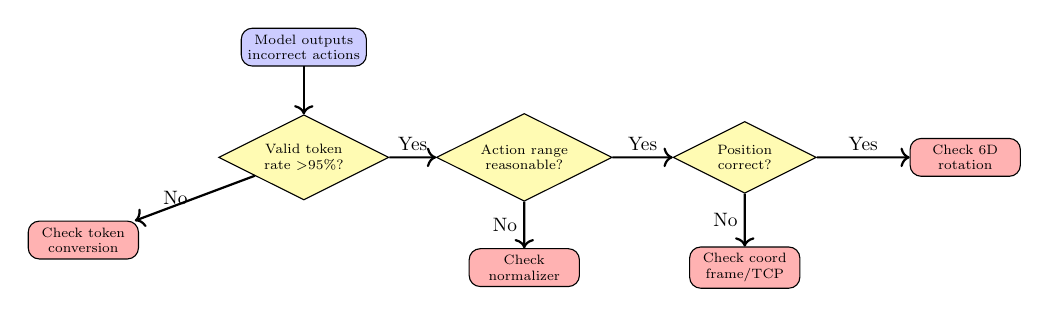
\begin{tikzpicture}[
        box/.style={rectangle, draw, rounded corners, minimum width=2cm, minimum height=0.6cm, align=center, font=\scriptsize},
        decision/.style={diamond, draw, aspect=2, minimum width=2cm, align=center, font=\scriptsize},
        arrow/.style={->, thick},
        scale=0.7, transform shape
    ]
        \node[box, fill=blue!20] (start) at (0,5) {Model outputs\\incorrect actions};

        \node[decision, fill=yellow!30] (valid) at (0,3) {Valid token\\rate $>$95\%?};

        \node[box, fill=red!30] (token_fix) at (-4,1.5) {Check token\\conversion};
        \node[decision, fill=yellow!30] (range) at (4,3) {Action range\\reasonable?};

        \node[box, fill=red!30] (norm_fix) at (4,1) {Check\\normalizer};
        \node[decision, fill=yellow!30] (orient) at (8,3) {Position\\correct?};

        \node[box, fill=red!30] (coord_fix) at (8,1) {Check coord\\frame/TCP};
        \node[box, fill=red!30] (rot_fix) at (12,3) {Check 6D\\rotation};

        \draw[arrow] (start) -- (valid);
        \draw[arrow] (valid) -- node[left] {No} (token_fix);
        \draw[arrow] (valid) -- node[above] {Yes} (range);
        \draw[arrow] (range) -- node[left] {No} (norm_fix);
        \draw[arrow] (range) -- node[above] {Yes} (orient);
        \draw[arrow] (orient) -- node[left] {No} (coord_fix);
        \draw[arrow] (orient) -- node[above] {Yes} (rot_fix);
    \end{tikzpicture}
    \end{center}
\end{frame}

%------------------------------------------------------------------------------
\begin{frame}{Testing Procedure}
    \textbf{Step-by-step verification:}

    \vspace(0.3cm)
    \begin{enumerate}
        \item \textbf{Sanity Check: Identity Action}
              \begin{itemize}
                  \item Feed action = current state
                  \item Model should output near-zero deltas
              \end{itemize}

        \item \textbf{Single Dimension Test}
              \begin{itemize}
                  \item Move only X position
                  \item Verify only X changes in action
              \end{itemize}

        \item \textbf{Known Trajectory}
              \begin{itemize}
                  \item Execute recorded human demo
                  \item Compare model output to ground truth
              \end{itemize}

        \item \textbf{Full Task Execution}
              \begin{itemize}
                  \item Run complete manipulation task
                  \item Evaluate success rate
              \end{itemize}
    \end{enumerate}
\end{frame}

%------------------------------------------------------------------------------
\begin{frame}{Creating Custom Normalizer}
    \textbf{For ManiSkill data:}

    \vspace(0.3cm)
    \begin{lstlisting}[language=Python, basicstyle=\ttfamily\small]
from models.normalizer import LinearNormalizer

# Collect action statistics from dataset
all_actions = []
for episode in dataset:
    all_actions.append(episode['actions'])
all_actions = np.concatenate(all_actions, axis=0)

# Create normalizer
normalizer = LinearNormalizer()
normalizer.fit({'action': all_actions}, mode='limits')

# Save
normalizer.save("maniskill_normalizer.pt")

# Or create manually
scale = 1.0 / (action_max - action_min)
offset = -action_min * scale
    \end{lstlisting}
\end{frame}

%------------------------------------------------------------------------------
\begin{frame}{Performance Benchmarks}
    \begin{table}
        \centering
        \renewcommand{\arraystretch}{1.3}
        \begin{tabular}{lccc}
            \toprule
            \textbf{Model} & \textbf{GPU} & \textbf{Latency} & \textbf{Real-time?} \\
            \midrule
            RDT2-VQ & RTX 4090 & $\sim$400ms & No \\
            RDT2-VQ (vLLM) & RTX 4090 & $\sim$237ms & Marginal \\
            RDT2-FM & RTX 4090 & $\sim$125ms & Yes \\
            RDT2-UltraFast & RTX 4090 & $\sim$100ms & Yes \\
            \bottomrule
        \end{tabular}
    \end{table}

    \vspace(0.3cm)
    \textbf{Real-time requirement:}
    \begin{itemize}
        \item Action chunk: 0.8s (24 frames @ 30Hz)
        \item Need inference $<$ 0.8s for continuous control
        \item Buffer time needed for safety margin
    \end{itemize}
\end{frame}

%------------------------------------------------------------------------------
\begin{frame}{Summary: Critical Points}
    \begin{columns}[T]
        \begin{column}{0.5\textwidth}
            \textbf{Must Verify:}
            \begin{itemize}
                \item Image: $384 \times 768$, RGB
                \item Tokens: $[0, 1023]$ range
                \item Normalizer: correct file
                \item Rotation: 6D format
                \item Gripper: rescaled
            \end{itemize}
        \end{column}
        \begin{column}{0.5\textwidth}
            \textbf{Common Pitfalls:}
            \begin{itemize}
                \item BGR vs RGB
                \item Wrong normalizer
                \item Token conversion
                \item Quaternion vs 6D
                \item Coordinate frame
            \end{itemize}
        \end{column}
    \end{columns}

    \vspace(0.5cm)
    \begin{alertblock}{Golden Rule}
        When in doubt, \textbf{print shapes and ranges} at every step. Most bugs are dimension or scale mismatches.
    \end{alertblock}
\end{frame}

%------------------------------------------------------------------------------
\begin{frame}{Resources}
    \textbf{Official Links:}

    \vspace(0.3cm)
    \begin{itemize}
        \item \textbf{GitHub:} \url{https://github.com/thu-ml/RDT2}
        \item \textbf{Project Page:} \url{https://rdt-robotics.github.io/rdt2/}
        \item \textbf{HuggingFace:}
              \begin{itemize}
                  \item RDT2-VQ: \code{robotics-diffusion-transformer/RDT2-VQ}
                  \item RDT2-FM: \code{robotics-diffusion-transformer/RDT2-FM}
                  \item Tokenizer: \code{robotics-diffusion-transformer/RVQActionTokenizer}
              \end{itemize}
    \end{itemize}

    \vspace(0.3cm)
    \textbf{Key Documentation:}
    \begin{itemize}
        \item \code{README.md} - Setup and usage
        \item \code{DEPLOYMENT\_TIPS.md} - Real robot tips
        \item \code{configs/} - Configuration examples
    \end{itemize}
\end{frame}



% Final slide
\begin{frame}{}
    \centering
    \vspace{2cm}
    {\Huge\bfseries Thank You}

    \vspace{1.5cm}
    {\Large Questions?}

    \vspace{1.5cm}
    \begin{tabular}{ll}
        GitHub: & \url{https://github.com/thu-ml/RDT2} \\
        Project: & \url{https://rdt-robotics.github.io/rdt2/} \\
    \end{tabular}
\end{frame}

\end{document}
